%% Harbor Methodology Bench --- whitepaper
%% Build:  tectonic -X compile main.tex   (or: make)
\documentclass[11pt,a4paper]{article}

\usepackage[T1]{fontenc}
\usepackage[utf8]{inputenc}
\usepackage{newtxtext,newtxmath}
\usepackage[a4paper,margin=2.4cm,bottom=2.8cm]{geometry}
\usepackage{graphicx}
\usepackage{booktabs}
\usepackage{multirow}
\usepackage{longtable}
\usepackage{array}
\usepackage{xcolor}
\usepackage{amsmath}
\usepackage[labelfont=bf,font=small,justification=raggedright,singlelinecheck=false]{caption}
\usepackage{enumitem}
\usepackage{microtype}
\usepackage{fancyhdr}
\usepackage{titlesec}
\usepackage[round]{natbib}
\usepackage[hidelinks]{hyperref}

\definecolor{accent}{HTML}{2A78D6}
\definecolor{warn}{HTML}{EB6834}
\definecolor{good}{HTML}{1BAF7A}
\definecolor{rule}{HTML}{B9B8AD}
\definecolor{shade}{HTML}{F5F5F2}

\hypersetup{colorlinks=true,linkcolor=accent,citecolor=accent,urlcolor=accent}
\setlist[itemize]{leftmargin=1.3em,itemsep=0.15em,topsep=0.3em}
\setlist[enumerate]{leftmargin=1.6em,itemsep=0.15em,topsep=0.3em}
\renewcommand{\arraystretch}{1.12}
\setlength{\tabcolsep}{5pt}
\titleformat{\section}{\normalfont\Large\bfseries\color{black}}{\thesection}{0.7em}{}
\titleformat{\subsection}{\normalfont\large\bfseries}{\thesubsection}{0.6em}{}
\titleformat{\subsubsection}{\normalfont\normalsize\bfseries}{\thesubsubsection}{0.6em}{}

\pagestyle{fancy}
\fancyhf{}
\fancyhead[L]{\small\color{black!55}Harbor Methodology Bench --- CodeZen vs SDD on Terminal-Bench 2.0}
\fancyhead[R]{\small\color{black!55}\thepage}
\renewcommand{\headrulewidth}{0.4pt}
\setlength{\emergencystretch}{2.5em}
\sloppy

% a boxed callout for the claims the paper wants to be quoted on
\newsavebox{\findingbox}
\newenvironment{finding}[1]
  {\par\medskip\noindent\begin{lrbox}{\findingbox}%
   \begin{minipage}{\dimexpr\linewidth-2\fboxsep-4pt}%
   \vspace{3pt}\textbf{\color{accent}#1}\par\smallskip\small}
  {\vspace{4pt}\end{minipage}\end{lrbox}%
   \noindent\textcolor{accent}{\vrule width 2pt height \dimexpr\ht\findingbox\relax depth \dimexpr\dp\findingbox\relax}%
   \colorbox{shade}{\usebox{\findingbox}}\par\medskip}

% \code and \task must be breakable: many are long paths and task slugs
\newcommand{\bt}{\discretionary{}{}{}}
\newcommand{\code}[1]{\texttt{\small #1}}
\newcommand{\task}[1]{\texttt{\footnotesize #1}}

\begin{document}

\begin{titlepage}
\centering
\vspace*{2.2cm}
{\color{accent}\rule{\linewidth}{1.2pt}}\\[0.7cm]
{\LARGE\bfseries Does a Repository's Agent Configuration\\[0.25cm]
Make a Coding Agent Better, Worse,\\[0.25cm] or Merely More Expensive?\par}
\vspace{0.5cm}
{\large A controlled measurement of two software methodologies\\
on Terminal-Bench 2.0, over 156 trials and two opposite task populations\par}
\vspace{0.4cm}
{\color{accent}\rule{\linewidth}{1.2pt}}\\[1.2cm]

{\large Christoph Mitschka\par}
\vspace{0.15cm}
{\small \href{mailto:christoph.mitschka@korza.ai}{christoph.mitschka@korza.ai}\par}
\vspace{0.4cm}
{\small with an independent critical review contributed by \textbf{Antigravity} (Google DeepMind),\\
whose analysis is integrated throughout and adjudicated in Section~\ref{sec:divergence}\par}
\vspace{1.4cm}

\begin{minipage}{0.86\linewidth}\small
\textbf{Abstract.} Coding agents are increasingly deployed inside repositories that carry a
declared engineering process: a \code{CLAUDE.md}, an \code{AGENTS.md}, a skills directory, a
kit of templates. Whether that configuration improves the agent's work, or only its token
bill, is usually argued rather than measured. We measure it. Two published agent toolkits
--- \textbf{CodeZen}, a delegation-and-review toolkit, and \textbf{SDD}, a seven-step
specification chain --- were frozen at a Git SHA, injected as a Docker layer into
Terminal-Bench 2.0 task containers, and proven present from inside each container before any
trial ran. Against a proven-clean \textbf{baseline} we ran 156 trials over 26 tasks and two
task populations selected on opposite criteria: one where the bare agent fails
(\emph{suite}, 16 tasks) and one where it already succeeds (\emph{ceiling}, 10 tasks). Total
model spend was \$201.37 over 30.1 hours of agent wall-clock on \code{claude-sonnet-5}.
\textbf{No outcome effect was detectable for either toolkit} on either population, and
neither population could have shown one reliably: every McNemar test is non-significant, and
on \emph{suite} the coarse and fine outcome metrics do not even rank the conditions the same
way. That is an underpowered and inconsistent null, not a demonstrated absence.
\textbf{Both changed the cost, one of them substantially}: CodeZen costs $1.71\times$
baseline on work that completes (dearer on 10 of 10 tasks, $p = 0.002$) and $3.11\times$ on
work that does not ($p = 0.009$), for $0.96$--$1.00\times$ the partial credit. The binding
constraint is not money but the clock: CodeZen consumed $1.90\times$ baseline's share of the
declared time budget and was killed on 25\,\% of its trials, and 7 of the 23 kills across
both runs discarded a workspace the verifier would have scored 1.0. One solved task was
turned unsolved by process. Availability was total and adherence was not: 71\,\% of toolkit
trials invoked no toolkit skill at all. The much-quoted conclusion that repeated independent
sampling dominates methodology at equal spend does not survive a heterogeneity-aware
estimator, and we bound it rather than assert it. The largest methodological finding is
about the experiment: both task screens overshot, because a one-trial inclusion rule cannot
distinguish a task the agent \emph{always} fails from one it \emph{sometimes} fails, and only
the second discriminates.
\end{minipage}

\vfill
{\small\color{black!55}Runs executed 2026-08-31 to 2026-09-01 \quad$\cdot$\quad
document compiled \today \quad$\cdot$\quad
task suite pinned at \code{2fd12b88}}
\end{titlepage}

\tableofcontents
\clearpage

\section{Introduction}
\label{sec:intro}

A modern coding agent rarely works on a bare task. It works inside a repository, and that
repository hands it a configuration: instruction files it loads silently, skills it can
invoke, standards documents, kit templates, slash commands. The industry has produced a
growing number of such configurations, marketed as methodologies --- do test-driven
development, review your own diff, write a specification before you write code --- and the
question of whether any of them helps is normally settled by assertion.

This paper reports a measurement instead. The question it was built to answer is narrow
enough to be answerable:

\begin{finding}{The question}
Does working inside a repository configured with a coding methodology make a coding agent
better, worse, or merely more expensive --- and does the agent actually follow the
methodology when it is available?
\end{finding}

\noindent Both halves are load-bearing. A configuration that is present but unused is a
finding about the toolkit, not about methodology in general, so availability and adherence
are instrumented separately and reported separately.

\subsection{What is new here relative to the source analyses}

This document consolidates two per-run analyses, one cross-run synthesis, and an independent
critical review of all three contributed by Antigravity (Google DeepMind). Every finding in
those documents is carried forward. Nothing has been dropped. Where the two readings
disagree --- on numbers, on emphasis, or on what a result licenses --- Section
\ref{sec:divergence} states the disagreement, recomputes the quantity from the exported
trial tables, and says which reading survives.

Five contributions are new to this paper:

\begin{enumerate}
\item \textbf{Full recomputation.} Every number quoted here was recomputed from the exported
      per-trial tables by \code{whitepaper/scripts/verify\_numbers.py}, independently of both
      source discussions. This surfaced six arithmetic slips in the independent review and two in
      the primary reading; all are in Section~\ref{sec:divergence}, and one of them changes a
      story rather than only a number.
\item \textbf{An independence check on the retry argument.} The claim that repeated
      independent sampling dominates methodology at equal spend rests on
      $P(\text{success}) = 1 - (1-p)^k$, which assumes every attempt on every task is a draw
      from one common Bernoulli rate. The two-attempt design lets us test that assumption.
      It leans the wrong way in five of six run $\times$ condition cells
      (Section~\ref{sec:bestofn}).
\item \textbf{A bounded verdict on Best-of-$N$.} With three estimators --- homogeneous,
      beta-binomial, and per-task plug-in --- the equal-spend comparison spans 37\,\% to
      83\,\% against CodeZen's 50\,\% on the \emph{suite} population. The conclusion is
      therefore \emph{estimator-dependent}, and we report it as a range rather than a verdict.
\item \textbf{Conventions and clustering made explicit.} All three censoring conventions are
      reported side by side rather than two of them (Tables~\ref{tab:outcome-suite}
      and~\ref{tab:outcome-ceiling}); every interval on a test-level rate is a task-clustered
      bootstrap rather than a binomial interval on test rows, which widens them by 24 to 30
      points and puts the effective sample size at 16--20 in \emph{suite}; and the one trial
      of 156 with no per-test record is documented, along with what it does to the
      partial-credit ordering it happens to decide (Section~\ref{sec:metrics}).
\item \textbf{Twenty figures and seven diagrams}, several of which visualise results the
      source documents state only in prose: the flatness of the cost multiplier against a
      $288\times$ range of task length, the dissolution of the length effect as the outcome
      metric sharpens, and what a one-trial screen actually selects for.
\end{enumerate}

\subsection{Summary of findings}

\begin{finding}{Settled by the pair of runs}
\begin{enumerate}[nosep]
\item CodeZen costs $1.71\times$ baseline on work that completes and $3.11\times$ on work
      that does not, for $0.96$--$1.00\times$ the partial credit. Significant on two
      independent populations.
\item SDD costs $\approx 1.1\times$ and is behaviourally near-invisible, but satisfies
      $0.82$--$0.83\times$ of each verifier's tests --- consistently across both runs,
      without reaching significance in either.
\item Methodology can regress a solved task, and can make a solved task less reliable.
\item 71\,\% of toolkit trials invoked no toolkit skill at all.
\item Human-expert difficulty does not predict agent difficulty ($\rho = -0.078$, $p = 0.70$).
\item The screens' single-trial inclusion rule is unreliable in both directions, and both
      screens overshot.
\end{enumerate}
\end{finding}

\begin{finding}{Not established by either run}
\begin{enumerate}[nosep]
\item Any claim about which configuration produces better outcomes. 18 of 26 tasks are
      concordant and the effective sample size per pairwise test is 1--5.
\item That SDD's partial-credit shortfall is real rather than noise ($p = 0.125$ at $n = 10$).
\item Any causal reading of ``trials that invoked a skill mostly failed''; this design cannot
      separate selection from effect.
\item That Best-of-$N$ retries beat methodology at equal spend. The sign of that comparison
      changes with the estimator (Section~\ref{sec:bestofn}).
\item Anything about the regime methodologies are actually written for: multi-session work
      with ambiguous requirements and a human in the loop.
\end{enumerate}
\end{finding}

\section{Related work: process, agents, and bounded compute}
\label{sec:related}

The argument this paper joins runs in six steps. Each is established elsewhere; only the last
is ours.

\paragraph{A. Software engineering uses process to improve quality, and the evidence for that
is real.} Test-driven development is associated with better internal and external quality in
systematic review \citep{bissi2016tdd} and in industry experiment \citep{tosun2017industry},
and code review is a load-bearing quality practice in professional development. Nothing in
this paper disputes any of that, and any reading of it as ``testing and review do not work''
is a misreading.

\paragraph{B. Process also has measurable productivity and latency costs.} The same TDD
literature reports mixed-to-negative productivity effects alongside the quality gains
\citep{bissi2016tdd,tosun2017industry}, and it has proven hard even to attribute the quality
benefit to writing tests first rather than to working in short verified cycles
\citep{fucci2017dissection}. On the review side, speed --- not thoroughness alone --- is what
determines when work reaches users \citep{kudrjavets2024review}. Process is a trade, and the
trade has always had two sides.

\paragraph{C. Autonomous agents operate in a different resource regime.} Agentic software
engineering research argues explicitly that language-model agents are a new category of end
user, with interfaces, needs and failure modes distinct from a human developer's
\citep{yang2024sweagent}; interactive agent evaluation finds weak long-horizon reasoning and
instruction following to be dominant failure modes \citep{liu2024agentbench}; and a
deliberately simple pipeline can match elaborate agent scaffolding on repository tasks
\citep{xia2024agentless}. The regime, not just the speed, is different.

\paragraph{D. In that regime, additional machinery consumes a scarce inference-time resource.}
Tool-augmented reasoning does not automatically beat a plain chain of thought, and its
overhead decomposes into prompt formatting, protocol cost and genuine execution benefit
\citep{zhang2026tooltax}. More generally, the productive use of an extra unit of test-time
compute depends sharply on instance difficulty \citep{snell2024scaling}, and agent evaluations
have begun to treat resource efficiency as a dependent variable rather than an externality
\citep{liu2026costbench}. Human process research measures cost in calendar time; here the
currency is the same bounded budget that must also produce the artefact.

\paragraph{E. Whether specification helps depends on what the task actually requires.}
Specification processes address ambiguity and quality defects in natural-language requirements
\citep{femmer2017smells} --- but the effort of hunting ambiguity is not always repaid, and its
value is contingent on context \citep{ribeiro2020ambiguity}. Process research reaches the same
conclusion from the other direction: a standardised process should be \emph{tailored} to its
project rather than applied unchanged \citep{xu2007tailoring}.

\paragraph{F. Therefore a benchmark of fully specified, single-session tasks may systematically
under-test the value of a specification process --- and a benchmark with a hard wall-clock may
systematically over-expose the cost of any process at all.} That is this paper's contribution,
and it is why the outcome null of Section~\ref{sec:outcome} is reported as uninformative rather
than as a refutation, while the cost and clock results of Sections~\ref{sec:cost} and
\ref{sec:clock} are reported as the findings. Two further strands support the design
criticism directly: single-run agent performance estimates carry substantial between-run
variance \citep{bjarnason2026randomness}, which is what breaks the one-trial task screen
(Section~\ref{sec:floor}); and audits of widely used coding benchmarks find a material share
of tasks affected by overly strict tests or underspecified prompts \citep{openai2026signal},
which is what makes task-set construction a first-order concern rather than a detail. Where
human expert time is used as the difficulty axis, we follow the convention that defines an
agent's task-completion horizon in those terms \citep{kwa2025horizons}.

\clearpage
\section{Experimental design}
\label{sec:design}

\subsection{Terminal-Bench 2.0: the benchmark underneath everything}

Terminal-Bench 2.0 \citep{merrill2026terminalbench} is an agentic coding benchmark from the
Laude Institute, Stanford and Snorkel AI. Each task is a containerised terminal environment plus a natural-language
instruction; an agent is dropped into the container with a shell and a wall-clock budget, and
a verifier runs afterwards to decide whether the work was done. The pool holds 89 tasks
across 16 categories at easy, medium and hard difficulty. Three properties of that design
determine how this experiment must be read.

\begin{itemize}
\item \textbf{The reward is a verifier, not a judge.} A task passes when its own test suite
      passes: each task ships a unique environment, a human-written solution and tests written
      to verify it \citep{merrill2026terminalbench}. No model grades style or process, so a
      methodology can only score by changing the artefact on disk. This is a strength: it
      removes the most common way for a process evaluation to flatter itself.
\item \textbf{Tasks are self-contained and fully specified.} The instruction states what
      done means, and the success criterion is machine-checkable. Specification processes are
      motivated largely by the opposite situation: natural-language requirements carry
      ambiguity and quality defects that must be surfaced before behaviour can be agreed
      \citep{femmer2017smells}, and the effort of surfacing them is itself of
      context-dependent value \citep{ribeiro2020ambiguity}. A fully specified, automatically
      graded task removes much of that class of difficulty by construction --- which makes
      this the regime in which a specification process has \emph{least} to add, and is a
      threat to validity we return to in Section~\ref{sec:threats}. Note also that the
      benchmark's difficulty metadata is human expert time, the same quantity used to define
      agent task-completion horizons \citep{kwa2025horizons}; Section~\ref{sec:length} shows
      it predicts almost nothing about this agent.
\item \textbf{Every task declares a wall-clock budget}, and Harbor enforces it. That single
      fact turns out to be the dominant mechanism in the entire dataset
      (Section~\ref{sec:clock}).
\end{itemize}

Harbor builds each task's image, runs the agent inside it, runs the verifier, and writes the
reward, token counts, cost and a full agent trajectory to disk. The task suite is pinned at
commit \code{2fd12b88}; no task was modified.

\subsection{What \code{harbor-methodology-bench} adds}

The naive version of this experiment silently measures nothing. Harbor transfers only
\code{instruction.md}, \code{tests/} and \code{solution/} into a container, so a
\code{CLAUDE.md} placed next to \code{task.toml} never reaches the agent. The framework
therefore injects the methodology as a \textbf{Docker layer} on top of the task's own base
image, and then proves from \emph{inside} each container that the condition is what was
declared.

\begin{center}\small
\begin{tabular}{@{}ll@{}}
\toprule
Question & Answered by \\
\midrule
Was the methodology \textbf{available} to the agent? & \code{hmb preflight} --- an assertion made inside the container \\
Did the agent \textbf{use} it? & \code{hmb analysis} --- adherence read from the agent's own trajectory \\
\bottomrule
\end{tabular}
\end{center}

The generated Dockerfile is byte-identical across every condition of a task, and the
\code{baseline} container's working directory is proven byte-identical to the untouched base
image, so no build-path difference can be mistaken for a methodology effect. All 48 task
variants in the \emph{suite} run and all 30 in the \emph{ceiling} run passed preflight before
a single trial started. Figure~\ref{fig:pipeline} shows the pipeline.

\begin{figure}[htbp]
\centering
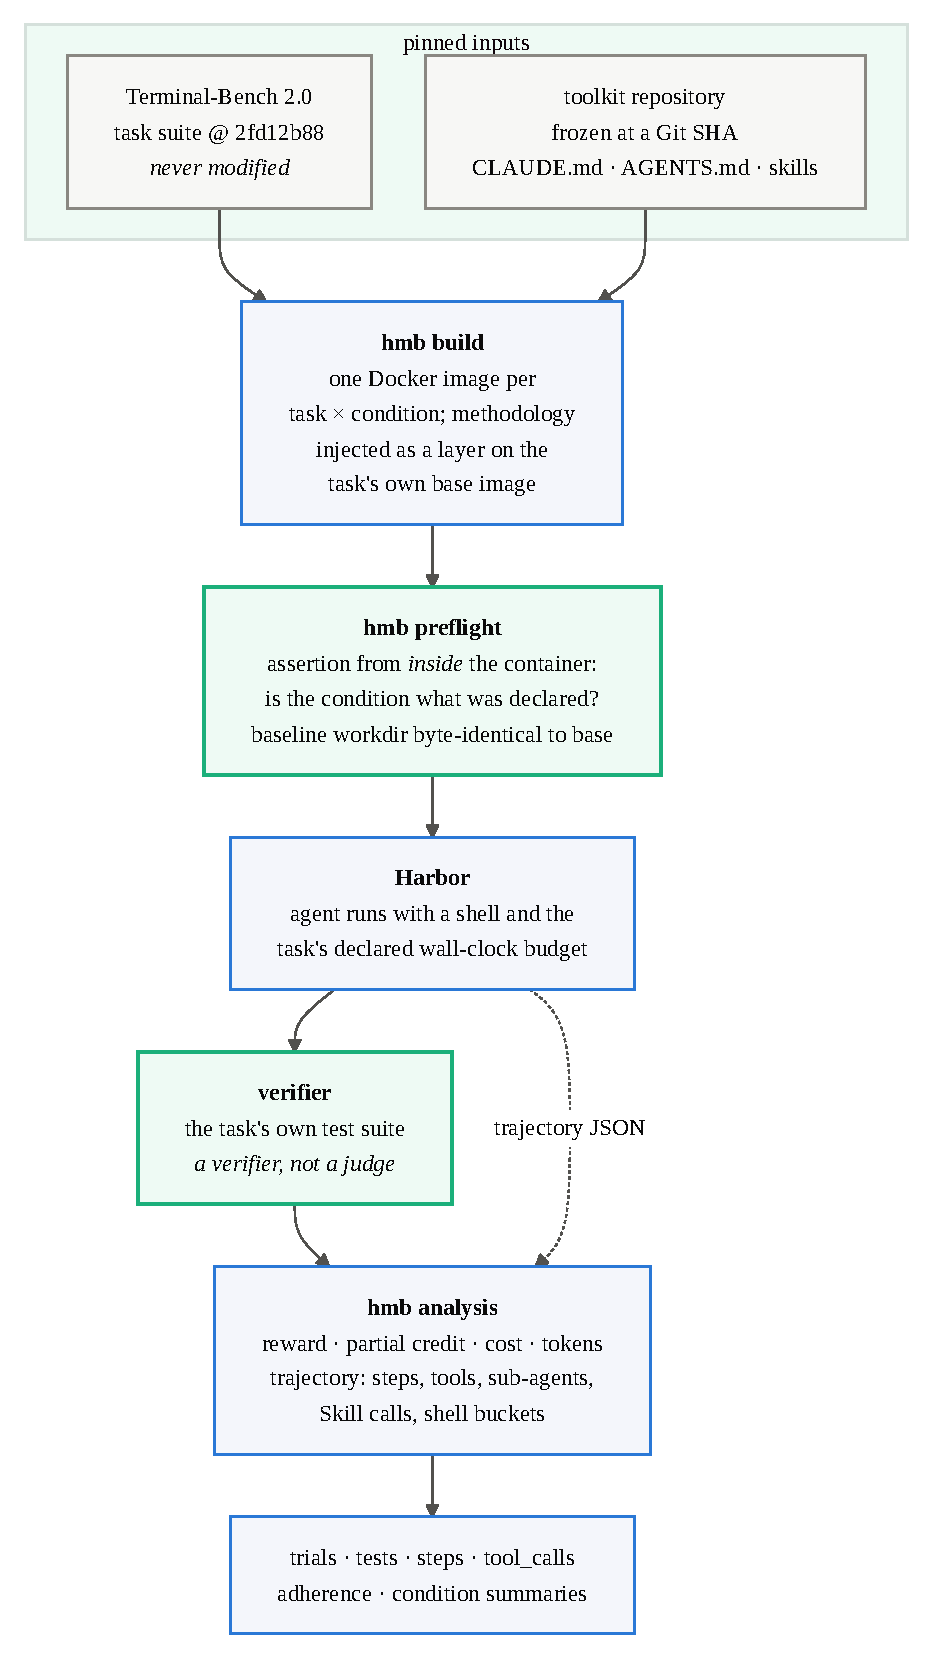
\includegraphics[width=0.70\linewidth]{diagrams/d02-measurement-pipeline.pdf}
\caption{The measurement pipeline. The two checks in green are what separate this design
from an experiment that cannot tell a present configuration from an absent one:
\code{preflight} asserts availability from inside the container, and the task's own verifier
--- not a model --- decides the reward.}
\label{fig:pipeline}
\end{figure}

\subsection{The three conditions}

\begin{center}\small
\begin{tabular}{@{}p{2.6cm}p{12.4cm}@{}}
\toprule
Condition & What the agent's working directory contains \\
\midrule
\code{baseline} & the benchmark task and nothing else --- the pure agent, proven clean \\
\code{sdd} & the SDD toolkit as shipped: \code{CLAUDE.md}, \code{AGENTS.md}, \code{.sdd-kit/},
and 7 installed skills (\code{sdd-specify}, \code{sdd-clarify}, \code{sdd-plan},
\code{sdd-tasks}, \code{sdd-analyze}, \code{sdd-implement}, \code{sdd-verify}) \\
\code{codezen-viable} & the CodeZen plugin reprojected as a repository, restricted to the 4
skills that can run inside a benchmark container: \code{noc-tdd}, \code{noc-fix},
\code{code-review}, \code{security-review} \\
\bottomrule
\end{tabular}
\end{center}

\code{codezen-viable} is a curated subset \emph{by necessity}: CodeZen's other seven skills
need a Docker daemon, a human, a running system under test, or the Notion MCP server, none of
which exist in a benchmark container. That is a stated confound, not an oversight, and it
means every CodeZen result below is a result about a four-skill subset.

The agent is Claude Code on \code{claude-sonnet-5} in all conditions. Sub-agents spawned by
CodeZen's skills run the \emph{same} model, which matters for interpreting delegation
(Section~\ref{sec:behaviour}).

\subsection{Where these runs sit in a longer sequence}

\begin{figure}[htbp]
\centering
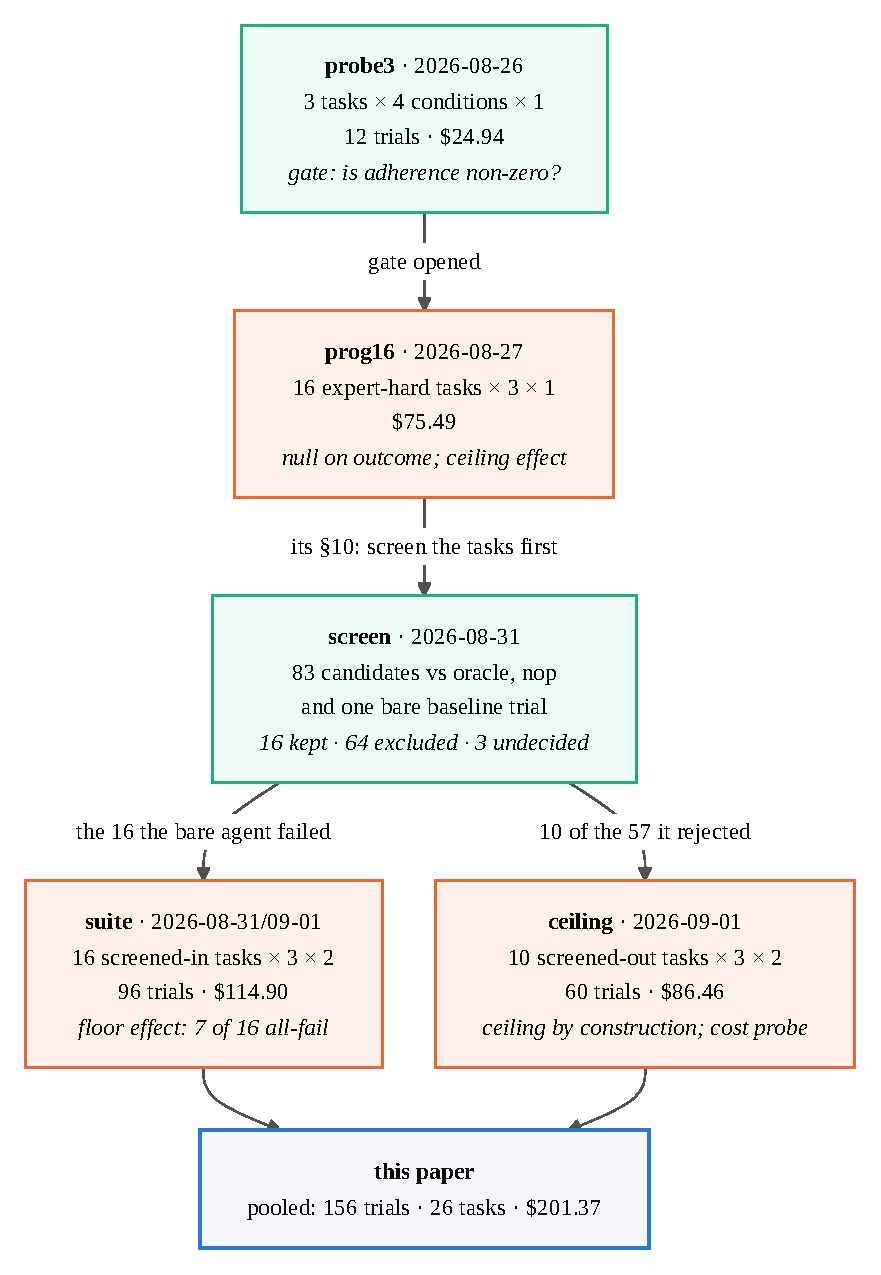
\includegraphics[width=0.80\linewidth]{diagrams/d01-experiment-sequence.pdf}
\caption{The run sequence. Each run's design was chosen to repair the previous run's defect,
and the repair overshot every time: selecting for human-expert difficulty produced a ceiling,
screening for ``the bare agent fails'' produced a floor, and the rejected set is a ceiling by
construction.}
\label{fig:sequence}
\end{figure}

The two runs analysed here are the last two in a five-run sequence. \emph{probe3} (12 trials,
\$24.94) was a gate on whether the full measurement was worth paying for; its predicted null
--- zero adherence --- did not happen, so the gate opened. \emph{prog16} (16 tasks selected
for human-expert difficulty, \$75.49) returned a null on outcome, a measured cost, and a
ceiling effect that made the null uninformative; its recommendation was to screen candidate
tasks first. \emph{screen} executed that recommendation over 83 candidates, keeping 16 and
excluding 64. The two runs reported here are the screen's two sides.

\subsection{The two task populations}

\begin{table}[htbp]
\centering
\caption{The two populations, selected on opposite criteria. The line that matters is the
last but one: in both runs, most of the money bought tasks on which every condition did the
same thing.}
\label{tab:populations}
\small

\begin{tabular}{@{}lrr@{}}
\toprule
 & \textbf{suite} & \textbf{ceiling} \\
\midrule
Inclusion rule & bare agent must fail & bare agent already passes \\
Tasks $\times$ conditions $\times$ attempts & $16\times3\times2$ & $10\times3\times2$ \\
Trials & 96 & 60 \\
Model spend & \$114.90 & \$86.46 \\
Agent wall-clock & 18.3\,h & 11.8\,h \\
Baseline pass-at-2 & 6/16 = 37.5\% & 9/10 = 90.0\% \\
Concordant tasks (pass-at-2) & 10/16 & 8/10 \\
\quad all three pass / all three fail & 3 / 7 & 8 / 0 \\
Spend on concordant tasks & \$74.47 (65\%) & \$54.46 (63\%) \\
Effective $n$ per pairwise test & 4--5 & 1--2 \\
Design defect & floor effect & ceiling, by construction \\
Intended endpoint & outcome & cost and regression \\
\bottomrule
\end{tabular}

\end{table}

The \emph{suite} population is a derivation, not a selection: every task in it survived
\code{hmb screen}, meaning the oracle agent scored 1.0, the \code{nop} agent scored 0.0, and
one bare baseline trial failed. The \emph{ceiling} population is ten of the 57 tasks the same
screen \emph{rejected} for being at ceiling, ranked by expert estimate $\div$ agent budget
and the top ten under $32\times$ taken --- on the reasoning that a high ratio means the
ceiling that excluded the task is shallowest. Full task tables, with categories, expert
estimates, budgets and per-condition outcomes, are in Appendix~\ref{app:tasks}.

One correlation to note before any task-level result is read: \task{path-tracing-reverse} in
the \emph{ceiling} set is a sibling of \task{path-tracing} in the \emph{suite} set. The two
are not independent samples.

\subsection{Metrics, and the two conventions that change conclusions}
\label{sec:metrics}

\paragraph{Outcome, at three resolutions.} The binary \textbf{reward} is the task's own
verdict. \textbf{Partial credit} is the mean fraction of a task's verifier tests that passed:
one continuous observation per trial in place of one bit, which is a real gain in resolution
at unchanged $n$. \textbf{Test-level pass rate} pools individual verifier tests across a
condition: 357 graded test outcomes in \emph{suite}, 162 in \emph{ceiling}.

Those pooled counts are \emph{not} 357 independent observations, and this paper does not treat
them as such. Tests within a task share a workspace, a verifier and a failure mode, and the
clusters are severely unbalanced --- \task{adaptive-rejection-sampler} and \task{sam-cell-seg}
contribute 18 rows each while \task{configure-git-webserver} contributes 2, so two of 16 tasks
supply 30\,\% of a condition's rows. Every interval quoted on a test-level rate in this paper
is therefore a bootstrap that resamples whole \emph{tasks}, not a binomial interval on test
rows. The resulting design effects are 5.7--7.4 in \emph{suite} and 1.6--3.6 in
\emph{ceiling}, putting the effective sample size at 16--20 and 15--34 respectively: finer
resolution per trial, no extra statistical power. When a coarse metric and a fine metric
disagree, the fine one is the better-resolved, and Section~\ref{sec:outcome} contains exactly
that disagreement.

\paragraph{One trial has no per-test record, and it matters.} Of the 156 trials, exactly one
--- \task{torch-tensor-parallelism} under baseline in \emph{suite} --- carries no per-test
outcomes at all. It was not censored: the agent finished inside 34\,\% of budget, and the
verifier then ran for 436.8\,s, nearly twice the 204--255\,s it took on the other five trials
of that task, and returned reward 0 with no test rows. Every other trial in both runs has a
complete per-test breakdown. Baseline's \emph{suite} partial credit of 0.533 is therefore a
mean over 31 trials, not 32; scoring that trial 0 --- which is what it was, a graded failure
--- gives 0.517 instead. Section~\ref{sec:outcome} reports the consequence rather than picking
one of the two, because the choice is load-bearing for exactly one claim and the claim is a
close one.

\paragraph{Convention 1: what a timeout means.} Harbor kills the agent at the task's declared
budget and grades whatever is on disk. Three readings are defensible, and they are all
reported here:

\begin{enumerate}[label=\textbf{\arabic*.}]
\item \textbf{censored} --- the trial leaves both numerator and denominator, because the agent
      was stopped, not beaten. Denominator: graded trials. This is the primary convention
      below.
\item \textbf{timeout = failure} --- every trial is in the denominator and a kill counts
      against the condition that provoked it, whatever was on disk. Numerator: graded passes
      only.
\item \textbf{graded at the kill} --- every trial is in the denominator and a censored trial
      keeps the reward the verifier actually assigned to the workspace that was killed. Seven
      of the 23 censored trials scored 1.0, so this reading recovers observations the other
      two throw away.
\end{enumerate}

\noindent All three are reported as separate columns of
Tables~\ref{tab:outcome-suite} and~\ref{tab:outcome-ceiling}, numbered as here. Readings 2
and 3 share a denominator and differ only over whether a censored pass counts, so the
difference between those two columns is exactly the censored-but-passing trials. Reading 3 is
the per-attempt quantity the equal-spend retry argument of Section~\ref{sec:bestofn} needs,
because it is the probability that one attempt ends with a passing workspace; reading 2 is the
punitive bound. A fourth arrangement --- crediting censored passes while still discarding
censored failures --- is arithmetically available and is not used anywhere here, because it
keeps the winners and censors the losers.

The choice is not cosmetic. In the \emph{ceiling} run it moves CodeZen by 12.9 points from
reading 1 to reading 3 and by 27.9 points from reading 1 to reading 2, taking it from first
place to second and to third respectively (Section~\ref{sec:outcome-ceiling}). It must be fixed in
writing before a run, not after seeing the numbers.

\paragraph{Convention 2: what ``the task passed'' means at two attempts.} With
\code{--attempts 2} there are two defensible definitions, and they disagree about the run's
most interesting claim:

\begin{itemize}
\item \textbf{pass-at-2} --- passed at least one attempt. The standard multi-attempt reading.
\item \textbf{pass-both} --- passed both attempts. This is a \emph{reliability} measure, and
      it is what \code{data/outcome\_matrix.csv} actually writes, under a filename that
      implies the other definition. That is a reporting trap worth naming.
\end{itemize}

Under pass-at-2, SDD regressed no task in the \emph{ceiling} run. Under pass-both, it
regressed three. Both are reported throughout, because for an operator reliability is the
relevant property and choosing the flattering definition is not available.

\paragraph{Budget consumption} is agent wall-clock divided by the task's declared budget from
\code{task.toml}. Nine trials ran concurrently on one host, so wall-clock --- and therefore
budget consumption --- carries host contention. Cost and token metrics do not. Because
contention is symmetric across conditions within a task, the paired comparisons remain valid;
the absolute budget percentages are inflated.

\subsection{Statistical methods}

Every task ran in every condition, so the correct tests are paired. Binary outcomes use the
exact McNemar test (equivalently, a two-sided binomial test on the discordant pairs).
Continuous per-trial quantities use the Wilcoxon signed-rank test on per-task means.
Proportions carry Wilson 95\,\% intervals. Length relationships use two-sided Spearman rank
correlations, and the \code{long-horizon} axis split uses Mann--Whitney $U$.

Power is stated wherever a null is reported, because at these sample sizes a $p$ above 0.05
means \emph{not resolved}, not \emph{absent}. From the Fisher $z$ transformation, 80\,\% power
at $\alpha = 0.05$ two-sided requires $|\rho| \ge 0.53$ at $n = 26$, $\ge 0.65$ at $n = 16$,
and $\ge 0.79$ at $n = 10$. Note also that $p = 0.002$ is the \emph{minimum attainable}
$p$-value for a two-sided Wilcoxon test at $n = 10$: when the \emph{ceiling} run reports it,
the correct reading is ``the effect is present on every single task'', not ``the effect is
large''.

\clearpage
\section{Results I: outcome}
\label{sec:outcome}

\subsection{The \emph{suite} run: a null, and metrics that disagree}

\begin{table}[htbp]
\centering
\caption{\emph{suite} outcome by condition. 16 tasks $\times$ 3 conditions $\times$ 2
attempts, so 32 trials per condition. The three numbered blocks are the three censoring
conventions of Section~\ref{sec:metrics}: \textbf{1} drops censored trials from numerator and
denominator, \textbf{2} puts all 32 trials in the denominator with graded passes only in the
numerator, \textbf{3} puts all 32 in the denominator and lets a censored trial keep the reward
the verifier assigned it. Partial credit is over every trial that has a per-test record: 32
for CodeZen and SDD, 31 for baseline, whose \task{torch-tensor-parallelism} failure produced
none. Test rate pools verifier tests and is clustered within tasks; see the clustered
intervals in the text.}
\label{tab:outcome-suite}
\small

\begin{tabular}{@{}lrrrrcrrrrr@{}}
\toprule
 & & & & \multicolumn{2}{c}{\textbf{1.} censored} & \multicolumn{1}{c}{\textbf{2.} t/o} &
 \multicolumn{1}{c}{\textbf{3.} graded} & & & \\
\cmidrule(lr){5-6}\cmidrule(lr){7-7}\cmidrule(lr){8-8}
 & \multicolumn{1}{c}{cens.} & \multicolumn{1}{c}{graded} &
 \multicolumn{1}{c}{passed} & \multicolumn{1}{c}{rate} & \multicolumn{1}{c}{95\,\% Wilson} &
 \multicolumn{1}{c}{$=$ fail} & \multicolumn{1}{c}{at kill} &
 \multicolumn{1}{c}{part.\ credit} &
 \multicolumn{1}{c}{test rate} & \multicolumn{1}{c}{spend} \\
\midrule
baseline & 4 & 28 & 7 & 25.0\% & [12.7, 43.4] & 21.9\% & 25.0\% & 0.533 & 59.8\% & \$21.87 \\
CodeZen & 7 & 25 & 9 & 36.0\% & [20.2, 55.5] & 28.1\% & 34.4\% & 0.516 & 60.0\% & \$68.13 \\
SDD & 3 & 29 & 7 & 24.1\% & [12.2, 42.1] & 21.9\% & 21.9\% & 0.448 & 52.5\% & \$24.89 \\
\bottomrule
\end{tabular}

\end{table}

\begin{figure}[htbp]
\centering
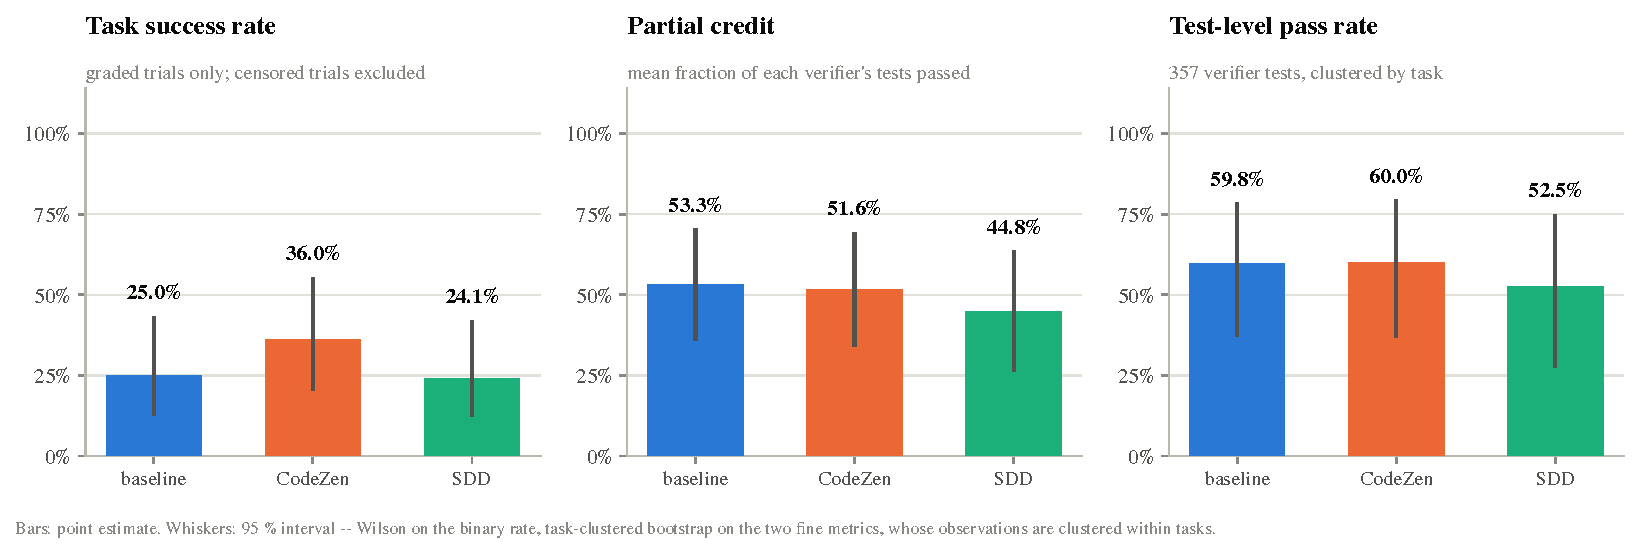
\includegraphics[width=\linewidth]{figures/suite-01-outcome.pdf}
\caption{\emph{suite}: the coarse metric and the fine metrics disagree. Success rate ranks
CodeZen first by 11 points; partial credit ranks baseline first by 0.017, which one
unrecorded trial reduces to 0.0007; test-level pass rate separates SDD from the other two and
puts baseline and CodeZen within 0.2 points of each other. Whiskers on the two fine panels
are task-clustered bootstrap intervals, not binomial intervals on test rows.}
\label{fig:outcome-suite}
\end{figure}

\textbf{The metrics disagree, and that is the finding.} Success rate ranks CodeZen first by
11 points, on a difference of two trials. Partial credit --- a continuous score per trial
rather than a bit, on the same trials --- ranks baseline first, with CodeZen 0.017 below and
SDD 0.085 below. That 0.017 does not survive the one trial with no per-test record: baseline's
0.533 is a mean over 31 trials, and scoring its \task{torch-tensor-parallelism} failure 0, as
Section~\ref{sec:metrics} sets out, gives 0.517 against CodeZen's 0.516 --- a gap of 0.0007,
which is a tie in everything but the fourth decimal. Test-level pass rate reproduces neither
ordering either: CodeZen is 0.2 points \emph{above} baseline there (60.0\,\% against
59.8\,\%), a coin flip, and the only visible structure in that panel is SDD's 7-point
shortfall.

If a methodology effect existed and the binary reward were merely too coarse to see it,
partial credit is where it would appear first. What the fine metrics show is not the absence
of an effect --- the intervals below are wide enough to contain a moderate real effect in
either direction --- but \textbf{no detectable effect that the fine metric and the coarse
metric agree about}. Success rate moves one way on two trials, partial credit moves the other
way, and the test-level rate moves neither. The defensible summary is ``underpowered and
inconsistent'', not ``null confirmed''. Nor is the partial-credit ordering itself robust: it
rests on one unrecorded trial, and CodeZen's paired partial-credit ratio moves from
$0.96\times$ ($p = 1.000$, lower on 3 of 16 tasks) to $1.00\times$ ($p = 0.837$) between the
two readings of that trial. SDD's shortfall is the only fine-metric signal that survives both
readings, at $0.83\times$ and $0.87\times$.

The Wilson intervals contain each other completely: at $n = 25$--$29$, the interval on 36\,\%
runs from 20\,\% to 56\,\%, and one task moves the point estimate by about 4 points. Under
pass-at-2 the exact McNemar test gives $p = 0.625$ for baseline against CodeZen (4 discordant
tasks, CodeZen winning 3) and $p = 1.000$ against SDD (5 discordant).

\textbf{The fine metric is finer, not larger.} The 357 test-level outcomes sit inside 16
tasks, and unevenly: \task{adaptive-rejection-sampler} and \task{sam-cell-seg} contribute 18
rows each, \task{configure-git-webserver} 2. Resampling whole tasks gives design effects of
5.7 (baseline), 6.2 (CodeZen) and 7.4 (SDD) and effective sample sizes of 20.4, 19.4 and 16.3
--- \emph{fewer} effective observations than the 25--29 graded trials the binary rate rests
on. The clustered 95\,\% intervals are [37.1, 78.6] for baseline, [36.8, 79.5] for CodeZen and
[27.3, 75.0] for SDD --- 42, 43 and 48 points wide against binomial intervals on the same
counts that are 17, 17 and 18 points wide. So partial credit
earns its extra resolution honestly, by replacing one bit with a continuous score on the same
trials; the pooled test count does not buy power, and no power claim is made for it here.

\textbf{The censoring convention moves the magnitudes and compresses the ordering.} Counting a
kill as a failure (reading 2) gives baseline 21.9\,\%, CodeZen 28.1\,\% and SDD 21.9\,\%;
grading the killed workspace (reading 3) gives 25.0\,\%, 34.4\,\% and 21.9\,\%. CodeZen is
nominally first on the binary metric under all three readings and behind on the finer ones
under all three, but its lead shrinks from 11 points to 6 under the strictest reading, and
baseline and SDD become a tie rather than an ordering.

\begin{finding}{Three of these kills were solved tasks, which is a harness defect and not a
robustness check}
\task{path-tracing} under baseline, and \task{adaptive-rejection-sampler} and
\task{torch-tensor-parallelism} under CodeZen, were killed by the clock with a \emph{passing}
verifier already on disk (reward 1.0). Readings 2 and 3 do not bracket an uncertainty about
those trials: they record the same three solved tasks as failures and as passes, on identical
evidence. Seven of the 23 kills across both runs are of this kind. The correct response is not
a choice between those two columns but the recognition that the evidence already exists:
Harbor graded each of those workspaces, and reading 3 is the column that uses what it found.
An analysis whose primary endpoint is reading 3 loses no observation to the clock at all.
Section~\ref{sec:clock} treats it as the measurement defect it is.
\end{finding}

\noindent \textbf{The one ordering that is not in dispute is the price.} CodeZen spent
\$68.13 against baseline's \$21.87 and SDD's \$24.89, or $3.11\times$ baseline, to buy a
two-trial success-rate lead that no test separates from noise together with partial credit and
a test-level rate that are level with or below baseline's. Per graded pass that is \$7.57
against \$3.12 and \$3.56. Read as a hypothesis test this table is a null; read as a
procurement decision it is not neutral, and the cost ratio is the larger takeaway.
Section~\ref{sec:costeff} measures it properly, including the \$23.13 per marginal success
CodeZen's two extra passes actually cost.

\subsection{Could the \emph{suite} design have measured anything? The screen overcorrected}
\label{sec:floor}

\begin{figure}[htbp]
\centering
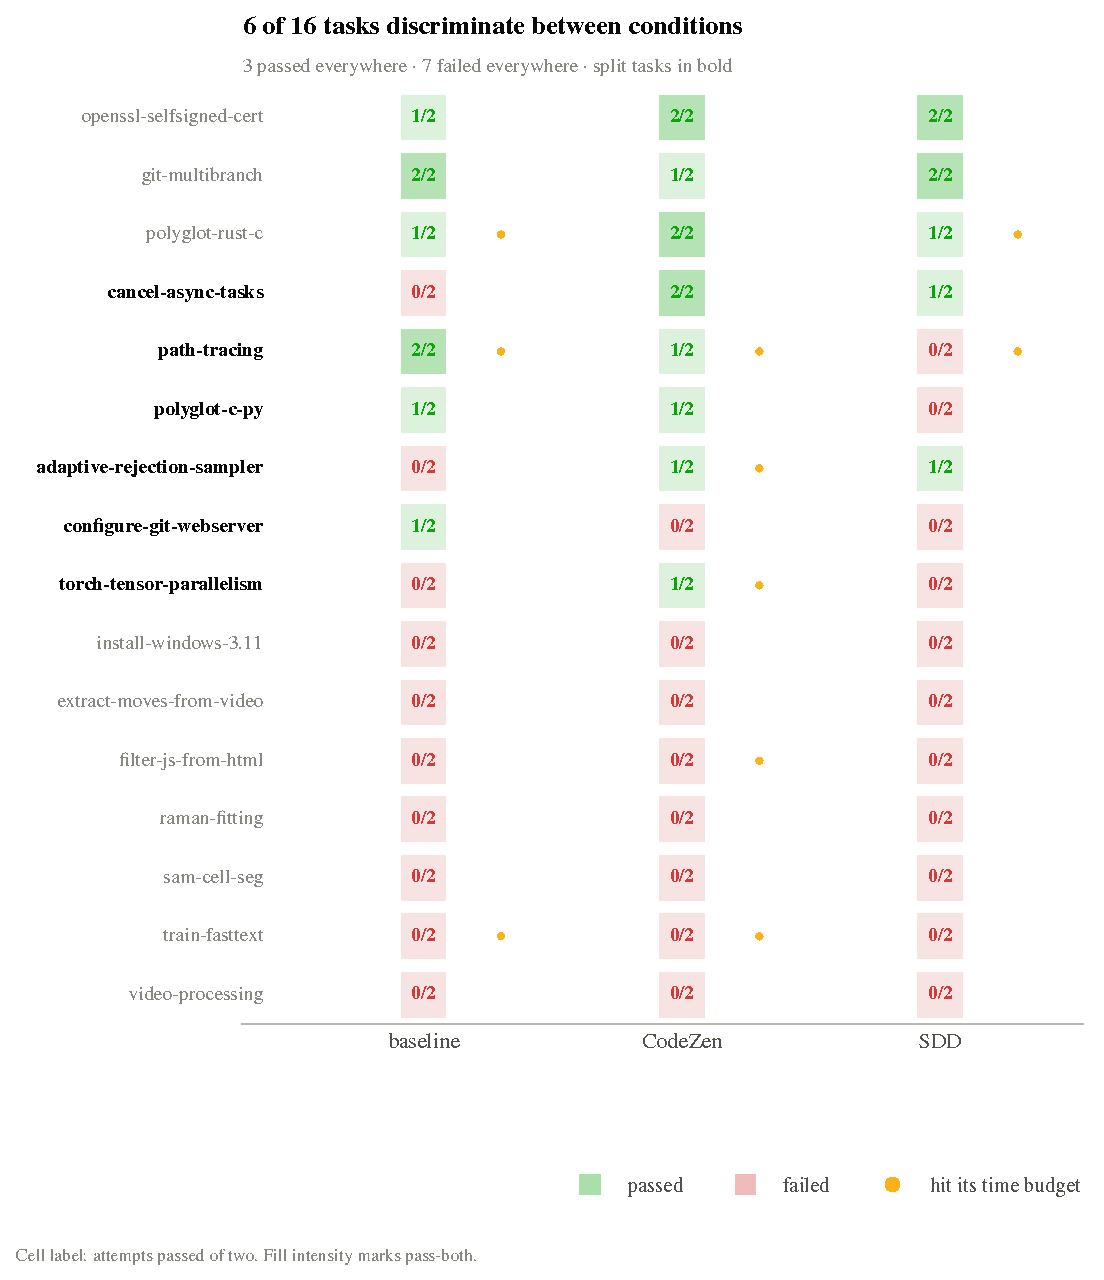
\includegraphics[width=0.94\linewidth]{figures/suite-02-outcome-matrix.pdf}
\caption{\emph{suite} task $\times$ condition outcomes. A paired comparison learns nothing
from a row where every condition does the same thing, and 10 of these 16 rows are of that
kind --- seven of them failed by everything.}
\label{fig:matrix-suite}
\end{figure}

Ten of 16 tasks are concordant under pass-at-2: three passed by all three conditions
(\task{git-multibranch}, \task{openssl-selfsigned-cert}, \task{polyglot-rust-c}) and
\textbf{seven failed by all three} (\task{extract-moves-from-video},
\task{filter-js-from-html}, \task{install-windows-3.11}, \task{raman-fitting},
\task{sam-cell-seg}, \task{train-fasttext}, \task{video-processing}). Those ten tasks
consumed \textbf{\$74.47 of the \$114.90 spent}, or 65\,\%, and carried no information. The
effective sample size per pairwise comparison is 4 to 5, not 16. Under pass-both the picture
is worse: \emph{zero} tasks pass in all three conditions, 11 fail in all three, and baseline
passes both attempts on 2 of 16 tasks.

\begin{finding}{The floor effect is the mirror image of the ceiling effect it was built to fix}
\begin{center}\small
\begin{tabular}{@{}llrrr@{}}
\toprule
Run & Task set & Baseline pass-at-2 & Concordant & Effective $n$ \\
\midrule
\emph{prog16} & selected for human-expert difficulty & 13/16 = 81\,\% & 11/16 (ceiling) & 2--5 \\
\emph{suite} & screened: bare agent must fail & \textbf{6/16 = 37.5\,\%} & 10/16 (floor) & 4--5 \\
\emph{ceiling} & screened: bare agent must pass & 9/10 = 90\,\% & 8/10 (ceiling) & 1--2 \\
\bottomrule
\end{tabular}
\end{center}
The screen ran exactly as specified, excluded 64 of 83 candidates, and produced a set whose
effective sample size is no better than the run it was designed to repair.
\end{finding}

\noindent The defect is in the rule, and it is specific. The screen includes a task when the
bare agent fails it on \textbf{one} trial. Recent evidence makes that a quantified problem
rather than a suspicion: over roughly 60{,}000 agent trajectories on SWE-Bench-Verified,
single-run performance estimates vary substantially between runs, including at temperature
zero \citep{bjarnason2026randomness}. A one-trial screen therefore samples run-to-run noise
as much as it samples task difficulty. One trial cannot distinguish \emph{always fails} ---
a floor task, concordant, carrying no information --- from \emph{sometimes fails}, the only
kind of task that discriminates. Figure~\ref{fig:screen} makes the arithmetic explicit: the
one-trial rule is monotone in the wrong quantity. A hopeless task passes the screen with
certainty; an ideally discriminating task is discarded half the time.

\begin{figure}[htbp]
\centering
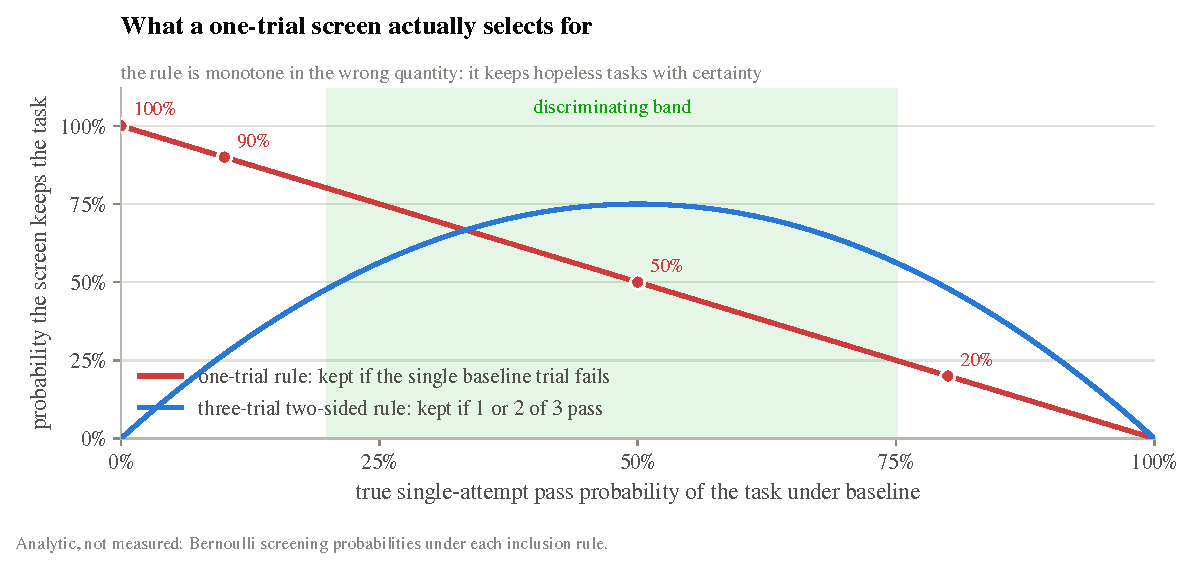
\includegraphics[width=0.84\linewidth]{figures/x13-screen-selection.pdf}
\caption{What a one-trial exclusion rule selects for, analytically. The red curve is the
probability that a task with true single-attempt pass probability $p$ is kept by the rule
``keep it if one baseline trial fails''. It peaks exactly where the task is useless. The blue
curve is a two-sided rule on three trials, which peaks inside the discriminating band.}
\label{fig:screen}
\end{figure}

\begin{figure}[htbp]
\centering
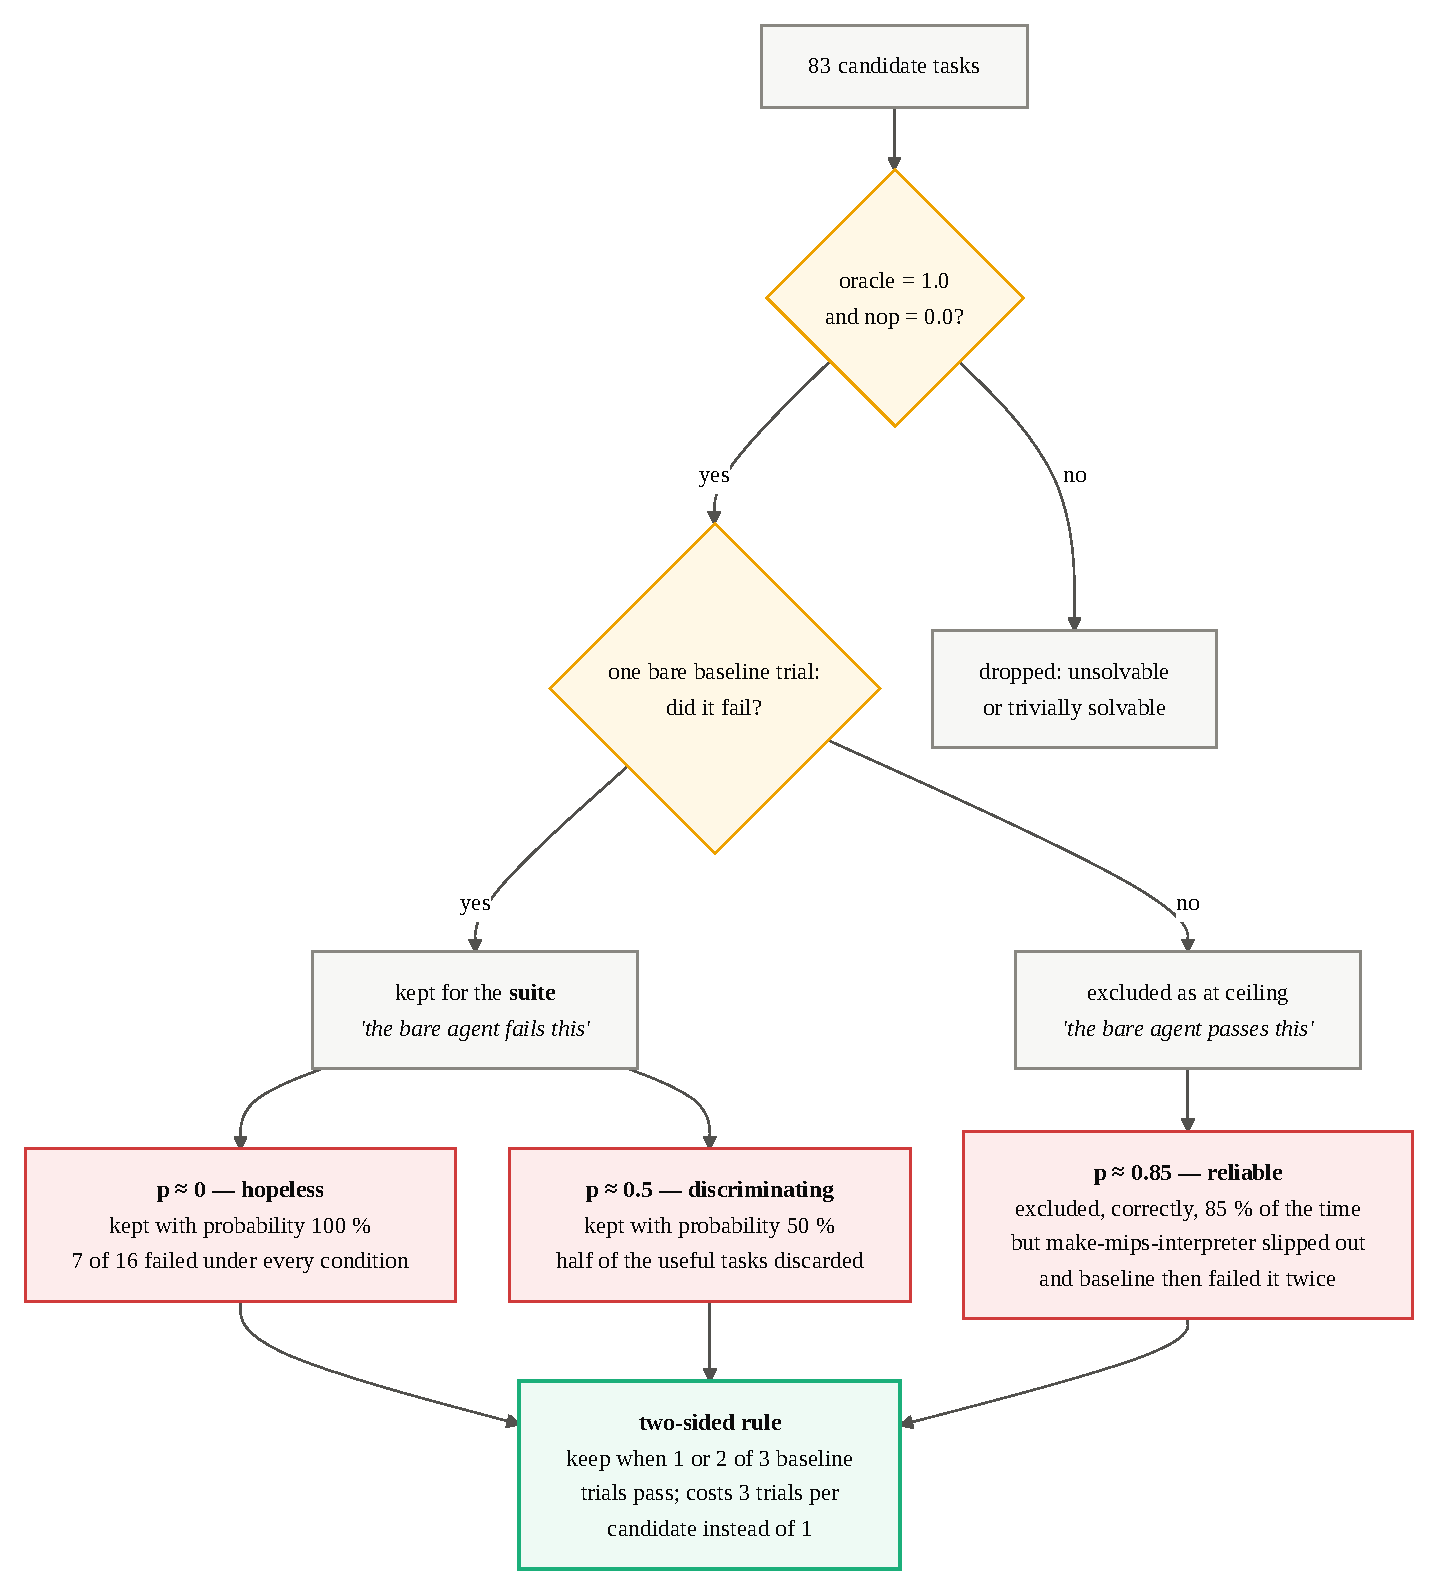
\includegraphics[width=0.80\linewidth]{diagrams/d06-screen-defect.pdf}
\caption{The same defect as a decision path, with the three misclassification modes the data
actually exhibits. \task{make-mips-interpreter} was excluded as ``the bare agent already
passes it'' on one trial, and baseline then failed both of its attempts in the \emph{ceiling}
run.}
\label{fig:screen-defect}
\end{figure}

\subsection{The \emph{ceiling} run: at ceiling by design, and the censoring flip}
\label{sec:outcome-ceiling}

\begin{table}[htbp]
\centering
\caption{\emph{ceiling} outcome by condition. 10 tasks $\times$ 3 conditions $\times$ 2
attempts, so 20 trials per condition; numbered blocks as in
Table~\ref{tab:outcome-suite}. Success rate is \emph{not} an endpoint of this run --- the
population was selected to be at ceiling --- and is stated so that the next paragraph can show
why it must not be read as a result.}
\label{tab:outcome-ceiling}
\small

\begin{tabular}{@{}lrrrrcrrrrr@{}}
\toprule
 & & & & \multicolumn{2}{c}{\textbf{1.} censored} & \multicolumn{1}{c}{\textbf{2.} t/o} &
 \multicolumn{1}{c}{\textbf{3.} graded} & & & \\
\cmidrule(lr){5-6}\cmidrule(lr){7-7}\cmidrule(lr){8-8}
 & \multicolumn{1}{c}{cens.} & \multicolumn{1}{c}{graded} &
 \multicolumn{1}{c}{passed} & \multicolumn{1}{c}{rate} & \multicolumn{1}{c}{95\,\% Wilson} &
 \multicolumn{1}{c}{$=$ fail} & \multicolumn{1}{c}{at kill} &
 \multicolumn{1}{c}{part.\ credit} &
 \multicolumn{1}{c}{test rate} & \multicolumn{1}{c}{spend} \\
\midrule
baseline & 1 & 19 & 17 & 89.5\% & [68.6, 97.1] & 85.0\% & 85.0\% & 0.917 & 90.7\% & \$22.72 \\
CodeZen & 6 & 14 & 13 & 92.9\% & [68.5, 98.7] & 65.0\% & 80.0\% & 0.900 & 92.6\% & \$38.80 \\
SDD & 2 & 18 & 14 & 77.8\% & [54.8, 91.0] & 70.0\% & 75.0\% & 0.750 & 68.5\% & \$24.94 \\
\bottomrule
\end{tabular}

\end{table}

\begin{figure}[htbp]
\centering
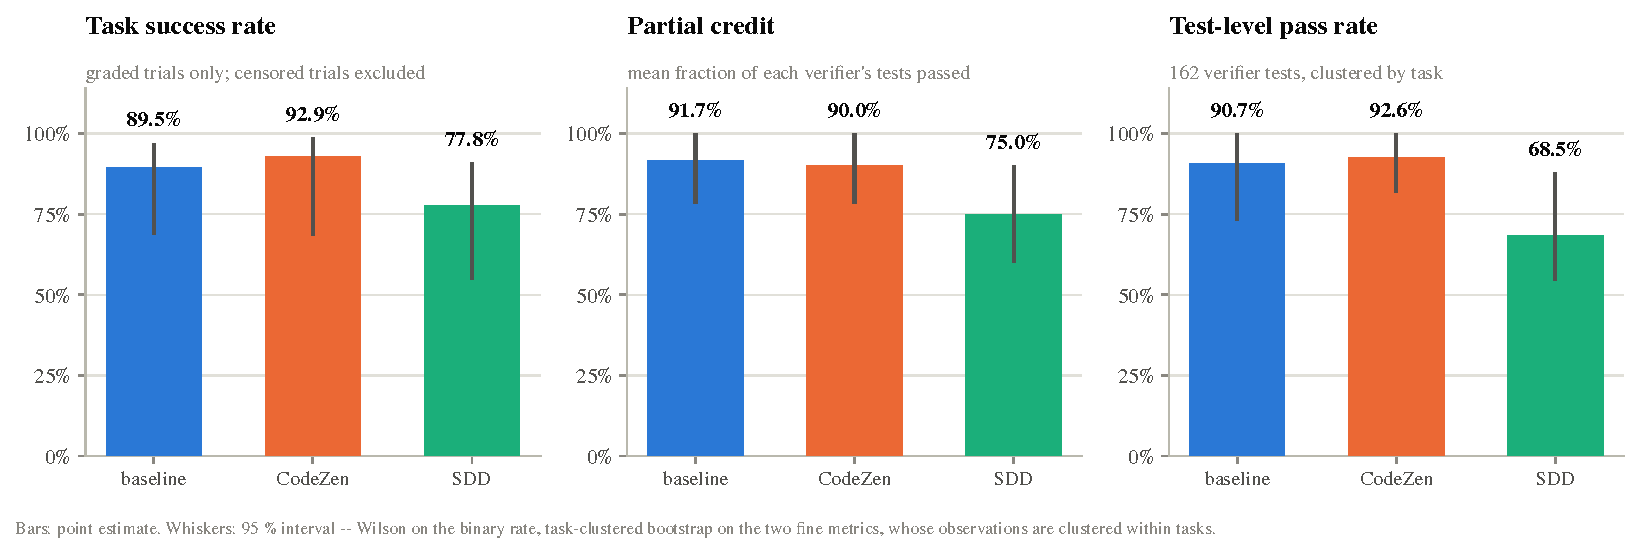
\includegraphics[width=\linewidth]{figures/ceiling-01-outcome.pdf}
\caption{\emph{ceiling}: the three Wilson intervals overlap almost completely on the binary
metric, and every pairwise McNemar test returns $p = 1.000$. The one panel worth taking
seriously is the third: SDD satisfies 22 points less of each verifier than baseline does. Its
whiskers are task-clustered bootstrap intervals and they still overlap --- the shortfall is
carried by the paired comparison, not by this figure.}
\label{fig:outcome-ceiling}
\end{figure}

The task set is at ceiling, as designed: baseline passes 89.5\,\% of graded trials. No
success-rate ordering here is a result. What the outcome section of this run \emph{does}
establish is that the censoring convention changes the answer:

\begin{finding}{The censoring convention flips the ranking}
\begin{center}\small
\begin{tabular}{@{}lrrr@{}}
\toprule
Condition & 1. censored & 2. timeout $=$ failure & 3. graded at kill \\
\midrule
\code{baseline} & 89.5\,\% & \textbf{85.0\,\% (1st)} & \textbf{85.0\,\% (1st)} \\
\code{codezen-viable} & \textbf{92.9\,\% (1st)} & 65.0\,\% (3rd) & 80.0\,\% (2nd) \\
\code{sdd} & 77.8\,\% & 70.0\,\% (2nd) & 75.0\,\% (3rd) \\
\bottomrule
\end{tabular}
\end{center}
CodeZen moves from first to \emph{third} and loses 27.9 points under the punitive reading,
because it is censored on 6 of 20 trials against baseline's 1. Four of the nine kills in this
run scored reward 1.0, three of them CodeZen's, so most of that 27.9-point swing is the
convention rather than the methodology --- the two all-trial readings disagree with each other
by 15 points on CodeZen and by 0 on baseline. The convention is doing more work here than any
measured effect does. Reading 3 is the one to prefer, because it is the only one that uses the
evidence Harbor already collected rather than discarding it or overruling it; it is not the
primary convention of this paper only because the two source analyses were written against
reading 1.
\end{finding}

\noindent \textbf{SDD's fine-grained metrics are the exception worth taking seriously.}
Partial credit 0.750 against baseline's 0.917, and test-level pass rate 68.5\,\% against
90.7\,\% --- a 22-point gap across 54 verifier tests per condition. Unlike the binary rates
this is not a two-trial artefact; it is a consistent shortfall in how much of each task's test
suite SDD satisfied. The strength of the claim comes from the pairing rather than from the
54 rows: clustered by task, the intervals are [54.4, 88.0] for SDD and [72.9, 100.0] for
baseline and they overlap, whereas the paired test on per-task means puts the shortfall at
ratio 0.818, $p = 0.125$ on 10 tasks --- not significant, lower on 4 of 10 tasks and higher on
1, and the largest and most consistent negative signal anywhere in either run.

\begin{figure}[htbp]
\centering
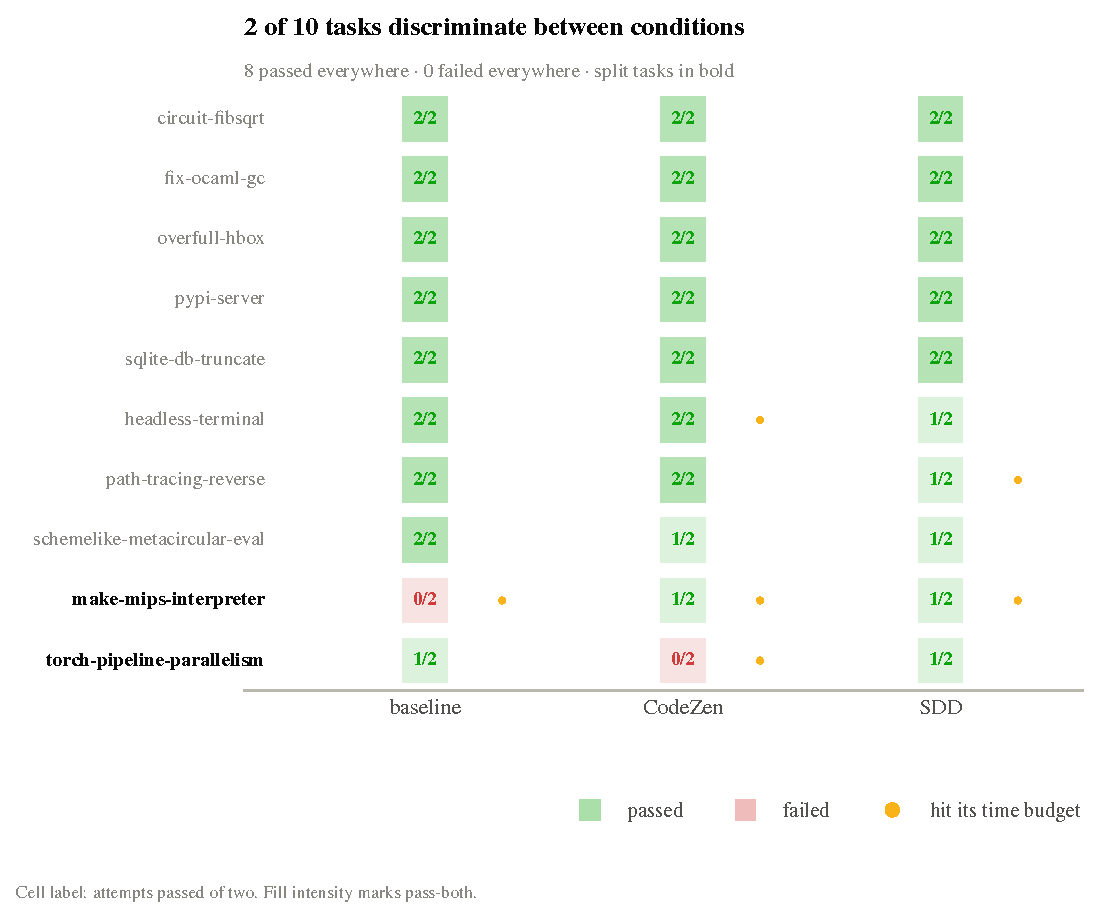
\includegraphics[width=0.80\linewidth]{figures/ceiling-02-outcome-matrix.pdf}
\caption{\emph{ceiling} task $\times$ condition outcomes. Concordance is this population's
defining property rather than a defect; what matters is which two tasks broke ranks, and both
are the two highest expert/budget ratios in the set.}
\label{fig:matrix-ceiling}
\end{figure}

\subsection{Regressions: where process made a solved task unsolved}
\label{sec:regressions}

In a ceiling experiment, any failure on a task the bare agent solves is prima facie evidence
of methodology-induced harm. Under \textbf{pass-at-2} there is exactly one such case, and it
is clean:

\begin{finding}{\task{torch-pipeline-parallelism}: a solved task made unsolved}
Baseline passes it on one of two attempts, using \textbf{29\,\% of its declared budget}
and 3 of 3 tests --- its other attempt failed at 2 of 3 inside 38\,\% of budget, so baseline is
itself only half reliable here and the mean budget consumption across its attempts is 34\,\%.
CodeZen invoked \code{code-review} on one attempt and \code{noc-tdd} + \code{code-review} on
the other, consumed \textbf{100\,\% of budget on both}, and failed both times at 2 of 3 tests
(partial credit 0.67). The task needs delicate synchronisation across pipeline stages; the
review sub-agents analysed code style and test architecture while the synchronisation bug went
unfixed. The mechanism is in the trajectory, not inferred --- but the honest version of the
claim is ``a task baseline solves half the time, that CodeZen never solved, at three times the
budget'', not ``a task baseline solves easily''.
\end{finding}

\noindent CodeZen also \emph{gained} \task{make-mips-interpreter} under pass-at-2, and SDD
lost nothing and gained the same task. Under \textbf{pass-both} the regression list grows:
CodeZen additionally loses \task{schemelike-metacircular-eval}; SDD loses
\task{headless-terminal}, \task{path-tracing-reverse} and \task{schemelike-metacircular-eval}.

The gap between the two SDD readings consists entirely of tasks SDD passed once and failed
once --- tasks it made \emph{less reliable} without making them impossible. In the
\emph{suite} run the same two readings give: CodeZen lost \task{configure-git-webserver} and
gained three; SDD lost \task{configure-git-webserver}, \task{path-tracing} and
\task{polyglot-c-py} and gained two.

\begin{finding}{On the selection rule, from the data}
\task{make-mips-interpreter} and \task{torch-pipeline-parallelism} are the two highest
expert/budget ratio tasks in the \emph{ceiling} set ($16\times$ each), and they are also the
two that broke ranks. The ranking rule did what it was meant to --- it found the shallowest
ceilings --- but it overshot at the top of the range: these two tasks are not reliably at
ceiling at all. Baseline failed \task{make-mips-interpreter} on \emph{both} attempts here,
having been recorded by the screen as a task ``the bare agent already passes''. That is
direct evidence, from the other side, of the same single-trial defect that produced the
\emph{suite} run's floor.
\end{finding}

\clearpage
\section{Results II: cost}
\label{sec:cost}

Cost is a continuous per-trial quantity rather than a rare binary event, so it is measurable
at $n = 10$--$16$ where the outcome is not. This is where both runs deliver.

Treating it as a primary endpoint rather than a footnote follows a broader shift: agent
evaluations have tended to emphasise task completion while under-weighting resource
efficiency \citep{liu2026costbench}, and the machinery an agent is given is not automatically
worth its price --- tool-augmented reasoning has been shown to carry a measurable
\emph{tool-use tax}, separable into prompt-formatting cost, protocol overhead and genuine
execution benefit \citep{zhang2026tooltax}. What follows is the repository-process analogue of
that accounting, and the difference should be stated rather than elided: that work measures
tool-call overhead inside a single agent, whereas the object here is repository-level process
scaffolding and the procedural skills a checkout makes available. Read alongside the finding
that the return on extra inference-time compute varies sharply with instance difficulty
\citep{snell2024scaling}, the question this section answers is not ``is process expensive''
but ``what does the price buy, and on which tasks''.

\subsection{Two multipliers, measuring different things}

\begin{figure}[htbp]
\centering
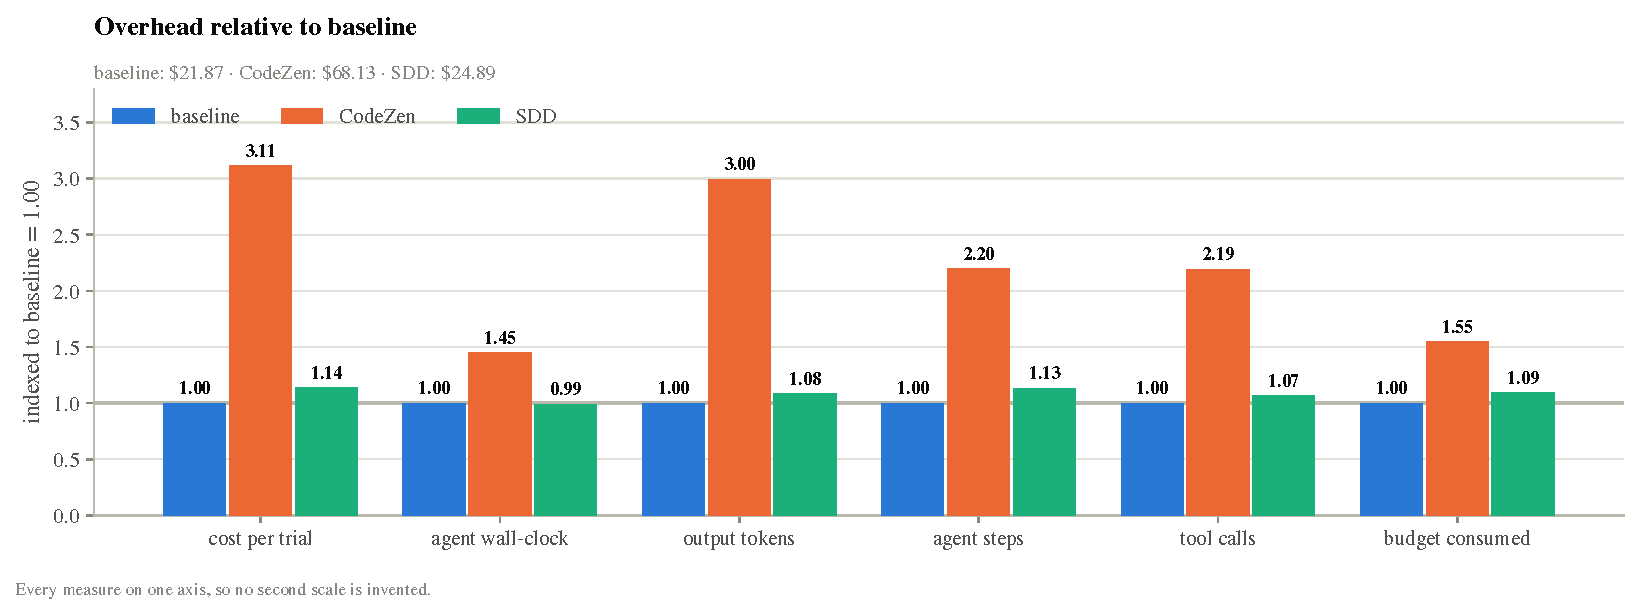
\includegraphics[width=\linewidth]{figures/suite-03-overhead.pdf}\\[0.5em]
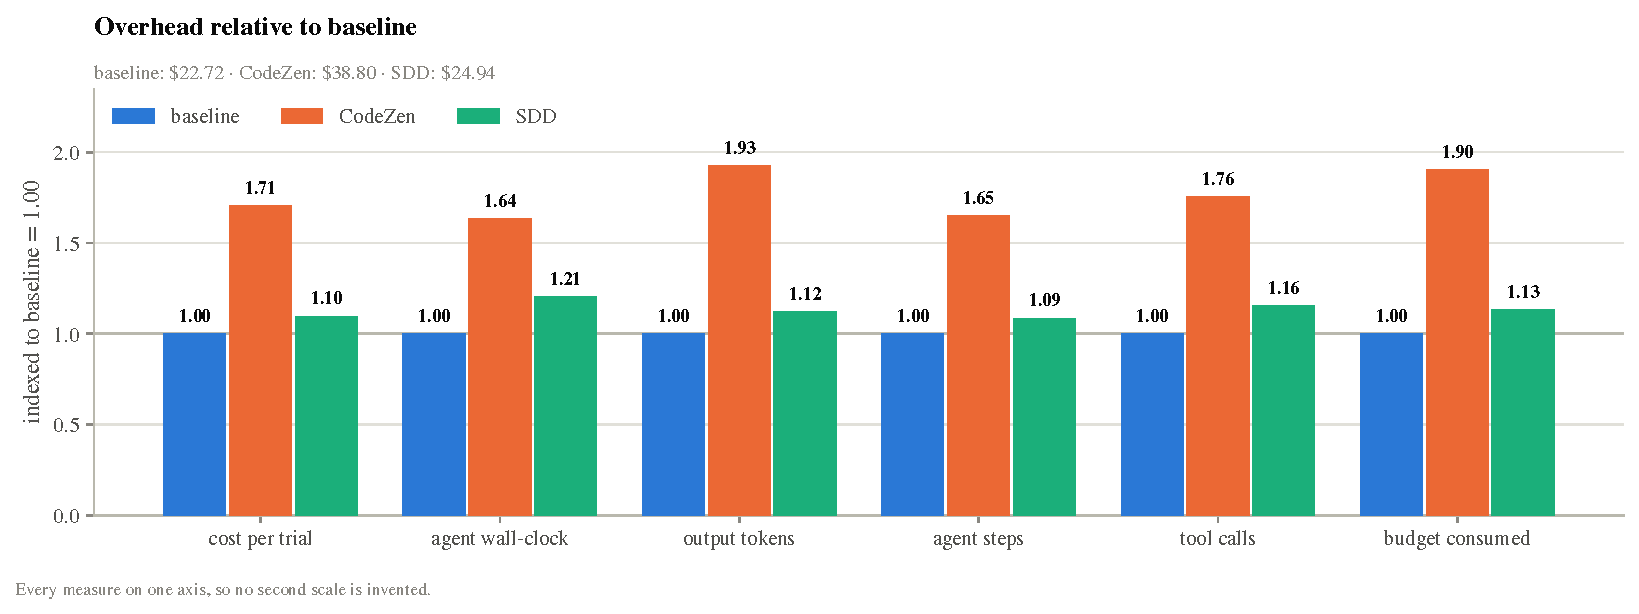
\includegraphics[width=\linewidth]{figures/ceiling-03-overhead.pdf}
\caption{Overhead indexed to baseline. Top: \emph{suite}, where work mostly aborts. Bottom:
\emph{ceiling}, where work mostly completes. Every measure is on one axis, so no second scale
is invented. SDD is within noise of baseline on both populations; CodeZen is not.}
\label{fig:overhead}
\end{figure}

\begin{table}[htbp]
\centering
\caption{Paired tests, \emph{suite} ($n = 16$ tasks). Wilcoxon signed-rank on per-task means;
``higher on'' counts tasks where the condition exceeded baseline. Bold marks $p < 0.05$.}
\label{tab:paired-suite}
\small

\begin{tabular}{@{}lrcrrcr@{}}
\toprule
 & \multicolumn{3}{c}{CodeZen vs baseline} & \multicolumn{3}{c}{SDD vs baseline} \\
\cmidrule(lr){2-4}\cmidrule(lr){5-7}
metric & ratio & higher on & \multicolumn{1}{c}{$p$} & ratio & higher on & \multicolumn{1}{c}{$p$} \\
\midrule
cost (\$) & 3.115 & 12/16 & \textbf{0.009} & 1.138 & 9/16 & 0.821 \\
budget consumed & 1.548 & 10/16 & 0.093 & 1.094 & 6/16 & 0.782 \\
agent wall-clock & 1.448 & 10/16 & 0.117 & 0.991 & 6/16 & 0.668 \\
output tokens & 2.996 & 12/16 & \textbf{0.015} & 1.084 & 10/16 & 0.668 \\
thinking tokens & 2.763 & 12/16 & \textbf{0.015} & 1.025 & 9/16 & 0.860 \\
tool calls & 2.194 & 13/16 & \textbf{0.010} & 1.067 & 8/16 & 0.865 \\
agent steps & 2.196 & 13/16 & \textbf{0.013} & 1.133 & 8/16 & 0.819 \\
sub-agents spawned & 84.000 & 6/16 & \textbf{0.027} & 0.000 & 0/16 & 0.317 \\
verification commands & 6.333 & 5/16 & \textbf{0.046} & 1.167 & 3/16 & 0.683 \\
cache hit ratio & 0.997 & 8/16 & 0.821 & 0.986 & 5/16 & 0.298 \\
partial credit & 0.960 & 6/16 & 1.000 & 0.833 & 4/16 & 0.440 \\
\bottomrule
\end{tabular}

\end{table}

\begin{table}[htbp]
\centering
\caption{Paired tests, \emph{ceiling} ($n = 10$ tasks). $p = 0.002$ is the minimum attainable
value at this sample size, and CodeZen attains it on four separate metrics with the effect
present on \emph{every} task.}
\label{tab:paired-ceiling}
\small

\begin{tabular}{@{}lrcrrcr@{}}
\toprule
 & \multicolumn{3}{c}{CodeZen vs baseline} & \multicolumn{3}{c}{SDD vs baseline} \\
\cmidrule(lr){2-4}\cmidrule(lr){5-7}
metric & ratio & higher on & \multicolumn{1}{c}{$p$} & ratio & higher on & \multicolumn{1}{c}{$p$} \\
\midrule
cost (\$) & 1.708 & 10/10 & \textbf{0.002} & 1.097 & 7/10 & 0.275 \\
budget consumed & 1.903 & 10/10 & \textbf{0.002} & 1.134 & 6/10 & 0.375 \\
agent wall-clock & 1.635 & 10/10 & \textbf{0.002} & 1.206 & 6/10 & 0.322 \\
output tokens & 1.925 & 10/10 & \textbf{0.002} & 1.123 & 6/10 & 0.375 \\
thinking tokens & 1.720 & 10/10 & \textbf{0.002} & 1.082 & 6/10 & 0.557 \\
tool calls & 1.757 & 8/10 & \textbf{0.016} & 1.157 & 6/10 & 0.272 \\
agent steps & 1.650 & 8/10 & \textbf{0.019} & 1.087 & 7/10 & 0.272 \\
sub-agents spawned & 51.000 & 4/10 & 0.125 & 1.000 & 0/10 & 1.000 \\
verification commands & 5.500 & 4/10 & 0.125 & 0.000 & 0/10 & 0.250 \\
cache hit ratio & 0.998 & 4/10 & 0.695 & 1.002 & 5/10 & 0.695 \\
partial credit & 0.982 & 1/10 & 0.750 & 0.818 & 1/10 & 0.125 \\
\bottomrule
\end{tabular}

\end{table}

\begin{finding}{The cost finding, stated as an operator would need it}
CodeZen costs \textbf{$1.71\times$} baseline on work it completes and up to
\textbf{$3.11\times$} on work it does not, for $0.96$--$1.00\times$ the partial credit --- the
top of that range is \emph{suite} scored with the one unrecorded baseline trial counted as the
failure it was (Section~\ref{sec:metrics}), and $0.96\times$ is the same population with that
trial dropped. The cost multiplier is not sensitive to the choice; the partial-credit ratio
is, and level is the more defensible reading of it. The $3.11\times$ is the number that bites,
because the methodology cannot tell in advance which kind of task it is on.
\end{finding}

\noindent The two multipliers are not in conflict; they measure overhead on different things.
On the floor population CodeZen's trials frequently run to the budget wall without producing
a passing artefact, so the ratio includes work spent on tasks nothing solved. On the ceiling
population the same machinery runs on tasks that finish, and the overhead settles at
$1.71\times$. Figure~\ref{fig:dynamics} is that branch structure.

\begin{figure}[htbp]
\centering
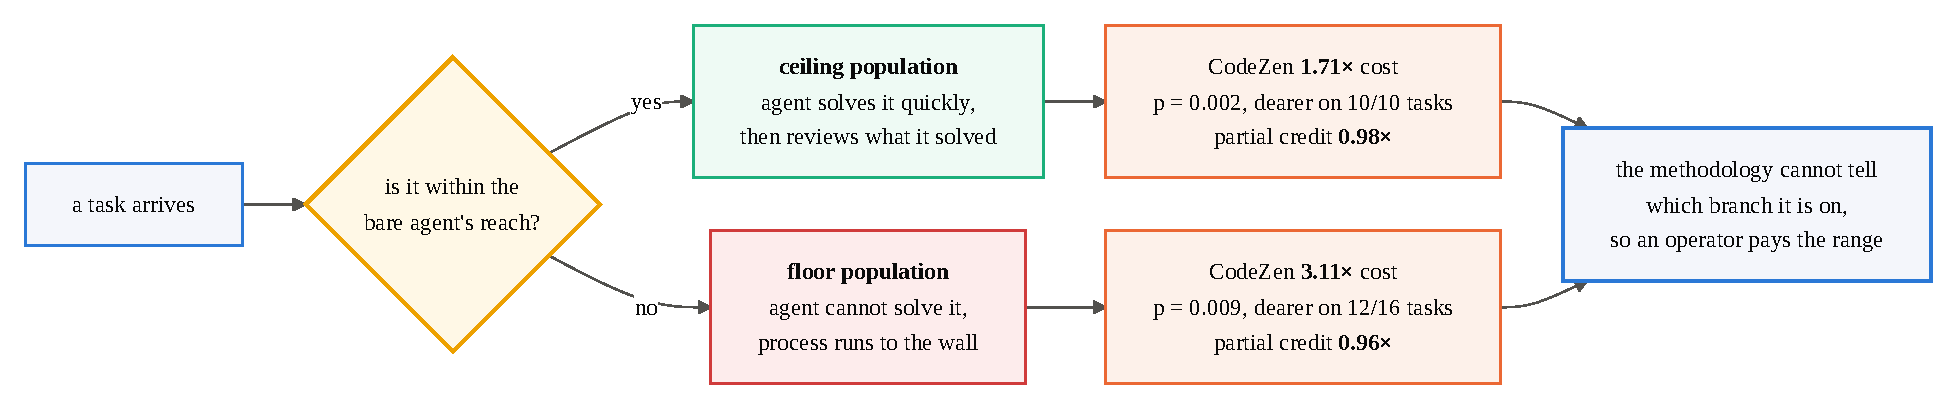
\includegraphics[width=\linewidth]{diagrams/d04-overhead-dynamics.pdf}
\caption{Why the same toolkit produces two multipliers, and why an operator pays the range
rather than either endpoint.}
\label{fig:dynamics}
\end{figure}

\textbf{The smaller run is the stronger evidence.} Ten of ten tasks dearer on four separate
metrics at $p = 0.002$ is a cleaner result than twelve of sixteen at $p = 0.009$, because
there is no task where the effect is absent and no possibility that a runaway trial carries
the mean. CodeZen's per-task cost ratio ranges from $1.01\times$ (\task{sqlite-db-truncate})
to $10.58\times$ (\task{headless-terminal}) in \emph{ceiling}, and from $0.06\times$
(\task{extract-moves-from-video}, where it gave up early) to $16.0\times$
(\task{filter-js-from-html}, where it ran to the wall twice) in \emph{suite}.

\textbf{Cache behaviour rules out an artefact.} Cache hit ratios are effectively identical
across conditions (94.8/94.5/93.4\,\% in \emph{suite}; 96.0/95.8/96.1\,\% in \emph{ceiling}),
and thinking share of output is flat. The extra spend is extra work, not prompt-cache
invalidation.

\textbf{SDD's cost is not the story; SDD's partial credit is.} $1.10$--$1.14\times$ spend is
indistinguishable from baseline in both runs ($p = 0.82$ and $p = 0.28$). But partial credit
lands at $0.833\times$ and $0.818\times$ --- the \emph{same} shortfall in both populations,
independently measured on disjoint task sets. Neither reaches significance, and the
consistency across two disjoint sets is more interesting than either $p$-value.

\subsection{The multiplier is flat in task length; the dollar penalty is not}
\label{sec:cost-length}

\begin{figure}[htbp]
\centering
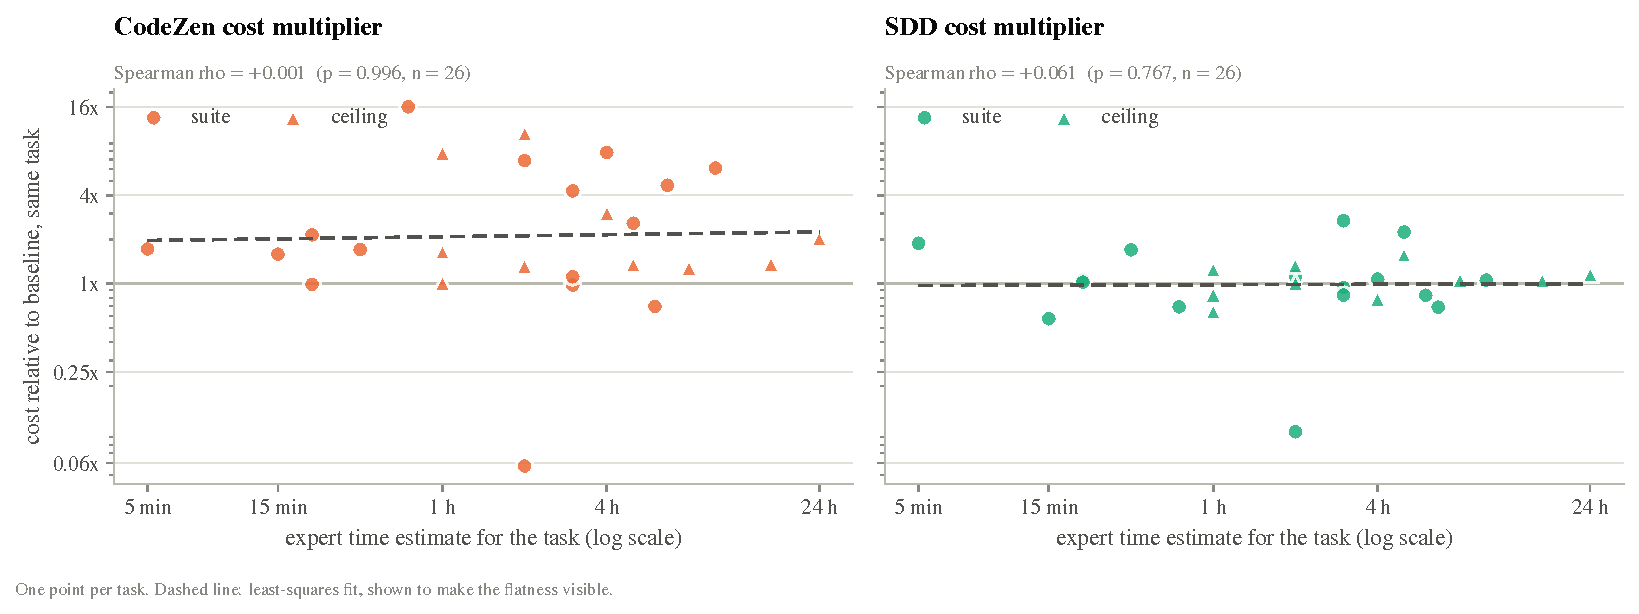
\includegraphics[width=\linewidth]{figures/x07-cost-ratio-vs-length.pdf}
\caption{The cost \emph{multiplier} against expert time estimate, pooled over both runs and
$288\times$ of task length. A Spearman $\rho$ of $+0.001$ against that range is as close to a
flat line as this data can produce: process overhead is proportional, not super-proportional.}
\label{fig:flat}
\end{figure}

Pooled over 26 tasks whose expert estimates span 5 to 1{,}440 minutes:

\begin{center}\small
\begin{tabular}{@{}lrrr@{}}
\toprule
Cost \emph{ratio} vs baseline & vs $\log_{10}$(expert min) & vs declared budget & vs instruction words \\
\midrule
CodeZen & $\rho = +0.001$ ($p = 0.996$) & $-0.006$ ($p = 0.979$) & $+0.324$ ($p = 0.106$) \\
SDD & $+0.061$ ($p = 0.767$) & $+0.129$ ($p = 0.529$) & $+0.254$ ($p = 0.211$) \\
\bottomrule
\end{tabular}
\end{center}

\noindent The absolute dollar penalty does grow, because the base cost grows: baseline
absolute cost against $\log_{10}$(expert min) gives $\rho = +0.696$, $p = 0.0001$ --- the
single strongest correlation in the pooled data. CodeZen's mean overhead is \textbf{\$0.79 per
trial on short-budget tasks ($\le 900$\,s) and \$1.68 on long-budget tasks}: $2.1\times$ the
dollars for the same multiplier.

So the intuition that long tasks are less feasible under a methodology is right, but not for
the reason usually given. The methodology does not become proportionally greedier. A constant
multiplier applied to a larger base is simply a larger bill --- and, as
Section~\ref{sec:clock} shows, the sharper half of the feasibility problem is not the bill at
all.

\subsection{Cost-effectiveness}
\label{sec:costeff}

\begin{table}[htbp]
\centering
\caption{Spend per graded pass and per passing verifier test. The second column pair is the
more robust of the two, because it does not depend on the censoring convention.}
\label{tab:costeff}
\small

\begin{tabular}{@{}llrrrrr@{}}
\toprule
run & condition & graded passes & spend & spend per pass & passing tests & spend per passing test \\
\midrule
suite & baseline & 7 & \$21.87 & \$3.12 & 70 & \$0.312 \\
suite & CodeZen & 9 & \$68.13 & \$7.57 & 72 & \$0.946 \\
suite & SDD & 7 & \$24.89 & \$3.56 & 63 & \$0.395 \\
ceiling & baseline & 17 & \$22.72 & \$1.34 & 49 & \$0.464 \\
ceiling & CodeZen & 13 & \$38.80 & \$2.98 & 50 & \$0.776 \\
ceiling & SDD & 14 & \$24.94 & \$1.78 & 37 & \$0.674 \\
\bottomrule
\end{tabular}

\end{table}

\begin{figure}[htbp]
\centering
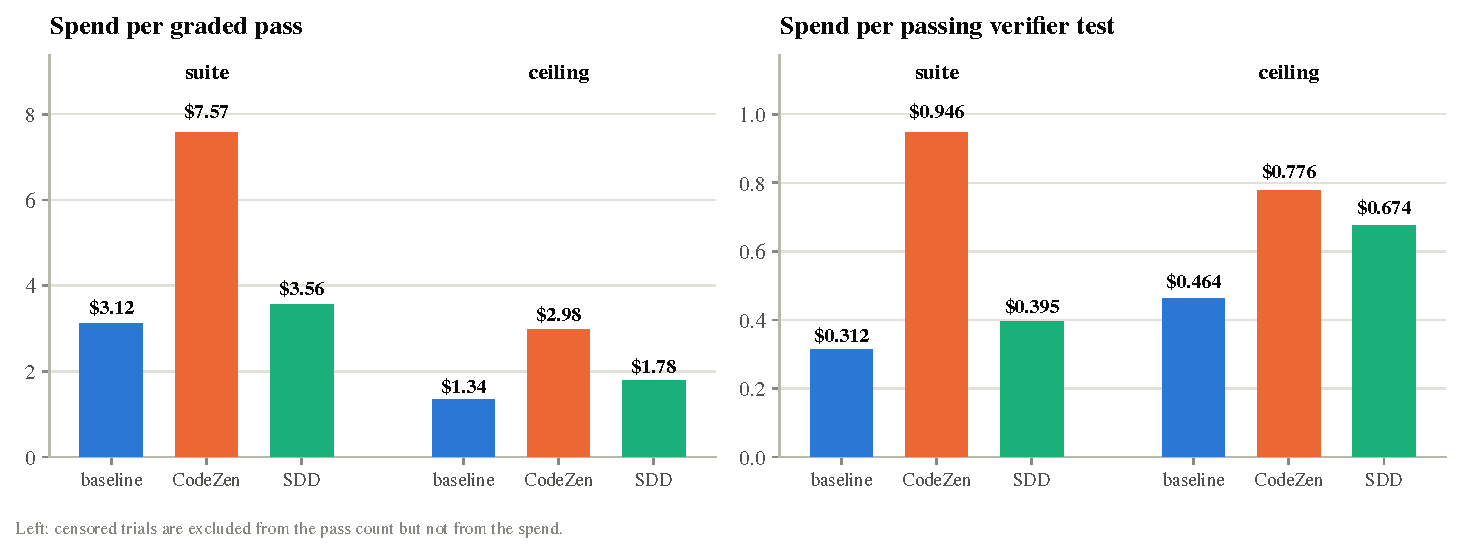
\includegraphics[width=\linewidth]{figures/x12-cost-effectiveness.pdf}
\caption{Cost-effectiveness on both populations. On the \emph{suite} set CodeZen bought two
extra graded passes for \$46.26 --- \$23.13 per marginal success against a baseline unit cost
of \$3.12 --- and those two passes are inside the noise band of
Section~\ref{sec:outcome}. On the \emph{ceiling} set there is no marginal-success framing
available at all: both methodologies produced \emph{fewer} graded passes than baseline while
spending more.}
\label{fig:costeff}
\end{figure}

Baseline is 12\,\% cheaper per pass than SDD and 58\,\% cheaper than CodeZen on the
\emph{suite} set; 25\,\% and 55\,\% cheaper on the \emph{ceiling} set. Per passing verifier
test --- a resolution that does not depend on the censoring convention --- baseline costs
\$0.312, SDD \$0.395 ($+26.6$\,\%) and CodeZen \$0.946 ($+203.2$\,\%) on the \emph{suite}
population.

\clearpage
\section{Results III: the clock is the binding constraint}
\label{sec:clock}

Human software engineering already treats process latency as a first-class cost: the speed of
code review, not only its thoroughness, determines when work reaches users
\citep{kudrjavets2024review}. An autonomous agent sharpens that trade-off, because review and
implementation draw on the \emph{same} bounded execution budget rather than on different
people's calendars. And because that budget is denominated in the same units used to define
agent time horizons \citep{kwa2025horizons}, exhausting it is not an accounting detail but the
event the trial turns on. Whether it actually did is this section's result, not a prior.

\begin{figure}[htbp]
\centering
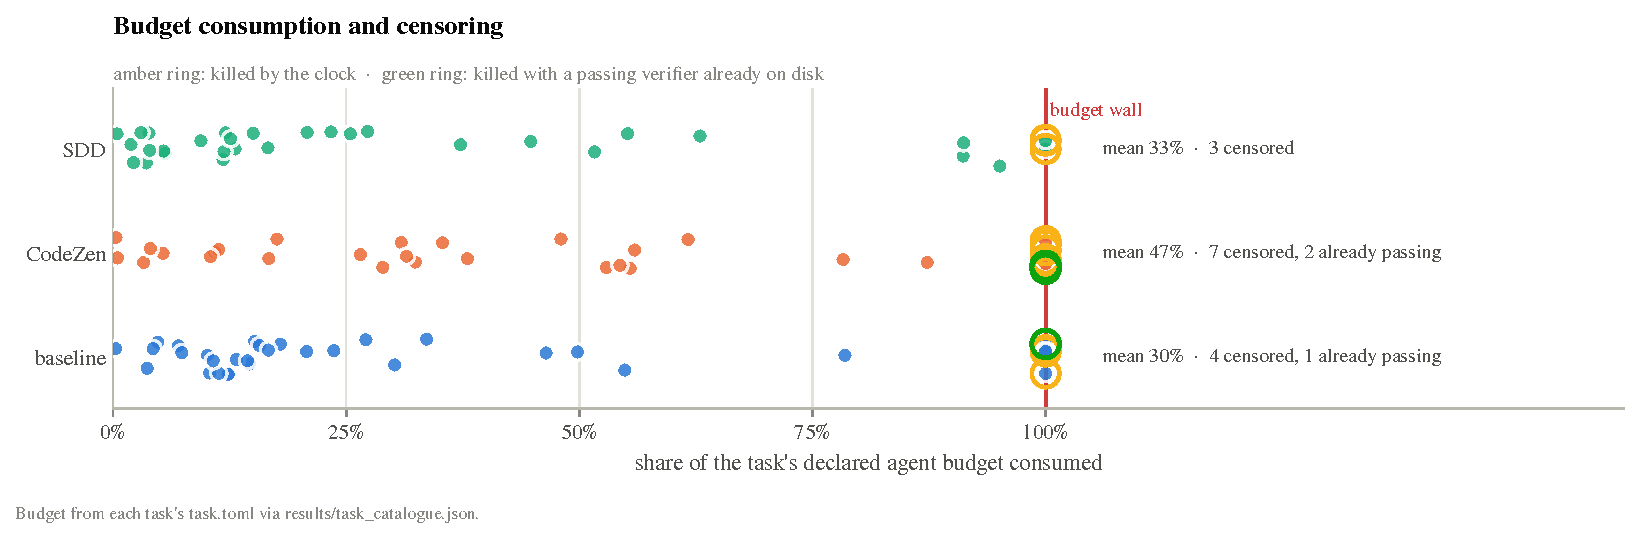
\includegraphics[width=\linewidth]{figures/suite-04-budget.pdf}\\[0.5em]
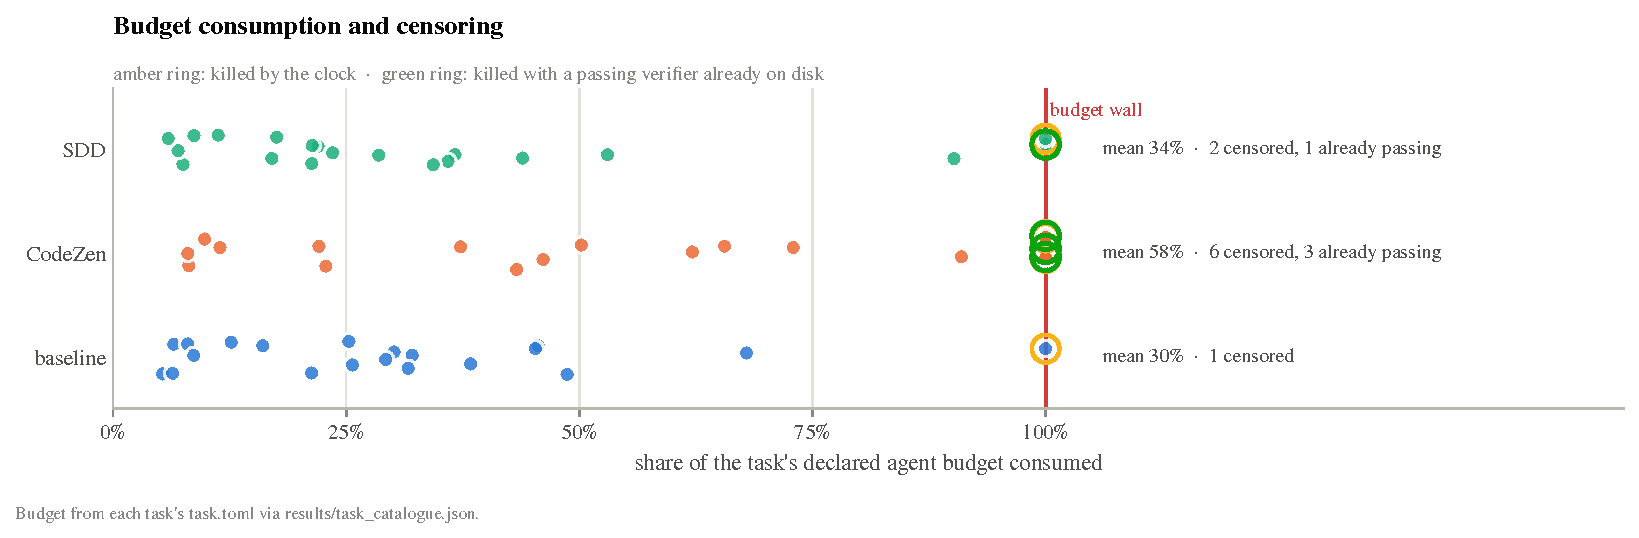
\includegraphics[width=\linewidth]{figures/ceiling-04-budget.pdf}
\caption{Budget consumption and censoring. Each dot is a trial, positioned by the share of
its task's declared agent budget it consumed. Amber rings were killed by the clock; green
rings were killed with a passing verifier already on disk.}
\label{fig:budget}
\end{figure}

\begin{center}\small
\begin{tabular}{@{}llrrrr@{}}
\toprule
Run & Condition & Mean budget & Median & Trials over 75\,\% & Agent timeouts \\
\midrule
\multirow{3}{*}{\emph{suite}}
 & \code{baseline} & 30.2\,\% & 15.4\,\% & 5 & 4 \\
 & \code{codezen-viable} & \textbf{46.8\,\%} & 36.7\,\% & \textbf{9} & \textbf{7} \\
 & \code{sdd} & 33.1\,\% & 15.8\,\% & 6 & 3 \\
\midrule
\multirow{3}{*}{\emph{ceiling}}
 & \code{baseline} & 30.2\,\% & 27.5\,\% & 1 & 1 \\
 & \code{codezen-viable} & \textbf{57.5\,\%} & 56.2\,\% & \textbf{7} & \textbf{6} \\
 & \code{sdd} & 34.3\,\% & 22.8\,\% & 3 & 2 \\
\bottomrule
\end{tabular}
\end{center}

\begin{finding}{The causal chain, fully visible on the ceiling population}
\begin{enumerate}[nosep]
\item CodeZen delegates (2.55 sub-agents per trial against baseline's 0.05) and reviews after
      implementing.
\item That work is real and takes wall-clock, so budget consumption rises $1.90\times$
      ($p = 0.002$, higher on 10 of 10 tasks).
\item On tasks whose budget is tight relative to their size, the extra consumption crosses
      the wall and Harbor kills the agent.
\item Sometimes the work was already done --- 3 of CodeZen's 6 \emph{ceiling} kills scored
      1.0. Sometimes it was not --- \task{torch-pipeline-parallelism} hit 100\,\% of budget on
      both attempts and scored 0 both times, while baseline finished it inside 34\,\%.
\end{enumerate}
\end{finding}

Pooled over 156 trials, the timeout rates are: baseline 5 of 52 (9.6\,\%), SDD 5 of 52
(9.6\,\%), CodeZen \textbf{13 of 52 (25.0\,\%)}.

\subsection{Censoring discards observations that already exist on disk}

\begin{figure}[htbp]
\centering
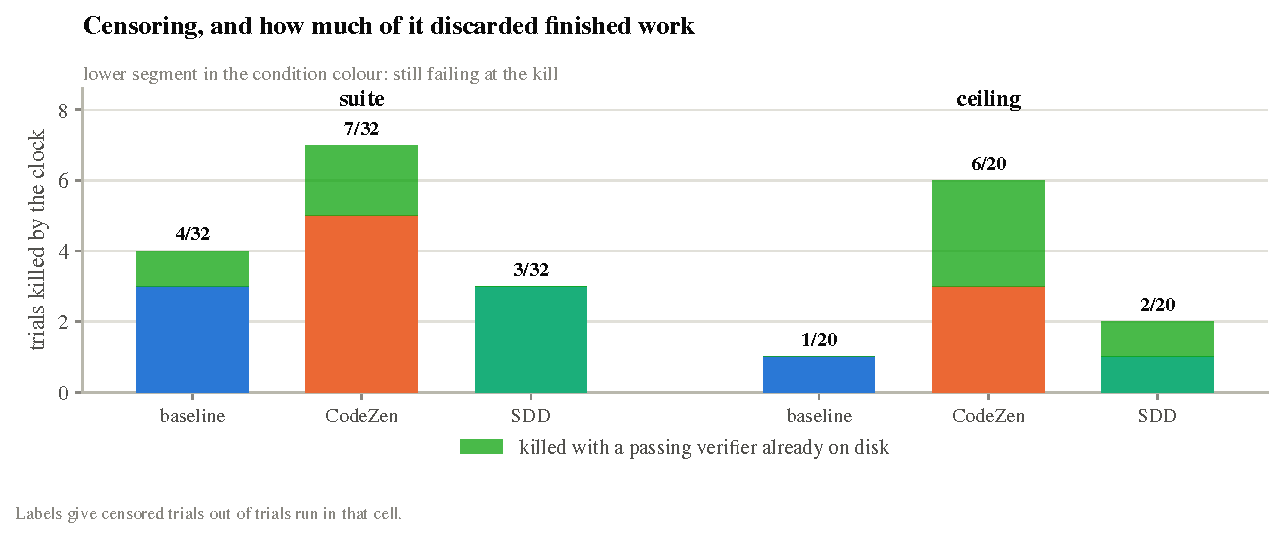
\includegraphics[width=0.92\linewidth]{figures/x08-censoring.pdf}
\caption{Censoring by run and condition, split by what the verifier scored on the workspace
that was killed. Seven of the 23 kills across both runs --- 30.4\,\% --- discarded a solution
that had already passed every test.}
\label{fig:censoring}
\end{figure}

A Harbor timeout is right-censoring in the statistical sense: the trial stopped before the
event of interest, so the observation is a bound rather than a result, and censored
observations carry information that ordinary statistics discard \citep{leung1997censoring}.
The analogy should not be pushed further than that. The censoring mechanism here is
\emph{informative} --- the agent's own behaviour determines whether it reaches the deadline ---
so this is a reason to record what was on disk at the kill, not a licence to apply survival
analysis off the shelf.

Across both runs, 23 trials were censored and \textbf{7 of them scored reward 1.0}: one
baseline and two CodeZen trials in \emph{suite}, three CodeZen and one SDD trial in
\emph{ceiling}. The full list, with the tests each had passed at the kill, is in
Table~\ref{tab:censored} (Appendix~\ref{app:censored}). Reading 3 of
Section~\ref{sec:metrics} already uses those verdicts, which is why it is the column to
prefer: it turns every one of them from a lost observation into a measured one at zero model
cost, and removes the need to choose between dropping a trial and overruling its verifier. An
analysis that adopts it as the primary endpoint has no censoring problem left to reason
about.

\subsection{The post-completion timeout trap}
\label{sec:trap}

The single most illuminating trajectory in the dataset is \task{headless-terminal} under
CodeZen, and it is not a story about difficulty.

\begin{figure}[htbp]
\centering
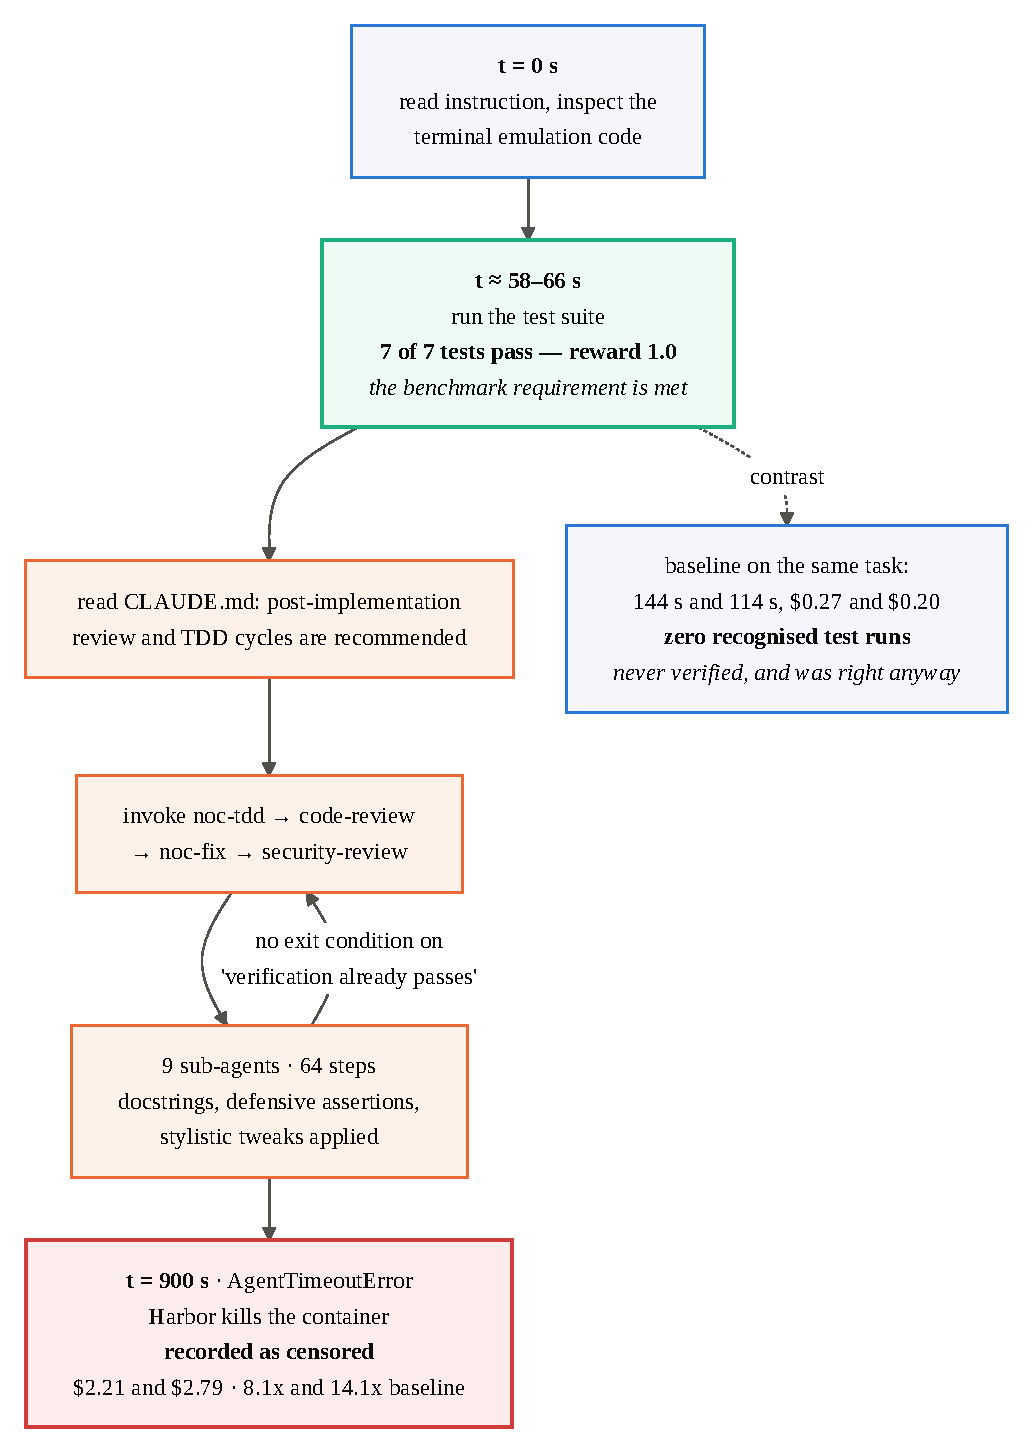
\includegraphics[width=0.80\linewidth]{diagrams/d03-post-completion-trap.pdf}
\caption{\task{headless-terminal} under CodeZen. The functional requirement of the benchmark
was met at 58.4\,s on one attempt and 65.5\,s on the other. The remaining 834 seconds were
ceremonial: nine sub-agents, 64 steps, docstrings and defensive assertions, until Harbor's
hard wall-clock killed the container and the trial was recorded as censored.}
\label{fig:trap}
\end{figure}

Baseline solved the same task in \textbf{144.5\,s and 114.1\,s for \$0.27 and \$0.20},
and --- a detail worth pausing on --- it ran \textbf{zero recognised test invocations} on
either attempt. It edited the terminal emulation code, stopped, and was right anyway. CodeZen
spent \$2.21 and \$2.79, which is $8.1\times$ and $14.1\times$ baseline on the same task, and
both of its attempts were recorded as censored despite scoring reward 1.0.

The contrast is therefore sharper than ``one condition was thorough and one was not''. CodeZen
did the responsible thing --- it ran the tests, and they passed at 65.6\,s and 58.5\,s
according to its own trajectory --- and then kept going for another 834 seconds. Baseline never
verified at all and finished in under two and a half minutes. On this task, the entire cost
difference bought the agent a confirmation it then failed to act on.

\begin{finding}{The architectural lesson}
An autonomous agent operating under a real time or compute budget needs an \textbf{explicit
exit condition}. When verification already succeeds, procedural review skills must be
suppressed or gated behind a strict time-remaining threshold. In human software engineering
thoroughness and peer review are virtues; in an agent with a fixed clock and no termination
gate, thoroughness is a failure mode.

Software-process research has long held that a standardised process should be tuned to the
needs of a specific project rather than applied unchanged \citep{xu2007tailoring}. This
trajectory suggests an autonomous agent needs a strictly more dynamic form of the same idea:
the context that should gate the process is not only the project but the \emph{execution
state} --- whether the artefact already passes --- and the budget still remaining.
Section~\ref{sec:operator} states that as a general claim.
\end{finding}

\noindent The same mechanism, on tasks where the work was \emph{not} already done, is what
produced the \emph{suite} run's $3.11\times$ multiplier: baseline meets a hard barrier ---
a missing shared library, a numerical convergence problem, an obscure binary format --- tries
a few commands and terminates inside about 20 steps and \$0.68. CodeZen treats failure as a
signal to invoke process, calls \code{noc-tdd} to write tests, \code{code-review} to inspect
the non-working code, and \code{noc-fix} to attempt repairs. Because every sub-agent runs the
\emph{same} model, they share the parent's blind spots and cannot conjure domain knowledge
the base model lacks; they return detailed critiques and superficial syntactic suggestions,
and the parent burns steps until the clock expires. On \task{filter-js-from-html} that loop
reached 100\,\% of budget on both attempts at a $16.0\times$ cost ratio, with zero passing
tests.

\subsection{Which tasks are exposed}

The exposure is predicted by the ratio of expert estimate to declared budget rather than by
either quantity alone. Of the six tasks with a ratio at or above $12\times$, CodeZen consumed
100\,\% of budget on \task{adaptive-rejection-sampler}, \task{torch-pipeline-parallelism} and
\task{make-mips-interpreter}, and 93.7\,\% on \task{torch-tensor-parallelism}; baseline
crossed 75\,\% on two of the same six. The correlations are directionally consistent and
underpowered: CodeZen timeouts against the expert/budget ratio give $\rho = +0.304$
($p = 0.131$), SDD $+0.246$ ($p = 0.225$), at $n = 26$ where 80\,\% power needs
$|\rho| \ge 0.53$.

\begin{finding}{The feasibility limit is not the dollar cost --- it is the clock}
The cost multiplier is flat in task length ($\rho = +0.001$). The budget multiplier is not
flat in exposure: it is $1.90\times$, and on tasks whose budget is tight relative to their
size it converts directly into kills. An operator running under a real deadline faces the
same arithmetic Harbor imposes.
\end{finding}

\clearpage
\section{Results IV: behaviour and adherence}
\label{sec:behaviour}

\subsection{What the agent actually did differently}

\begin{table}[htbp]
\centering
\caption{Behavioural profile, per-trial means, both runs. Shell commands are bucketed by
pattern rather than parsed, so ``verification commands'' should be read as a comparison
between conditions on one corpus, not as an absolute count.}
\label{tab:behaviour}
\small

\begin{tabular}{@{}lrrrrrr@{}}
\toprule
 & \multicolumn{3}{c}{\textbf{suite}} & \multicolumn{3}{c}{\textbf{ceiling}} \\
\cmidrule(lr){2-4}\cmidrule(lr){5-7}
per-trial mean & baseline & CodeZen & SDD & baseline & CodeZen & SDD \\
\midrule
agent steps & 21.9 & 48.0 & 24.8 & 26.0 & 42.9 & 28.2 \\
tool calls & 23.4 & 51.3 & 25.0 & 26.8 & 47.0 & 30.9 \\
file edits / writes & 1.97 & 6.41 & 3.44 & 3.20 & 4.75 & 4.30 \\
verification commands & 0.56 & 3.56 & 0.66 & 0.30 & 1.65 & 0.00 \\
sub-agents spawned & 0.03 & 2.62 & 0.00 & 0.05 & 2.55 & 0.05 \\
file reads & 4.22 & 10.31 & 3.66 & 2.95 & 6.85 & 4.40 \\
wrote a test file & 9.4\% & 34.4\% & 3.1\% & 10.0\% & 25.0\% & 0.0\% \\
tool results with an error & 10.2\% & 12.9\% & 9.7\% & 13.1\% & 16.9\% & 10.9\% \\
cache hit ratio & 94.8\% & 94.5\% & 93.4\% & 96.0\% & 95.8\% & 96.1\% \\
thinking share of output & 59.5\% & 59.2\% & 60.7\% & 67.2\% & 65.7\% & 65.4\% \\
\bottomrule
\end{tabular}

\end{table}

\begin{figure}[htbp]
\centering
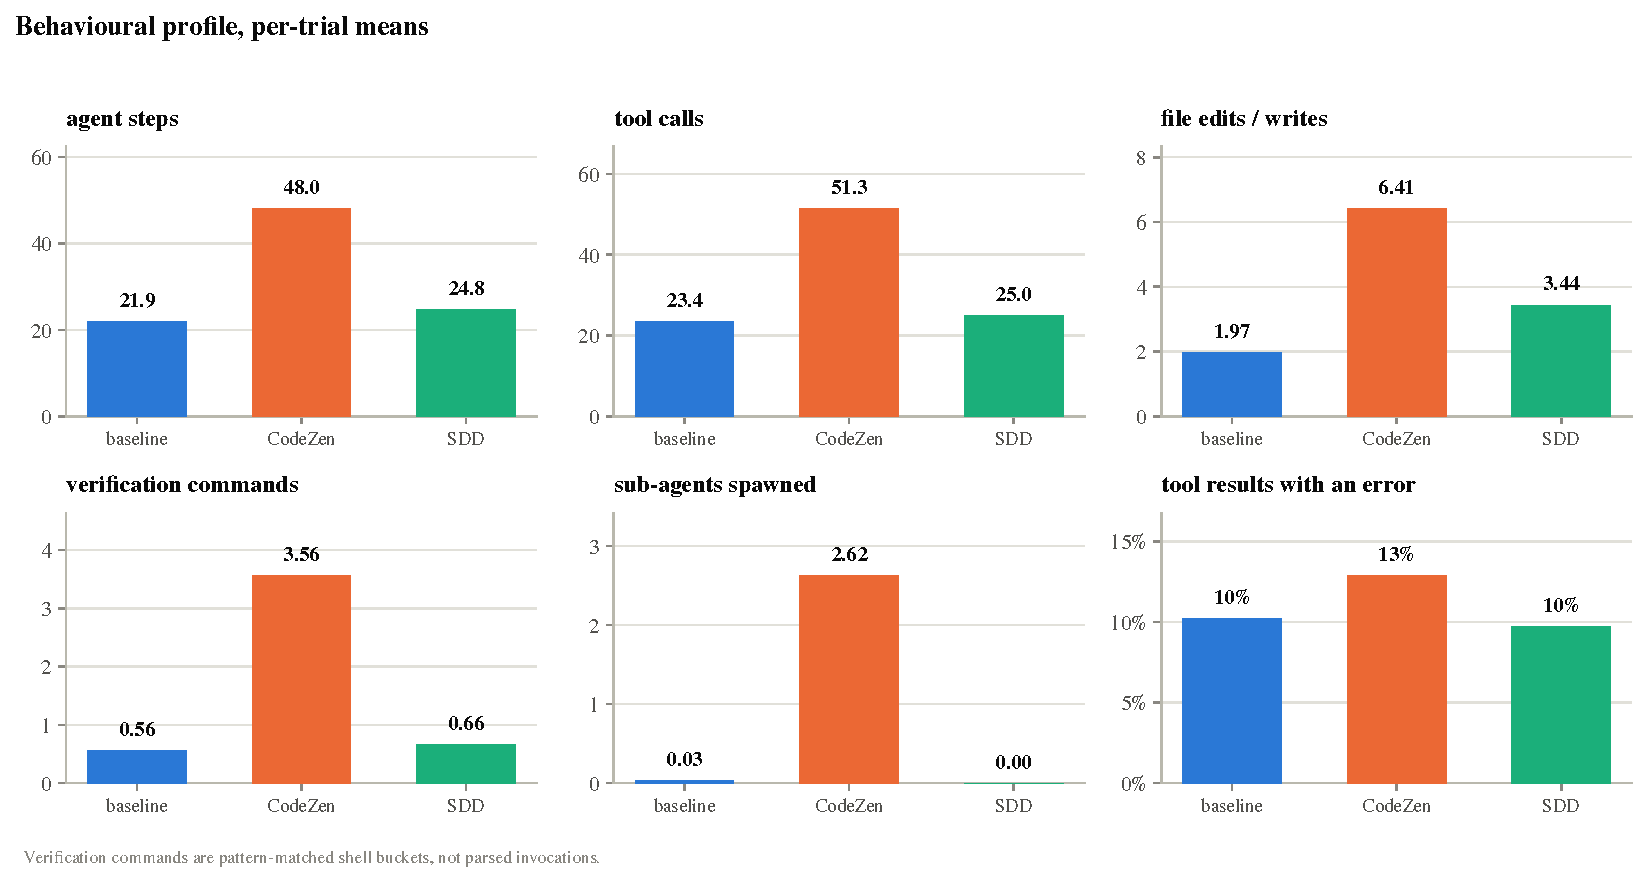
\includegraphics[width=\linewidth]{figures/suite-05-behaviour.pdf}\\[0.4em]
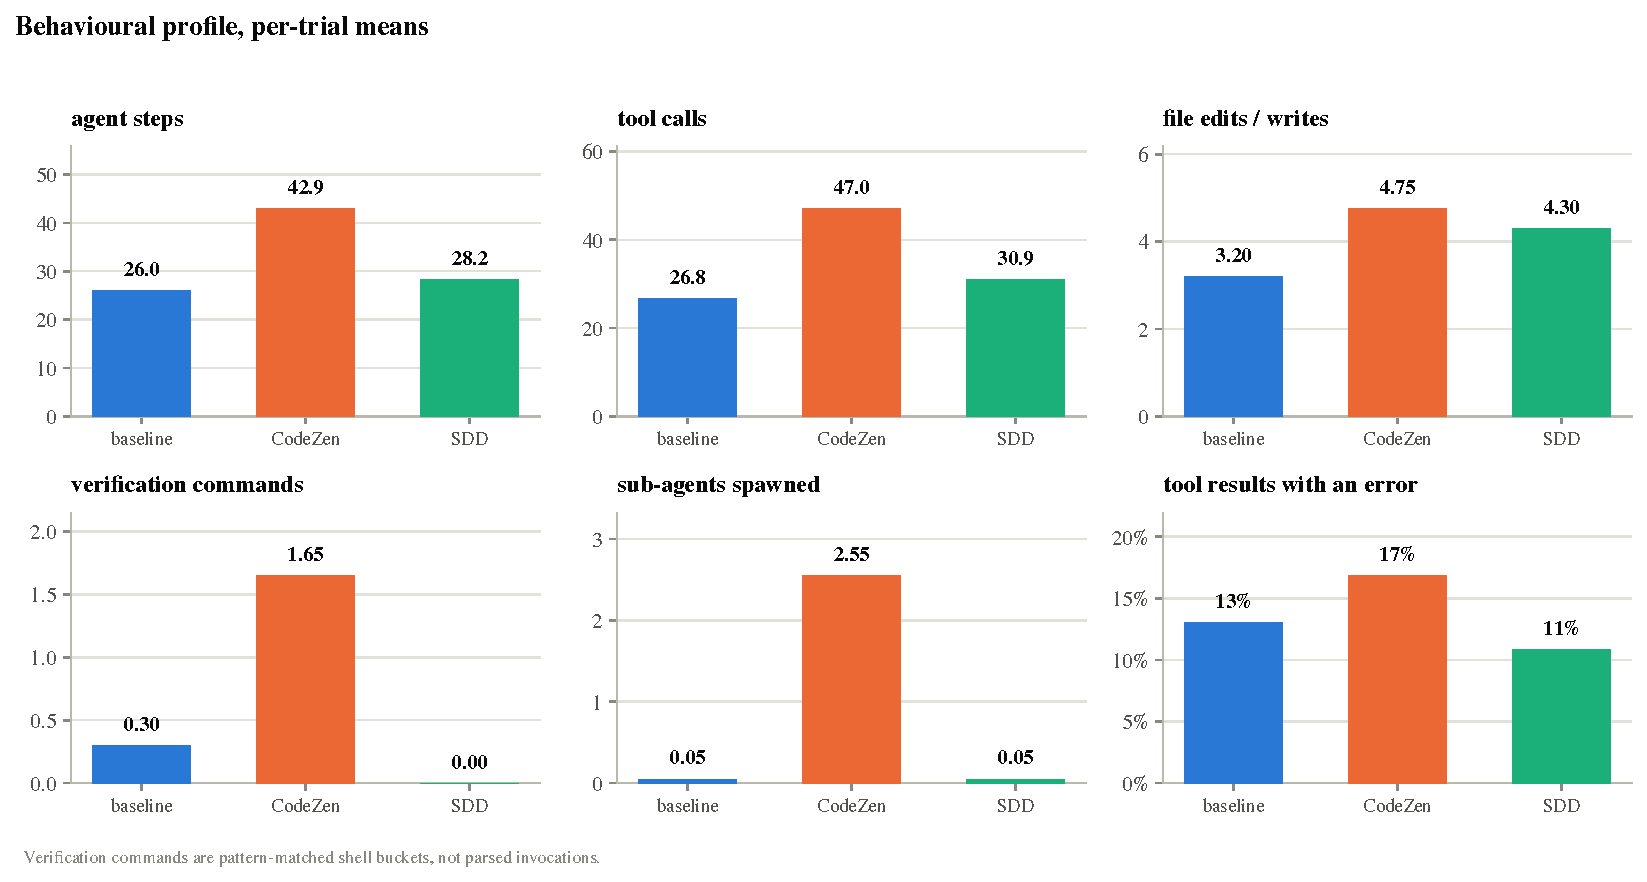
\includegraphics[width=\linewidth]{figures/ceiling-05-behaviour.pdf}
\caption{Behavioural profiles. Top: \emph{suite}. Bottom: \emph{ceiling}. CodeZen's signature
is stable across two disjoint populations --- more reading, more verifying, and above all
more delegating --- and SDD's is close to invisible on both.}
\label{fig:behaviour}
\end{figure}

Three observations carry the section.

\paragraph{CodeZen delegates, and that is its whole cost signature.} 84 sub-agent spawns
across its 32 \emph{suite} trials against 1 for baseline and 0 for SDD; 51 across its 20
\emph{ceiling} trials against 1 for baseline. Each sub-agent inherits prompt context and
produces its own thinking and output tokens, which accounts for the bulk of the step and
token overhead in Section~\ref{sec:cost}. It is also invisible to the cell-level report,
which has no delegation column. Whether decomposition into multiple agents buys capability or
mostly coordination overhead is an open question in its own right, and the counter-position is
instructive: a deliberately simple
localise--repair--validate pipeline has been shown competitive with elaborate agent
scaffolding on repository-level tasks \citep{xia2024agentless}. Here the sub-agents run the
\emph{same} model as the parent, so they inherit its blind spots along with its context.

\paragraph{CodeZen verifies far more, and it does not help.} The expectation under test here
is a well-supported one. Systematic review associates test-driven development with better
internal and external quality while finding its productivity effect mixed or negative
\citep{bissi2016tdd}, and a large industry experiment likewise found quality gains without a
productivity gain \citep{tosun2017industry}. What follows is therefore not evidence that
testing is harmful. It is a question about whether that trade-off survives translation into
an agent with a fixed execution budget and no access to the grading oracle.

3.56 verification commands per trial against baseline's 0.56 in \emph{suite} --- a
$6.3\times$ increase, $p = 0.046$ --- and 1.65 against 0.30 in \emph{ceiling}. It wrote a dedicated test file in 34.4\,\% of
\emph{suite} trials against baseline's 9.4\,\%. This is the one place the toolkit does exactly
what it advertises, and partial credit still came out $0.96\times$ baseline.

\begin{finding}{A hypothesis for why more testing did not mean more correctness}
This mechanism is \emph{proposed}, not measured. What the data establishes is the disconnect
between verification activity and verified outcome; what follows is our account of it.

In an autonomous benchmark the verifier is an external oracle the agent cannot see. When an
agent writes its own tests it tests against its \emph{own} interpretation of the problem: if
it has misread an edge case, it encodes the misreading in a test, runs it, sees green, and
believes the solution is correct. The external verifier then tests the actual edge case and
fails it. On this reading, ungrounded test-driven development produces \textbf{false
confidence}, and testing is only as good as the specification it validates against.

Two things make it plausible rather than merely available. Agents are a distinct class of end
user, with needs and failure modes that differ from a human developer's
\citep{yang2024sweagent}, and interactive agent evaluation repeatedly identifies weak
long-horizon reasoning and instruction following among the dominant failure modes
\citep{liu2024agentbench}. Section~\ref{sec:recommendations} names the instrument that would
settle it: log a ``mock misalignment'' event whenever the agent's own suite passes and the
official verifier does not.
\end{finding}

\paragraph{SDD is behaviourally almost invisible --- except where it points the wrong way.}
Steps $1.13\times$, tool calls $1.07\times$, wall-clock $0.99\times$, zero sub-agents in
\emph{suite}. Its only distinct positive signal is $1.75\times$ the file edits. And in the
\emph{ceiling} run it ran \textbf{zero} recognised verification commands across 20 trials,
against baseline's 0.30 and CodeZen's 1.65 --- for a methodology that ships an
\code{sdd-verify} skill and invoked it in two of its four skill-using trials. That lines up
with the partial-credit shortfall: SDD satisfied 68.5\,\% of verifier tests against
baseline's 90.7\,\%, and checked its work less than the bare agent did.

The caveat matters more here than anywhere else in the paper: verification done inline in a
heredoc is invisible to the pattern bucket, so 0.00 means ``no recognised test invocation'',
not ``nothing was checked''. But the same bucket credits baseline with 0.30 and CodeZen with
1.65 on the same corpus, so the \emph{comparison} stands even if the absolute count
understates.

\subsection{Availability is total; adherence is rare}
\label{sec:adherence}

\begin{table}[htbp]
\centering
\caption{The adherence funnel, under the strict definition: a \code{Skill} tool call whose
skill name is one the variant installed. Every toolkit skill registered in every one of the
104 toolkit trials, and preflight proved every instruction file present.}
\label{tab:adherence}
\small

\begin{tabular}{@{}lrrrrrr@{}}
\toprule
 & \multicolumn{3}{c}{\textbf{suite} (32 trials each)} & \multicolumn{3}{c}{\textbf{ceiling} (20 trials each)} \\
\cmidrule(lr){2-4}\cmidrule(lr){5-7}
 & baseline & CodeZen & SDD & baseline & CodeZen & SDD \\
\midrule
skills shipped & 0 & 4 & 7 & 0 & 4 & 7 \\
registered by the CLI & 0 & 4 & 7 & 0 & 4 & 7 \\
named an instruction file in its output & 0 & 14 & 3 & 0 & 8 & 7 \\
opened one with \texttt{Read} or \texttt{cat} & 0 & 10 & 0 & 0 & 5 & 4 \\
invoked a toolkit skill & 0 & 12 & 7 & 0 & 7 & 4 \\
toolkit \texttt{Skill} calls in total & 0 & 28 & 27 & 0 & 17 & 13 \\
\bottomrule
\end{tabular}

\end{table}

\begin{figure}[htbp]
\centering
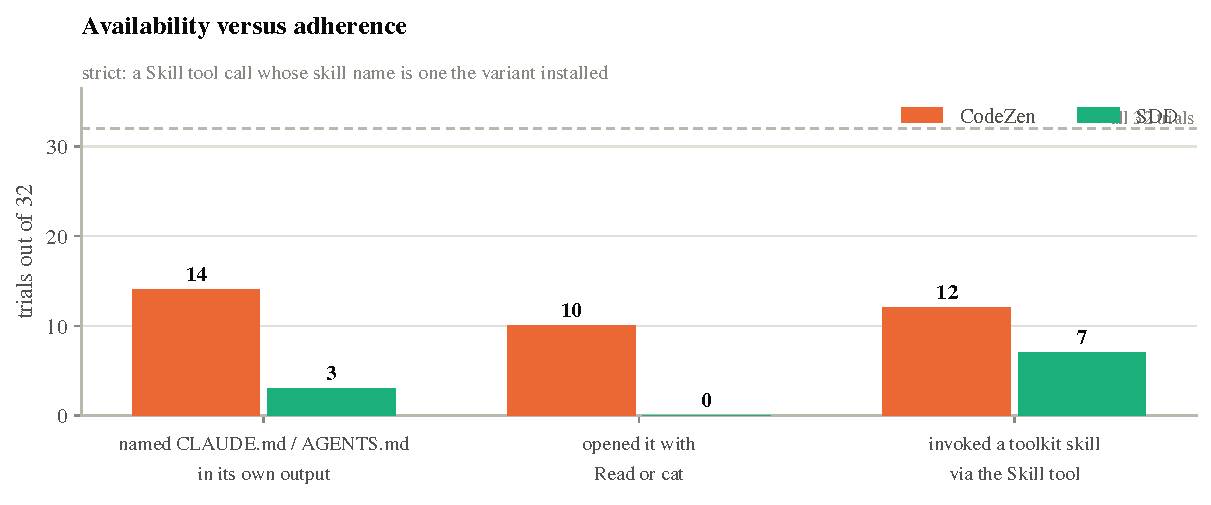
\includegraphics[width=0.49\linewidth]{figures/suite-06-adherence.pdf}
\hfill
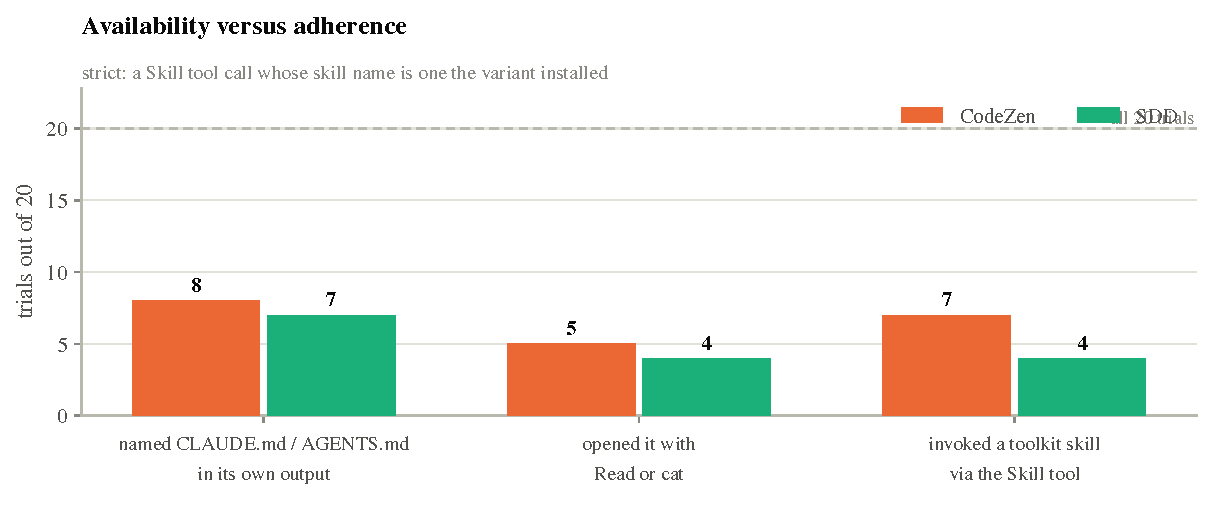
\includegraphics[width=0.49\linewidth]{figures/ceiling-06-adherence.pdf}
\caption{Availability versus adherence. Left: \emph{suite}. Right: \emph{ceiling}. The dashed
line is all trials in the cell. Registration reached 100\,\% everywhere; invocation reached
20--38\,\%.}
\label{fig:adherence}
\end{figure}

\begin{finding}{Whatever these runs measured, it was not a methodology being followed}
Across both runs, \textbf{74 of 104 toolkit trials (71\,\%) invoked no toolkit skill at all}.
CodeZen invoked one in 12 of 32 \emph{suite} trials (38\,\%) and 7 of 20 \emph{ceiling} trials
(35\,\%); SDD in 7 of 32 (22\,\%) and 4 of 20 (20\,\%). The comparison under test is
therefore not ``method versus no method'' but ``a repository containing a method, mostly
unused, versus a bare task''.
\end{finding}

\noindent ``Opened an instruction file'' is a weak proxy for Claude Code specifically: it
loads a project \code{CLAUDE.md} silently into its system prompt, so an agent has no reason to
open a file it has already been given. SDD's zero reads and three mentions in \emph{suite} are
therefore not evidence of absence. Its seven skill-invoking trials are.

\subsection{Every trial that invoked a skill}

\begin{table}[htbp]
\centering
\caption{All 30 trials across both runs that invoked a toolkit skill, with the invocation
order, sub-agents spawned, reward, budget consumed and cost. ``censored'' marks a Harbor
timeout, which for four of these rows arrived \emph{after} the verifier would have scored 1.0.}
\label{tab:skilltrials}
\scriptsize
\resizebox{\linewidth}{!}{
\begin{tabular}{@{}llllrrrrl@{}}
\toprule
run & task & condition & skills invoked, in order & sub & reward & budget & cost & outcome \\
\midrule
suite & adaptive-rejection-sampler & CodeZen & \texttt{\footnotesize noc-tdd, code-review, noc-fix} & 6 & 1.0 & 100\% & \$2.87 & pass, censored \\
suite & adaptive-rejection-sampler & CodeZen & \texttt{\footnotesize noc-tdd, code-review} & 6 & 0.0 & 100\% & \$2.75 & fail, censored \\
suite & cancel-async-tasks & CodeZen & \texttt{\footnotesize noc-tdd} & 0 & 1.0 & 11\% & \$0.24 & pass \\
suite & cancel-async-tasks & CodeZen & \texttt{\footnotesize noc-tdd, code-review} & 6 & 1.0 & 78\% & \$2.48 & pass \\
suite & filter-js-from-html & CodeZen & \texttt{\footnotesize noc-tdd, code-review, security-review} & 9 & 0.0 & 100\% & \$6.74 & fail, censored \\
suite & filter-js-from-html & CodeZen & \texttt{\footnotesize noc-tdd, code-review, security-review} & 9 & 0.0 & 100\% & \$6.30 & fail, censored \\
suite & sam-cell-seg & CodeZen & \texttt{\footnotesize code-review, security-review} & 9 & 0.0 & 27\% & \$6.11 & fail \\
suite & sam-cell-seg & CodeZen & \texttt{\footnotesize code-review, security-review} & 9 & 0.0 & 31\% & \$6.84 & fail \\
suite & torch-tensor-parallelism & CodeZen & \texttt{\footnotesize noc-tdd, code-review, security-review} & 9 & 0.0 & 87\% & \$3.14 & fail \\
suite & torch-tensor-parallelism & CodeZen & \texttt{\footnotesize noc-tdd, code-review} & 6 & 1.0 & 100\% & \$2.62 & pass, censored \\
suite & video-processing & CodeZen & \texttt{\footnotesize noc-tdd, code-review} & 6 & 0.0 & 29\% & \$4.23 & fail \\
suite & video-processing & CodeZen & \texttt{\footnotesize noc-tdd, code-review, security-review} & 9 & 0.0 & 56\% & \$7.61 & fail \\
suite & adaptive-rejection-sampler & SDD & \texttt{\footnotesize sdd-specify, sdd-plan, sdd-tasks, sdd-analyze, sdd-implement, sdd-verify} & 0 & 0.0 & 91\% & \$1.72 & fail \\
suite & adaptive-rejection-sampler & SDD & \texttt{\footnotesize sdd-specify, sdd-clarify, sdd-plan, sdd-tasks, sdd-analyze, sdd-implement, sdd-verify} & 0 & 1.0 & 91\% & \$1.79 & pass \\
suite & filter-js-from-html & SDD & \texttt{\footnotesize sdd-specify, sdd-clarify} & 0 & 0.0 & 5\% & \$0.19 & fail \\
suite & sam-cell-seg & SDD & \texttt{\footnotesize sdd-specify, sdd-clarify} & 0 & 0.0 & 2\% & \$0.28 & fail \\
suite & sam-cell-seg & SDD & \texttt{\footnotesize sdd-specify, sdd-clarify, sdd-plan, sdd-tasks, sdd-analyze, sdd-implement, sdd-verify} & 0 & 0.0 & 9\% & \$1.96 & fail \\
suite & video-processing & SDD & \texttt{\footnotesize sdd-specify} & 0 & 0.0 & 23\% & \$1.50 & fail \\
suite & video-processing & SDD & \texttt{\footnotesize sdd-specify, sdd-clarify} & 0 & 0.0 & 3\% & \$0.25 & fail \\
ceiling & headless-terminal & CodeZen & \texttt{\footnotesize noc-tdd, code-review, noc-fix, security-review} & 9 & 1.0 & 100\% & \$2.21 & pass, censored \\
ceiling & headless-terminal & CodeZen & \texttt{\footnotesize noc-tdd, code-review, security-review} & 9 & 1.0 & 100\% & \$2.79 & pass, censored \\
ceiling & make-mips-interpreter & CodeZen & \texttt{\footnotesize code-review, noc-fix} & 6 & 0.0 & 100\% & \$5.85 & fail, censored \\
ceiling & make-mips-interpreter & CodeZen & \texttt{\footnotesize noc-tdd, code-review} & 6 & 1.0 & 100\% & \$4.42 & pass, censored \\
ceiling & pypi-server & CodeZen & \texttt{\footnotesize noc-tdd, code-review, security-review} & 9 & 1.0 & 50\% & \$1.80 & pass \\
ceiling & torch-pipeline-parallelism & CodeZen & \texttt{\footnotesize code-review} & 6 & 0.0 & 100\% & \$1.63 & fail, censored \\
ceiling & torch-pipeline-parallelism & CodeZen & \texttt{\footnotesize noc-tdd, code-review} & 6 & 0.0 & 100\% & \$1.65 & fail, censored \\
ceiling & headless-terminal & SDD & \texttt{\footnotesize sdd-specify, sdd-clarify} & 0 & 0.0 & 11\% & \$0.21 & fail \\
ceiling & make-mips-interpreter & SDD & \texttt{\footnotesize sdd-specify, sdd-analyze, sdd-verify} & 1 & 0.0 & 90\% & \$3.45 & fail \\
ceiling & schemelike-metacircular-eval & SDD & \texttt{\footnotesize sdd-specify, sdd-plan, sdd-tasks, sdd-analyze, sdd-implement, sdd-verify} & 0 & 0.0 & 53\% & \$3.20 & fail \\
ceiling & torch-pipeline-parallelism & SDD & \texttt{\footnotesize sdd-specify, sdd-clarify} & 0 & 0.0 & 17\% & \$0.28 & fail \\
\bottomrule
\end{tabular}
}
\end{table}

Two patterns in Table~\ref{tab:skilltrials} deserve names.

\paragraph{CodeZen's \code{noc-tdd} drives implementation; the review skills follow it.}
\textbf{Ten} of 12 \emph{suite} CodeZen trials and 5 of 7 \emph{ceiling} ones start with
\code{noc-tdd}, and \code{code-review} and \code{security-review} appear \emph{after} the work
rather than as a method for doing it.
Where the full chain ran to the budget wall the cost was $4.3\times$ and $16.0\times$
baseline.

The ordering is worth keeping in view, because the human TDD literature has itself struggled
to separate the benefit of writing tests \emph{first} from the benefit of working in short,
tightly verified cycles \citep{fucci2017dissection}. A toolkit that invokes a test-first skill
and then implements in one pass is not obviously practising the thing the evidence supports.

\paragraph{SDD's chain either runs completely or aborts at step two.} Five trials across both
runs stop after \code{sdd-specify} and \code{sdd-clarify} having consumed 2.2--17.0\,\% of the
budget, and a sixth stops after \code{sdd-specify} alone at 23.4\,\%: the agent opened the
process, produced a specification, and did not follow it.
Producing the specification consumed context and steps without bringing the agent closer to
executable code; sensing time pressure, it abandoned the remaining stages and reverted to
unassisted coding --- with cluttered context and lost time. The only SDD success anywhere in
the table is one attempt of \task{adaptive-rejection-sampler}, whose sibling attempt ran a
nearly identical chain and failed.

\subsection{Does invoking the methodology predict failure?}
\label{sec:selection}

Pooled over both runs, of the 30 trials that invoked a toolkit skill, 30.0\,\% passed. Of the
toolkit trials that invoked nothing, 54.1\,\% passed. In the \emph{ceiling} run the contrast
is starker: 4 of 11 skill-using trials passed against a run-wide 77--93\,\%.

\begin{finding}{Selection and effect cannot be separated in this design --- and both are supported}
The \textbf{distress hypothesis}: when the agent immediately grasps a solution it edits files
and runs commands, ignoring the skills directory; when it is stuck, confused by test output,
or facing something that looks unusually hard, it reaches for the documented process as a
fallback. On that reading the low pass rate of skill-using trials is an artefact of the tasks
those trials were on.

The \textbf{consumption hypothesis}: invoking the chain consumes the budget that would have
solved the task. This is supported independently by the censoring data --- every
\emph{ceiling} trial that invoked a skill and hit 100\,\% of budget is in
Table~\ref{tab:skilltrials}.

Section~\ref{sec:length} adds evidence for the first: SDD's invocation rate rises with task
size, which is self-gating rather than harness suppression. But only a design that
\emph{randomises} invocation can separate the two, and no run in this sequence has done that.
\end{finding}

\clearpage
\section{Results V: the length hypothesis}
\label{sec:length}

Human expert completion time is the axis on which modern agent evaluation defines a
task-completion horizon --- the task duration at which an agent is predicted to succeed with a
given reliability \citep{kwa2025horizons} --- so it is both the natural predictor for this
hypothesis and the one the benchmark supplies.

The hypothesis that motivated the pooled analysis was stated informally before the runs:

\begin{quote}\small
``Longer horizon tasks are a bit less feasible on account of the cost, but that hypothesis
about methodology enforcement being more useful at higher task length feels worth exploring.''
\end{quote}

That is two claims, and both are testable on the pooled 26 tasks, whose expert estimates span
5 to 1{,}440 minutes --- a $288\times$ range --- with 10 tasks carrying Terminal-Bench's own
\code{long-horizon} axis.

\subsection{Claim 1 --- cost makes long tasks less feasible}

\textbf{Supported in absolute terms, refuted as a multiplier.} This is
Section~\ref{sec:cost-length}: the ratio is flat at $\rho = +0.001$, the absolute overhead
grows because the base grows, and the binding constraint is the clock rather than the bill.

\subsection{Claim 2 --- methodology is more useful at higher task length}

\textbf{Not supported, and not powered to reject.} The hypothesis predicts that the
methodology's outcome advantage grows with task length. Three outcome measures at increasing
resolution, against two length measures:

\begin{figure}[htbp]
\centering
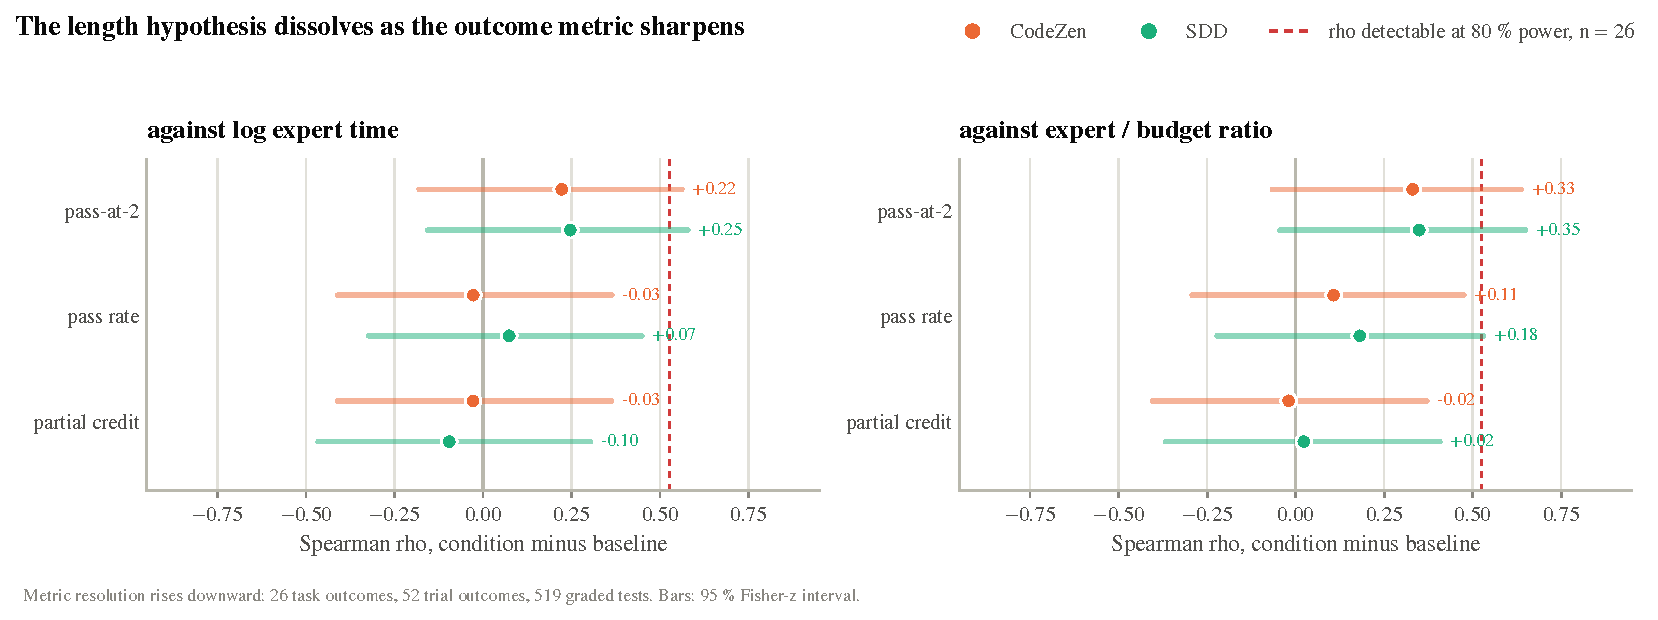
\includegraphics[width=\linewidth]{figures/x10-length-dissolution.pdf}
\caption{The length effect as a function of metric resolution. Reading downward, the outcome
measure sharpens from 26 binary task outcomes to 52 binary trial outcomes to 519 graded
verifier tests. A real effect should sharpen with the instrument. This one dissolves --- and
for CodeZen against expert time it turns faintly negative.}
\label{fig:dissolution}
\end{figure}

There is a weak positive lean in the predicted direction, and \emph{only in the coarsest
metric}: $\Delta$ pass-at-2 against the expert/budget ratio gives $\rho = +0.330$ (CodeZen,
$p = 0.099$) and $+0.349$ (SDD, $p = 0.081$) --- the largest effects available, both just
outside significance, both at roughly 35--40\,\% power. The same comparison on pass
\emph{rate}, which uses both attempts rather than the best one, drops to $+0.107$ and
$+0.181$. On partial credit --- 519 graded test outcomes rather than 26 binary ones --- it is
indistinguishable from zero.

\begin{finding}{The signature of noise in a coarse metric}
A real effect should sharpen as the metric sharpens. This one dissolves. The honest conclusion
is that the data does not support the hypothesis and is not powered to reject it.
\end{finding}

\noindent Terminal-Bench's own \code{long-horizon} axis says the same and adds something:

\begin{table}[htbp]
\centering
\caption{The \code{long-horizon} axis split (expert estimate at or above four hours), pooled
over 26 tasks. On every finer-grained outcome measure both methodologies do \emph{worse} on
long-horizon tasks than on short ones --- the opposite direction to the hypothesis.}
\label{tab:longhorizon}
\small

\begin{tabular}{@{}lrrr@{}}
\toprule
 & long-horizon ($n = 10$) & short ($n = 16$) & \multicolumn{1}{c}{Mann--Whitney $p$} \\
\midrule
$\Delta$ pass-at-2, CodeZen & $+0.100$ & $+0.062$ & 0.858 \\
$\Delta$ pass-at-2, SDD & $+0.000$ & $+0.000$ & 1.000 \\
$\Delta$ pass rate, CodeZen & $-0.050$ & $+0.094$ & 0.391 \\
$\Delta$ pass rate, SDD & $-0.100$ & $-0.031$ & 0.832 \\
$\Delta$ partial credit, CodeZen & $-0.057$ & $+0.004$ & 0.389 \\
$\Delta$ partial credit, SDD & $-0.182$ & $-0.080$ & 0.303 \\
cost ratio, CodeZen & $+3.099$ & $+3.737$ & 0.693 \\
cost ratio, SDD & $+1.154$ & $+1.107$ & 0.732 \\
toolkit skill calls per attempt, CodeZen & $+1.050$ & $+0.750$ & 0.469 \\
toolkit skill calls per attempt, SDD & $+1.150$ & $+0.531$ & 0.093 \\
\bottomrule
\end{tabular}

\end{table}

The differences are not significant, but they are consistent across two metrics and two
toolkits, and they point the wrong way. SDD's partial-credit deficit on long-horizon tasks is
$-0.182$ against $-0.080$ on short ones: its worst performance is exactly where its own
documentation claims it should be strongest.

\subsection{The most interesting result: the toolkits behave as if the hypothesis were true}

\begin{figure}[htbp]
\centering
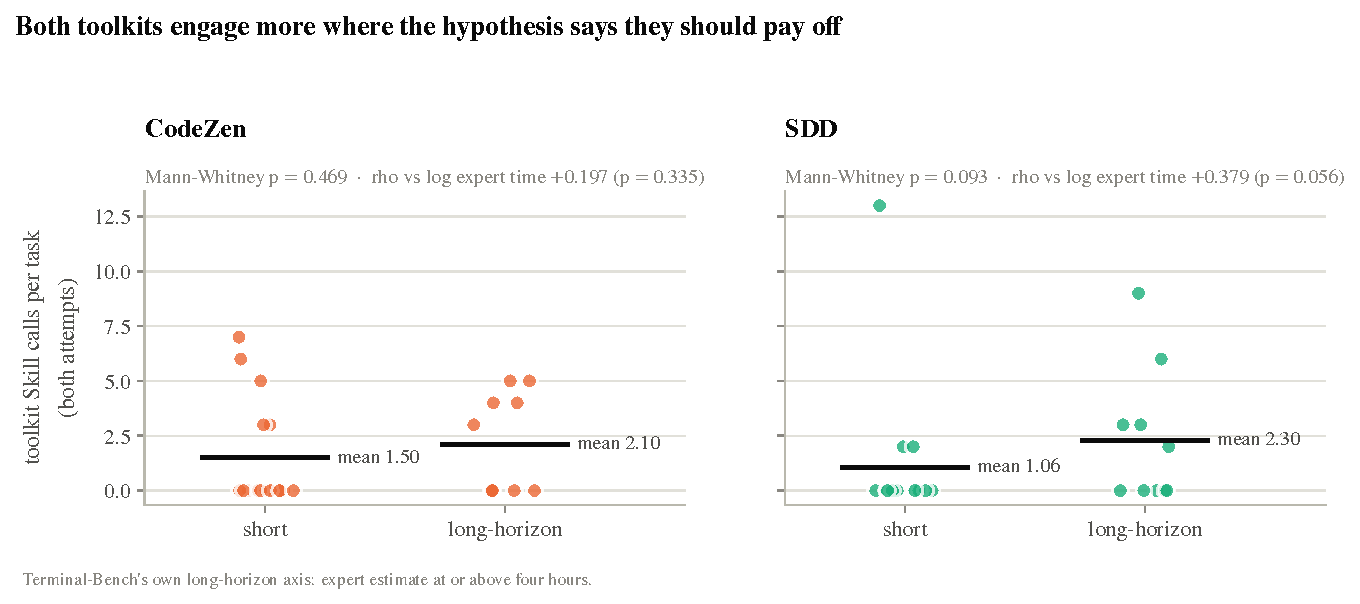
\includegraphics[width=0.86\linewidth]{figures/x11-adherence-vs-length.pdf}
\caption{Toolkit invocation against task horizon. SDD invokes its chain $2.2\times$ more
often on long-horizon tasks than on short ones. It gates itself on perceived task size, and
engages its process exactly where the hypothesis says it should pay off.}
\label{fig:selfgate}
\end{figure}

\begin{center}\small
\begin{tabular}{@{}lrrrrr@{}}
\toprule
Toolkit \code{Skill} calls per task & $\rho$ vs $\log_{10}$(expert min) & $p$ & long-horizon mean & short mean & Mann--Whitney $p$ \\
\midrule
SDD & $\mathbf{+0.379}$ & $\mathbf{0.056}$ & \textbf{2.30} & \textbf{1.06} & 0.093 \\
CodeZen & $+0.197$ & 0.335 & 2.10 & 1.50 & 0.470 \\
\bottomrule
\end{tabular}
\end{center}

\noindent This is also the answer to an older open question --- whether low adherence is a
toolkit property or a harness artefact. A harness that gives the agent no reason to consult a
process would suppress invocation \emph{uniformly}. What the data shows instead is invocation
rising with perceived task size, at least for SDD. That is self-gating.

\begin{figure}[htbp]
\centering
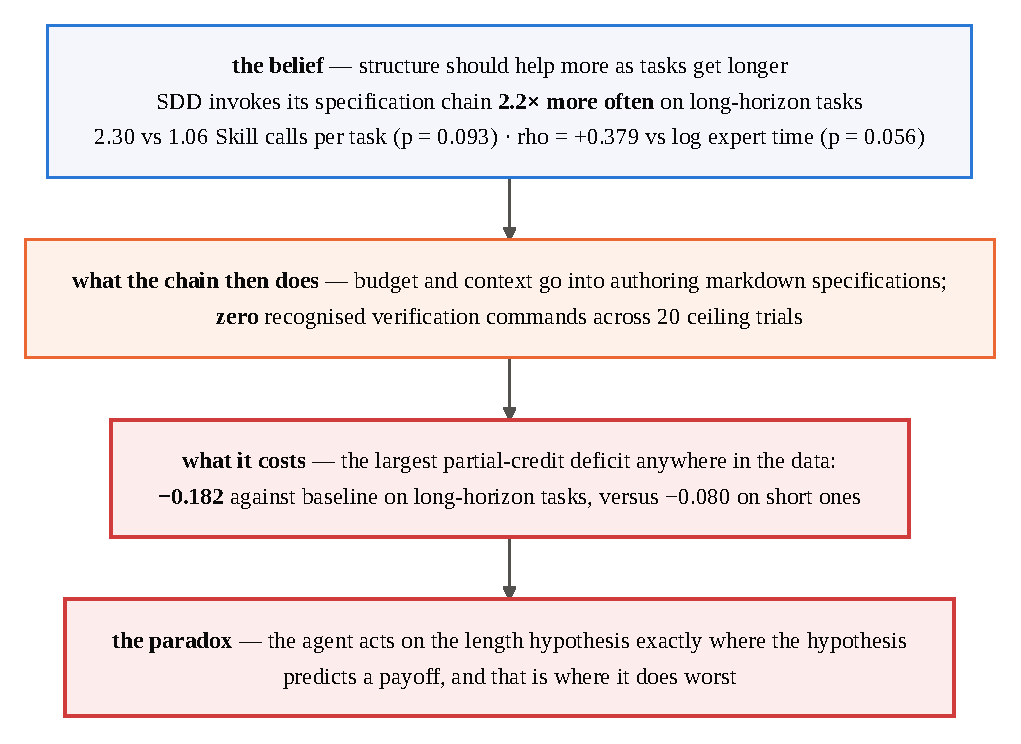
\includegraphics[width=0.86\linewidth]{diagrams/d05-methodology-paradox.pdf}
\caption{The paradox in full. The agent acts on the length hypothesis; the hypothesis does
not pay; and the largest deficit in the data sits exactly where the belief was strongest.}
\label{fig:paradox}
\end{figure}

That is a more pointed result than a null correlation. It is not ``we could not find the
effect where we looked''. It is ``the toolkit looked in the same place, acted on the same
belief, and the belief did not pay''.

\subsection{Why this analysis is confounded, and what would fix it}

\paragraph{The pooled sample mixes two populations selected on baseline outcome.} That is the
strongest confound available:

\begin{center}\small
\begin{tabular}{@{}lrr@{}}
\toprule
Baseline pass-at-2 & \emph{ceiling} run & \emph{suite} run \\
\midrule
short tasks & 1.000 ($n = 5$) & 0.455 ($n = 11$) \\
long-horizon tasks & 0.800 ($n = 5$) & 0.200 ($n = 5$) \\
\bottomrule
\end{tabular}
\end{center}

Run membership dominates baseline pass rate far more than long-horizon status does, so any
pooled regression on task properties partly measures \emph{which screen bucket a task fell
into}. Long-horizon tasks are split 5/5 between the runs, so the confound is not aligned with
the predictor --- but it is not orthogonal to it either. Within-run analysis would be clean
and is not possible: $n = 16$ and $n = 10$ give 80\,\% power only for $|\rho| \ge 0.65$ and
$\ge 0.79$.

\paragraph{Three further limits.}
\begin{itemize}
\item \textbf{The range is not the range the hypothesis is about.} These tasks top out at
      1{,}440 minutes of expert time in a \emph{single autonomous session} with a fully
      specified instruction. The hypothesis is about multi-session work with ambiguous
      requirements and a human in the loop. Nothing here reaches that regime.
\item \textbf{The budget wall censors the long end.} On the longest, tightest tasks the
      methodology conditions are frequently killed before finishing, so the outcome measure on
      exactly the tasks the hypothesis cares about most is the least reliable in the data.
\item \textbf{\code{expert\_min} is a poor predictor of anything about this agent}
      ($\rho = -0.078$ against baseline pass, $p = 0.704$). It measures human effort, not
      agent horizon.
\end{itemize}

\paragraph{What would actually test it}, in increasing order of cost:
\begin{enumerate}
\item Re-analyse with \code{steps\_to\_first\_passing\_test} as the length axis. It is already
      derived in both notebooks, it measures the agent's own horizon rather than a human's,
      and it costs nothing. Its limitation is that it only exists on tasks that produce a
      passing test.
\item Grade the workspace at kill time, so the long end stops being censored.
\item \textbf{Randomise invocation} --- mandate the methodology in half the trials --- so that
      ``enforcement'' becomes a manipulated variable rather than an observed one. This is what
      the hypothesis literally requires, and no run in this sequence has done it.
\item Build a task set stratified on agent horizon, with the two-sided screen of
      Section~\ref{sec:floor} and at least three attempts. At the rates observed here, roughly
      40 discriminating tasks $\times$ 3 conditions $\times$ 3 attempts $\approx$ 360 trials
      $\approx$ \$450--700.
\end{enumerate}

\clearpage
\section{Best-of-\emph{N} at equal spend: the strongest cross-run claim, adjudicated}
\label{sec:bestofn}

Repeated sampling is an established way to raise the functional correctness of model-written
code \citep{chen2021codex} and the accuracy of model reasoning \citep{wang2023selfconsistency},
and how to divide a fixed inference-time budget between one careful attempt and several cheap
ones is by now a research question in its own right \citep{snell2024scaling}. The claim below
is the software-process form of it.

The most consequential operational claim to come out of the independent review is this: given
a fixed budget, an engineering team should not equip its agent with a methodology; it should
run more independent attempts with the bare agent. The argument is arithmetic. If a single
CodeZen trial costs $k$ times a baseline trial, and the baseline's per-attempt pass rate is
$p$, then at equal spend baseline buys $k$ attempts and succeeds with probability

\[ P(\text{at least one of } k) = 1 - (1-p)^k. \]

On the \emph{suite} population, $k = 3.115$ per trial and $p = 0.25$, giving 59.2\,\% against
CodeZen's 36.0\,\% graded rate --- a gap of 23 percentage points at identical dollar spend.
Throughout this section $p$ is the per-attempt rate under reading 3 of
Section~\ref{sec:metrics}, all trials in the denominator with a censored trial keeping the
reward it scored, because that is the quantity a retry buyer actually purchases: the
probability that one paid attempt ends with a passing workspace. Under the punitive reading 2
the same arithmetic gives baseline $p = 0.219$, best-of-$k$ 53.7\,\% against CodeZen's
28.1\,\%, a gap of 26 points --- the conclusion is not sensitive to the choice.
The review's conclusion was that repeated independent sampling \emph{strictly dominates}
ceremonial methodology.

\subsection{The assumption that argument rests on}

The formula assumes every attempt on every task is an independent draw from one common
Bernoulli rate. That is two assumptions --- independence \emph{and} homogeneity --- and neither
follows from the sampling results above: those establish that \emph{more samples help}, not
that agent attempts on a fixed task are exchangeable. Independent evidence says they are not,
since between-run variance on agent benchmarks is substantial and structured rather than
uniform \citep{bjarnason2026randomness}. The two-attempt design gives a direct check on the
joint consequence.

\begin{figure}[htbp]
\centering
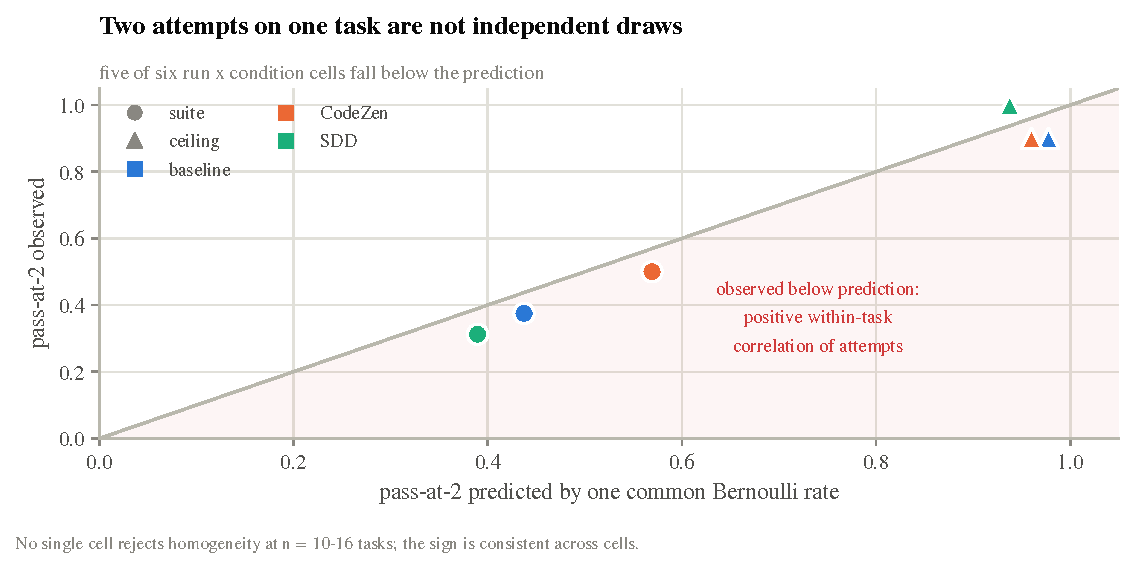
\includegraphics[width=0.80\linewidth]{figures/x14-attempt-independence.pdf}
\caption{Observed pass-at-2 against the value predicted by one common Bernoulli rate, for all
six run $\times$ condition cells. Five of six fall below the diagonal, which is the signature
of positive within-task correlation: tasks are not exchangeable, so a second attempt on a
task the agent already failed is worth less than a first attempt on a fresh one.}
\label{fig:independence}
\end{figure}

\begin{center}\small
\begin{tabular}{@{}llrrrr@{}}
\toprule
Run & Condition & $\bar p$ per attempt & pass-at-2 observed & predicted & counts 0/1/2 \\
\midrule
\emph{suite} & baseline & 0.250 & 0.375 & 0.438 & 10 / 4 / 2 \\
\emph{suite} & CodeZen & 0.344 & 0.500 & 0.569 & 8 / 5 / 3 \\
\emph{suite} & SDD & 0.219 & 0.313 & 0.390 & 11 / 3 / 2 \\
\emph{ceiling} & baseline & 0.850 & 0.900 & 0.978 & 1 / 1 / 8 \\
\emph{ceiling} & CodeZen & 0.800 & 0.900 & 0.960 & 1 / 2 / 7 \\
\emph{ceiling} & SDD & 0.750 & 1.000 & 0.938 & 0 / 5 / 5 \\
\bottomrule
\end{tabular}
\end{center}

\noindent No single cell rejects homogeneity --- the $\chi^2$ statistics on the 0/1/2 count
distributions range from 1.11 to 3.70 on 2 degrees of freedom, $p = 0.16$ to $0.57$, at
$n = 10$--$16$ tasks. But the \emph{sign} is consistent in five of six cells, and the
mechanism is not in doubt: in the \emph{suite} population, ten of sixteen tasks were failed
by baseline on both attempts. Retries cannot rescue a task that is dead.

\subsection{Three estimators, and the range they produce}

We therefore evaluate the equal-spend comparison under three models of baseline retry
success. In each, the condition keeps its actual two attempts and baseline receives $2k$
attempts for the same money.

\begin{description}[leftmargin=2.2em,style=nextline]
\item[Homogeneous] $1 - (1-\bar p)^{2k}$, with $\bar p$ the pooled per-attempt rate. Denies
      task heterogeneity entirely. This is the review's model, and it is the optimistic bound.
\item[Beta-binomial] Fit $\mathrm{Beta}(a,b)$ to the per-task success counts by maximum
      likelihood, then evaluate $1 - \mathbb{E}\left[(1-p)^{2k}\right]$. Smooths heterogeneity
      instead of denying or over-committing to it.
\item[Per-task plug-in] $\frac{1}{T}\sum_i \left[1 - (1-\hat p_i)^{2k}\right]$ with
      $\hat p_i$ estimated from that task's two attempts. Takes two-attempt estimates at face
      value, which over-commits on $\hat p_i = 0$ and is therefore the pessimistic bound.
\end{description}

\begin{table}[htbp]
\centering
\caption{Best-of-$N$ at equal spend, three estimators. The last column is CodeZen's actual
pass-at-2 rate on the same tasks for the same money.}
\label{tab:bestofn}
\small

\begin{tabular}{@{}lrrrrrr@{}}
\toprule
 & \multicolumn{1}{c}{baseline $\bar p$} & \multicolumn{1}{c}{$k$ at equal spend} &
 \multicolumn{3}{c}{baseline best-of-$k$, by estimator} & \multicolumn{1}{c}{CodeZen} \\
\cmidrule(lr){4-6}
run & per attempt & (2 CodeZen attempts) & homogeneous & beta-binomial & plug-in & pass-at-2 \\
\midrule
suite & 0.250 & 6.2 & 83.3\% & 58.6\% & 37.2\% & 50.0\% \\
ceiling & 0.850 & 3.4 & 99.9\% & 92.6\% & 89.1\% & 90.0\% \\
\bottomrule
\end{tabular}

\end{table}

\begin{figure}[htbp]
\centering
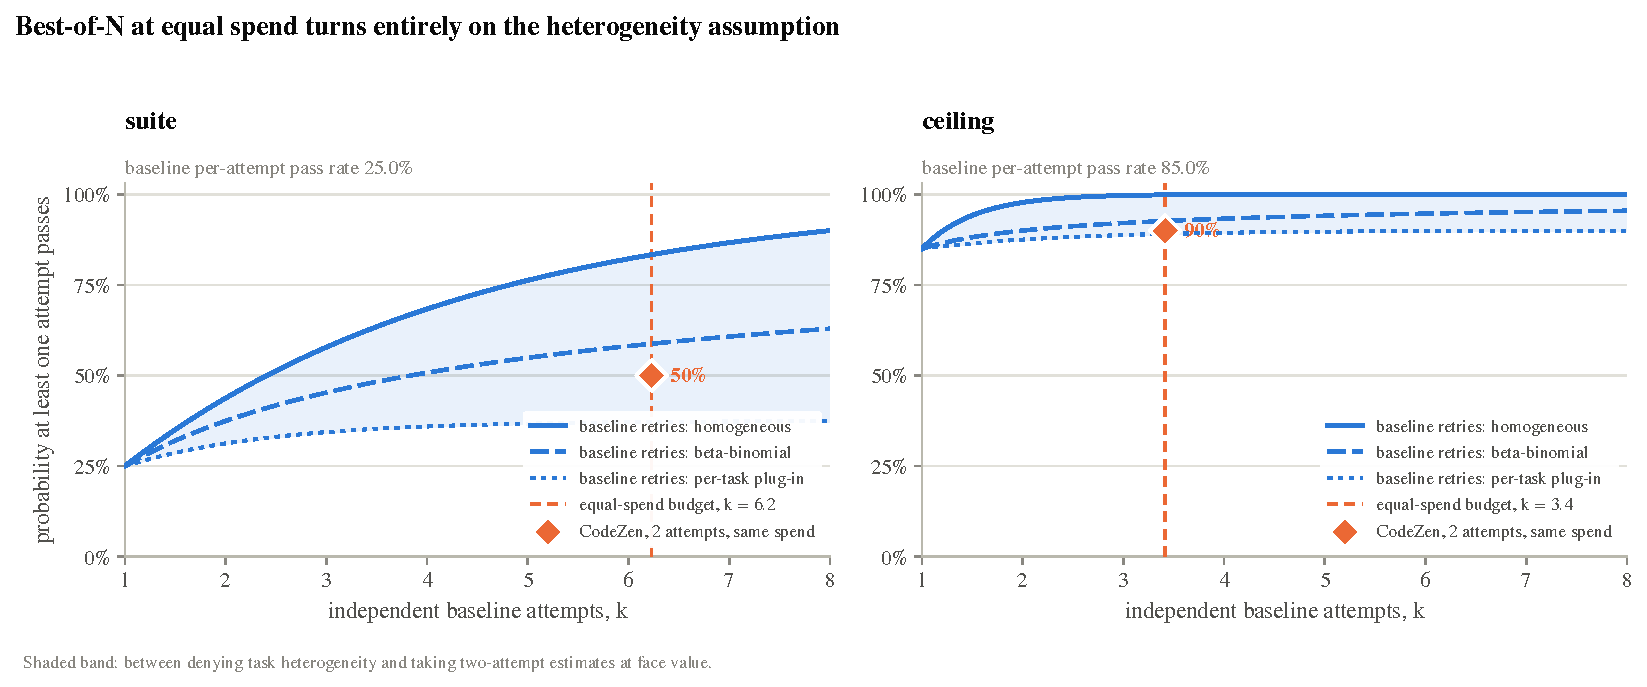
\includegraphics[width=\linewidth]{figures/x09-best-of-n.pdf}
\caption{Best-of-$N$ curves under the three estimators, with the equal-spend budget marked.
CodeZen's actual result sits \emph{inside} the band on the \emph{suite} population: above the
plug-in estimate, below the homogeneous one, and 8.6 points below the beta-binomial one.}
\label{fig:bestofn}
\end{figure}

\begin{finding}{The verdict: bounded, not settled}
On the \emph{suite} population, at 6.2 baseline attempts for the price of CodeZen's two, the
baseline retry strategy reaches somewhere between \textbf{37.2\,\% and 83.3\,\%} depending on
how task heterogeneity is modelled, against CodeZen's measured \textbf{50.0\,\%} pass-at-2.
The homogeneous model favours retries by 33 points; the beta-binomial model favours them by
8.6; the plug-in model favours \emph{CodeZen} by 12.8. The sign of the comparison changes with
the estimator, so the claim that repeated sampling strictly dominates methodology is
\textbf{not established by this data}. It remains the most plausible reading --- two of three
estimators favour retries, and the pessimistic estimator is the one with the clearest upward
bias in its assumptions --- but ``plausible'' is the correct word.
\end{finding}

\noindent On the \emph{ceiling} population the comparison resolves without needing an
estimator: baseline already passes 89.5\,\% of graded trials, so extra attempts buy almost
nothing, and the methodology's overhead is therefore a pure loss there rather than a trade.
All three estimators put baseline retries at or above CodeZen's 90.0\,\% for the same money.

\begin{finding}{What is still unmeasured, and is now the highest-value cheap experiment}
None of this is a measurement. Nothing in either run \emph{ran} baseline at 3$\times$ the
attempts and compared. That experiment costs no new infrastructure, is the comparison an
operator actually faces, and would replace a three-estimator range with a number.
\end{finding}

\clearpage
\section{Threats to validity and confounds}
\label{sec:threats}

These are carried forward unchanged from both source analyses, with two additions from the
recomputation.

\begin{description}[leftmargin=1.8em,style=nextline]

\item[The measured population is not the target population.] Terminal-Bench tasks are
single-session, self-contained and fully specified. Methodologies --- SDD explicitly --- are
written for multi-session work with ambiguous requirements and a human in the loop. This is
the regime in which a specification process has \emph{least} to add, and no result here
transfers to the regime in which it might have most. The requirements literature sharpens the
point in both directions: ambiguity in natural-language requirements is a longstanding and
consequential problem \citep{femmer2017smells}, and yet the effort spent hunting it is not
always repaid \citep{ribeiro2020ambiguity}. Evaluating a specification process therefore
requires task populations in which ambiguity and coordination are genuine sources of
difficulty --- a task-construction problem, not an analysis one. Nor is task-construction
defect hypothetical: a 2026 audit of a widely used coding benchmark reported a substantial
share of tasks affected by overly strict tests, underspecified prompts or insufficient
coverage \citep{openai2026signal}.

\item[The condition under test is a repository, not a methodology text.] Toolkits are
deployed in full, so \code{docs/}, \code{tools/}, \code{kits/} and \code{standards/} land in
the working directory alongside the task. What is measured is ``a repository configured this
way'', which is the ecologically valid unit but a broader one than ``the methodology''.

\item[\code{codezen-viable} is a curated four-skill subset] of an eleven-skill toolkit. Seven
CodeZen skills cannot run in a benchmark container. Every CodeZen number here is a number
about that subset, and nothing here speaks to \code{codezen-full}, which only ever ran on the
three-task probe.

\item[Method availability, not method enforcement.] The agent was never instructed to follow
the repository's process. With 71\,\% of toolkit trials invoking nothing
(Section~\ref{sec:adherence}), the experiment measures a configuration that is present and
mostly ignored. Whether that is a fact about the toolkits, the benchmark, or the agent, this
design cannot separate.

\item[Adherence instrumentation is textual.] It cannot see a \code{CLAUDE.md} the CLI loads
silently, and its shell-command buckets are pattern matches rather than parses. SDD's 0.00
verification commands is the most striking behavioural number in the paper and it rests on a
pattern match.

\item[Concurrency contention inflates the time metrics.] Nine trials ran at a time on one
host, so \code{agent\_sec}, \code{wall\_sec} and the derived \code{budget\_used} carry CPU and
I/O contention. Cost and token metrics are immune. Because contention is symmetric across
conditions within a task the paired comparisons survive; the absolute budget percentages do
not, and the budget wall is therefore partly a statement about how these runs were scheduled.

\item[The task partition may not be reliable enough to build a design on.] Every design in
this sequence assumes tasks sort into ``at ceiling'', ``discriminating'' and ``at floor''.
Section~\ref{sec:floor} shows that assignment failing in \emph{both} directions from a single
baseline trial. If the partition is unreliable, so is every conclusion that depends on which
bucket a task was put in.

\item[Effective sample size, stated plainly.] 18 of 26 tasks are concordant. The effective
$n$ per pairwise outcome comparison is 4--5 in \emph{suite} and 1--2 in \emph{ceiling}. No
outcome claim in this paper should be read as anything but underpowered.

\item[Two correlated tasks.] \task{path-tracing-reverse} (\emph{ceiling}) and
\task{path-tracing} (\emph{suite}) are siblings and are not independent samples in the pooled
analysis.

\item[Infrastructure faults, documented for completeness.] The \emph{suite} run lost a full
resume cycle to Docker address-pool exhaustion (25 orphaned compose networks from an
interrupted first pass exhausted the $\approx$31 default bridge subnets, and 54 trials died
before the agent started), and to root-owned bind-mount files blocking Harbor's cleanup.
Neither affected a recorded reward; both are fixed by configuration
(Section~\ref{sec:recommendations}).
\end{description}

\clearpage
\section{Independent review: where the two readings disagree}
\label{sec:divergence}

The primary analyses and the independent review by Antigravity (Google DeepMind) agree on
every qualitative conclusion in this paper. They disagree on nine quantities and on one
interpretation. Every disagreement was settled by recomputation from the exported per-trial
tables; the script is \code{whitepaper/scripts/}\allowbreak\code{verify\_numbers.py} and its output is
\code{whitepaper/data/}\allowbreak\code{verified\_numbers.json}.

\begin{table}[htbp]
\centering
\caption{Divergences between the two readings, and how each was settled. ``Recomputed'' is
the value this paper uses.}
\label{tab:divergence}
\footnotesize
\begin{tabular}{@{}p{3.5cm}p{3.3cm}p{3.3cm}p{4.6cm}@{}}
\toprule
Quantity & Primary reading & Independent review & Recomputed, and what follows \\
\midrule
\emph{ceiling} test-level pass rate &
90.7 / 92.6 / 68.5\,\% &
96.1 (49/51) / 96.4 (50/52) / 70.8 (37/52)\,\% &
\textbf{90.7 / 92.6 / 68.5\,\%} on 54 tests per condition. Passing counts 49/50/37 agree in
both; the review's denominators are wrong. Its derived claim --- a 22-point SDD deficit ---
survives either way (68.5 vs 90.7). \\
\addlinespace
\emph{ceiling} pass-both, baseline &
5 tasks pass in all three conditions (consistent with 8) &
``7 for baseline'' &
\textbf{8 of 10}. CodeZen 7, SDD 5. The review's ``5 of 10 vs 7'' understates baseline;
its conclusion that SDD's pass-both reliability collapses is unaffected. \\
\addlinespace
CodeZen \emph{ceiling} censored trials that had already passed &
3 of 6 (``half'') &
``4 of the 6'' in prose; its own itemised list shows 3 &
\textbf{3 of 6} scored reward 1.0; a fourth scored 0.67 partial. Internal inconsistency in
the review's prose, not a data disagreement. \\
\addlinespace
Toolkit skill calls, long vs short horizon &
2.30 vs 1.06 (SDD); 2.10 vs 1.50 (CodeZen) &
same &
Both are \emph{per-task totals across two attempts}. Per attempt the means are 1.15 vs 0.53
and 1.05 vs 0.75. The ratio ($2.17\times$) and $p$ (0.093) are identical either way. This
paper labels the unit explicitly. \\
\addlinespace
Best-of-$N$ at equal spend &
recorded as an open question, not computed &
57.8\,\% vs 36.0\,\%, ``strictly dominates'' &
Estimator-dependent: \textbf{37.2--83.3\,\%} against CodeZen's 50.0\,\%
(Section~\ref{sec:bestofn}). Two of three estimators favour retries; the sign changes with
the third. The claim is downgraded from ``strictly dominates'' to ``most plausible reading,
not established''. \\
\addlinespace
\task{headless-terminal} baseline
duration and cost &
not quoted &
253.4\,s and 648.9\,s, \$0.48 and \$0.78; ``exits immediately on green tests'' &
\textbf{144.5\,s and 114.1\,s, \$0.27 and \$0.20}, with \textbf{zero} recognised test
invocations on either attempt. The CodeZen/baseline ratio is $8.1\times$ and $14.1\times$, not
$3.6\times$ and $5.2\times$. CodeZen's own first-passing-test times, 65.6\,s and 58.5\,s, are
correct as stated. The trap is real and the contrast is larger than reported
(Section~\ref{sec:trap}). \\
\addlinespace
\task{torch-pipeline-}\newline\task{parallelism} baseline
reliability &
``baseline passes inside 34\,\% of budget'' &
``baseline succeeded easily inside 34\,\% of the budget''; also cites 1{,}175\,s &
Baseline passes \textbf{one of two} attempts at 29\,\% of budget; the other failed at 2 of 3
inside 38\,\%. 34\,\% is the mean of both. No baseline attempt took 1{,}175\,s (345.2 and
263.1\,s). The regression stands under pass-at-2; ``easily'' does not. \\
\addlinespace
SDD tasks dearer than baseline, \emph{ceiling} cost &
6 of 10 &
6 of 10 &
\textbf{7 of 10} by $\Delta > 0$. Ratio 1.097 and $p = 0.275$ are unaffected. \\
\addlinespace
CodeZen trials opening with
\code{noc-tdd} &
``nine of 12'' (\emph{suite}) &
not quoted &
\textbf{10 of 12} in \emph{suite}, and 5 of 7 in \emph{ceiling}. The pattern --- implement
first, review after --- is unchanged and slightly stronger. \\
\bottomrule
\end{tabular}
\end{table}

\subsection{Where the review's framing is retained in full}

Four contributions of the independent review are carried into this paper because they name
mechanisms the primary reading described but did not label:

\begin{enumerate}
\item \textbf{The post-completion timeout trap} (Section~\ref{sec:trap}). The primary reading
      recorded that four censored trials scored 1.0. The review reconstructed the
      \task{headless-terminal} trajectory and showed that the trial was solved in 66 seconds
      and then spent 834 seconds on ceremony. That is a mechanism, not a statistic, and it
      generates the sharpest architectural recommendation in the paper: an agent needs an
      explicit exit condition.
\item \textbf{The testing illusion} (Section~\ref{sec:behaviour}). $6.3\times$ the
      verification activity with \emph{lower} partial credit is explained by self-referential
      validation: an agent that writes its own tests encodes its own misreading of the
      specification and then confirms it.
\item \textbf{The screening fallacy as arithmetic} (Section~\ref{sec:floor}). Expressing the
      one-trial rule as a retention probability $1 - p_i$ turns a design criticism into a
      quantitative statement, and is what Figure~\ref{fig:screen} plots.
\item \textbf{The clock wall dominates the financial wall} (Section~\ref{sec:clock}).
      Agents under budget do not run out of money; they run out of time. Stated as an axiom it
      organises the whole of Section~\ref{sec:clock}.
\end{enumerate}

\subsection{Where this paper is more conservative than the review}

\begin{itemize}
\item The review presents its five conclusions as \textbf{axioms}. At $n = 26$ tasks with 18
      concordant, this paper presents them as findings with stated power, and separates
      ``settled'' from ``plausible'' from ``not resolved''.
\item The review's Axiom 5 (Best-of-$N$ dominance) is bounded rather than asserted
      (Section~\ref{sec:bestofn}).
\item The review reports ``CodeZen: 13 timeouts (25.0\,\% of all trials)''. The 13 and the
      25\,\% are correct, but the denominator is CodeZen's own 52 trials, not all 156. Stated
      as written it reads as a claim about the whole experiment.
\item The review's recommendation to select tasks with
      $\hat p_{\text{base}} \in [0.20, 0.75]$ is adopted, with the caveat that the
      discriminating band may be narrow and unstable --- in which case no screen produces a
      well-powered outcome comparison at affordable cost, and outcome should be demoted to a
      secondary endpoint. Both runs are consistent with that possibility; neither establishes
      it.
\end{itemize}

\clearpage
\section{What an operator should do with this}
\label{sec:operator}

\begin{figure}[htbp]
\centering
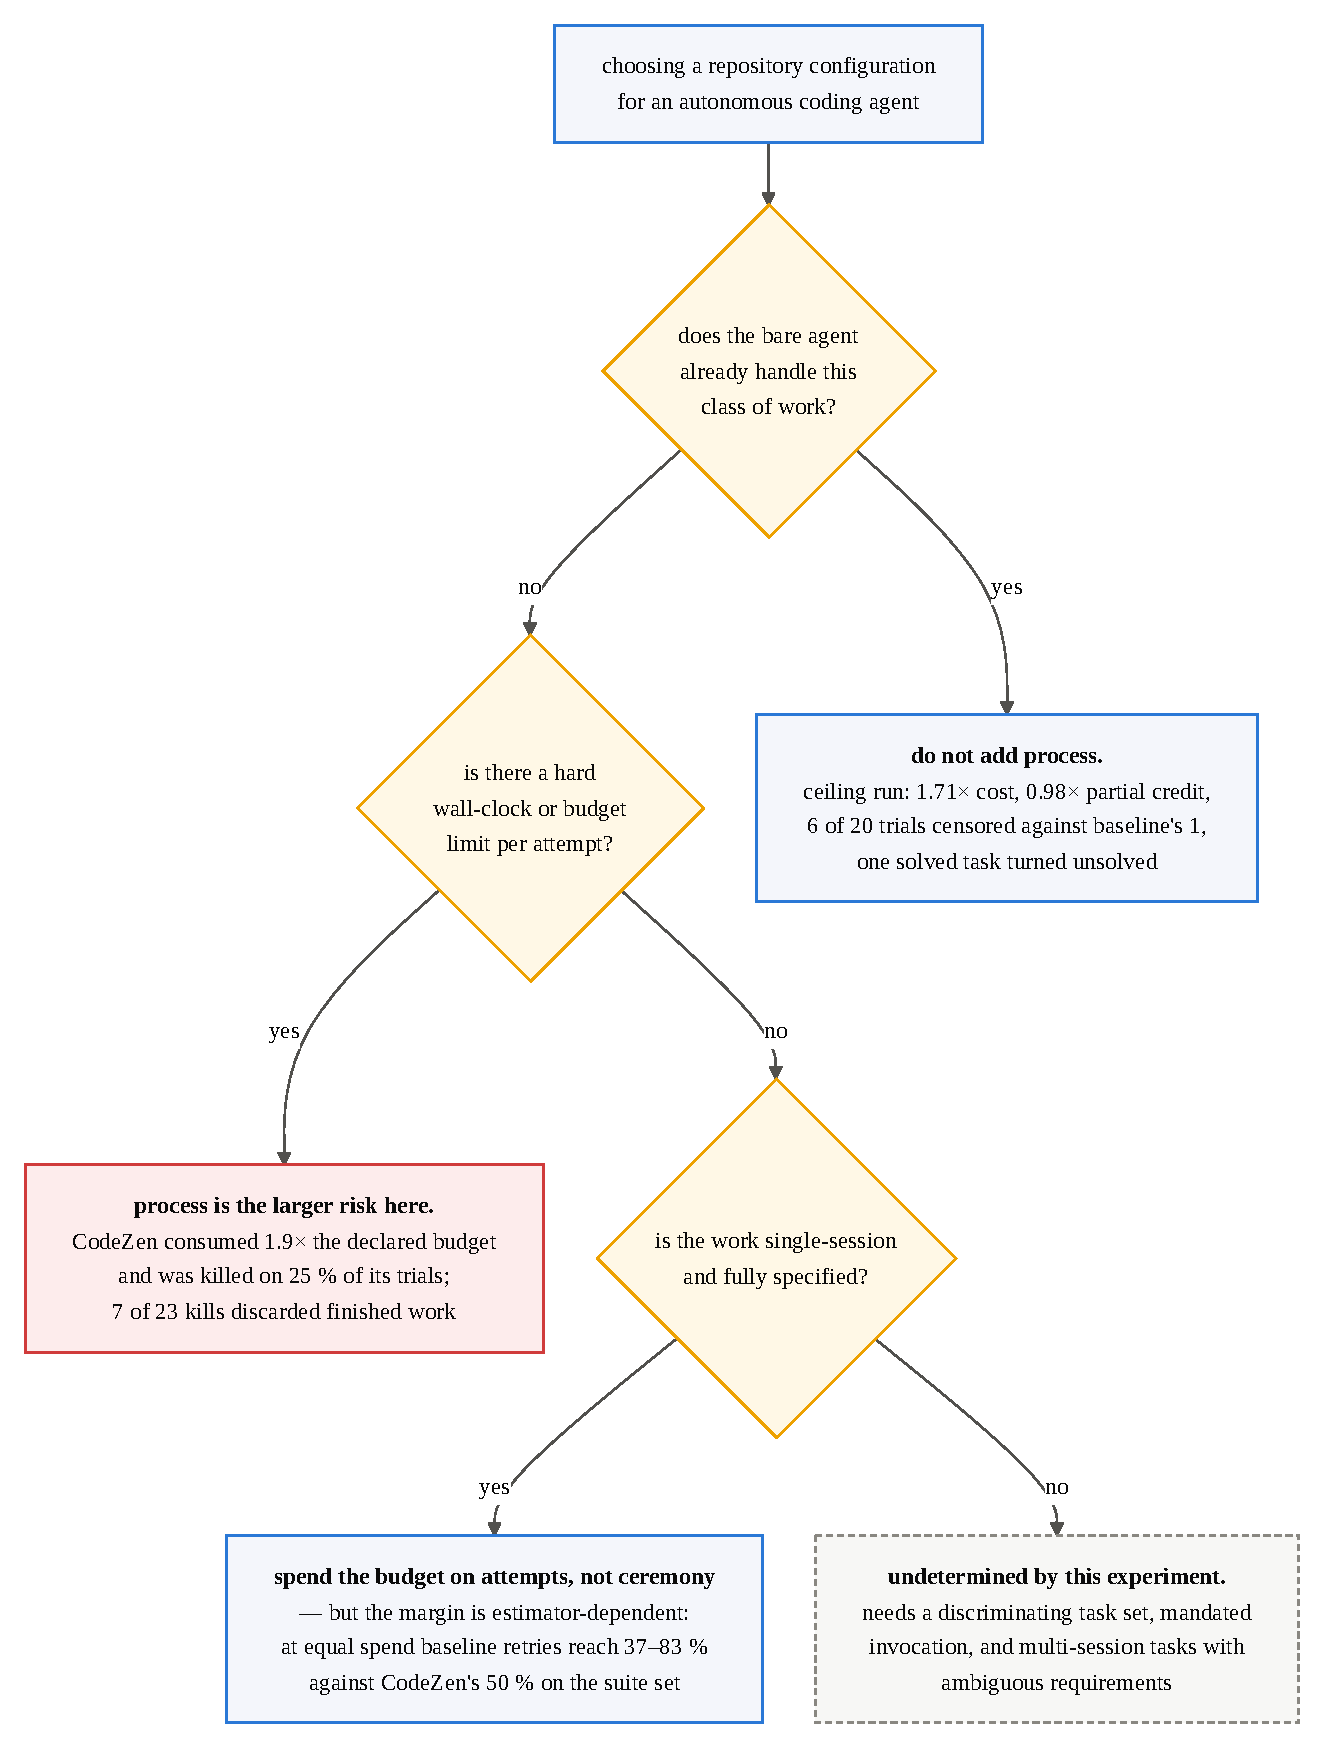
\includegraphics[width=0.88\linewidth]{diagrams/d07-operator-decision.pdf}
\caption{The decision the measurement actually supports, with the evidence attached to each
branch. Note that one branch is marked undetermined: this experiment does not reach the
regime methodologies are written for.}
\label{fig:decision}
\end{figure}

\begin{finding}{For a workload that resembles the \emph{ceiling} set --- code tasks the bare
agent handles}
The methodology is a $1.71\times$ cost with a measurable downside risk and no measurable
benefit. Baseline is 55\,\% cheaper per pass. At CodeZen's \$38.80, baseline would buy roughly
34 trials instead of 20 --- and since baseline already passes 89.5\,\% of them, those extra
attempts would be nearly wasted too. Neither more process nor more retries helps when the task
is already solved. The overhead is simply a loss.
\end{finding}

\begin{finding}{For a workload that resembles the \emph{suite} set --- tasks the bare agent
mostly fails}
Pay less and get the same. CodeZen bought two extra graded passes for \$46.26, inside the
noise band, at \$23.13 per marginal success against a baseline unit cost of \$3.12. Whether
the money is better spent on retries is the open question of Section~\ref{sec:bestofn}, and
the answer is estimator-dependent rather than obvious.
\end{finding}

\begin{finding}{Wherever there is a hard per-attempt time limit}
Process is the larger risk, not the cost. CodeZen consumed $1.90\times$ the declared budget
and was killed on 25\,\% of its trials; 7 of the 23 kills across both runs threw away
finished work. If a review or TDD skill can run after verification already passes, it will,
and it will sometimes cost the trial.
\end{finding}

\begin{finding}{The general form of the finding}
The result is not that these two toolkits are badly built. It is that a fixed process applied
unconditionally is the wrong shape of thing for an agent under a bounded budget.
Software-process research already holds that a standardised process should be tailored to its
project context \citep{xu2007tailoring}; the inference-time compute literature already holds
that the best use of an extra unit of compute depends on the difficulty of the instance
\citep{snell2024scaling}; and cost-aware agent evaluation already holds that resource
efficiency belongs among the dependent variables rather than outside them
\citep{liu2026costbench}. Read together, and against this experiment's evidence, they support
a single statement:

\smallskip
\emph{Autonomous coding methodology is better treated as an adaptive resource-allocation
policy than as a universally beneficial fixed process.}
\smallskip

This experiment supplies the concrete instance. The same review machinery that is defensible
while the artefact is still failing becomes harmful once it already passes, because continued
process consumes the one resource the trial needs in order to terminate --- and in seven
trials across both runs it converted finished work into a censored observation.
\end{finding}

\noindent Two engineering recommendations follow directly, and neither is about which
methodology to pick:

\begin{enumerate}
\item \textbf{State-aware skill gating.} An agent should check whether the verification
      criteria it can see are currently satisfied before initiating recursive review or
      refactoring sub-agents, and should refuse to start a delegated review with less than
      some fixed fraction of budget remaining.
\item \textbf{Sub-agent throttling on stalled workspaces.} If an agent has made zero
      successful file edits or test runs inside the first quarter of its budget, spawning
      skills are exactly what it should not reach for: that is the regime that produced the
      $3.11\times$ multiplier with no outcome to show for it.
\end{enumerate}

\clearpage
\section{Recommendations for the next run}
\label{sec:recommendations}

Ordered by value per dollar. The first four are the ones that change what the experiment can
conclude; the rest are hygiene.

\begin{table}[htbp]
\centering
\caption{Changes to make before another dollar is spent on this design.}
\label{tab:recommendations}
\small
\begin{tabular}{@{}p{6.6cm}p{9.2cm}@{}}
\toprule
Change & Why \\
\midrule
\textbf{Screen on baseline pass \emph{rate}, not a single baseline outcome.} Include a task
when baseline's pass rate over $\ge 3$ trials is strictly between 0 and 1, targeting
$\hat p_{\text{base}} \in [0.20, 0.75]$ &
The one-trial rule cannot distinguish ``always fails'' from ``sometimes fails'', and only the
second discriminates. Costs about 3 baseline trials per candidate instead of 1 --- roughly
$2\times$ the screen's original cost --- and it is the only change here that materially
improves the next run's power \\
\addlinespace
\textbf{Grade the working directory at the moment of the kill}, recording both
\code{timed\_out} and \code{functional\_score\_at\_kill} &
7 of 23 censored trials scored 1.0 anyway. Grading at kill time turns censoring from a lost
observation into a measured one, removes the need to choose a convention, and repairs the
long end of the length analysis. Costs no model tokens \\
\addlinespace
\textbf{Settle the censoring convention in writing, before the run} &
It moves CodeZen up to 27.9 points and changes its rank in the \emph{ceiling} run, from
first to second or third depending on the reading. Deciding after seeing the numbers is not a
defensible order of operations \\
\addlinespace
\textbf{Randomise methodology invocation}: mandate the process in half the trials &
Turns ``enforcement'' into a manipulated variable, breaks the selection/effect confound of
Section~\ref{sec:selection}, and answers the question most people actually mean when they ask
whether a methodology works \\
\addlinespace
\textbf{Run the equal-budget Best-of-$N$ comparison} &
One baseline trial at $2k$ attempts against one methodology trial, same tasks, same money.
Replaces the three-estimator range of Section~\ref{sec:bestofn} with a measurement \\
\addlinespace
Report pass-at-2 and pass-both side by side; name the aggregation in
\code{outcome\_matrix.csv} &
They disagree about whether SDD regressed 0 or 3 tasks, and the difference is exactly the
reliability question an operator cares about. The file currently writes pass-both under a name
implying pass-at-2 \\
\addlinespace
Parse verification commands instead of bucketing them by pattern &
SDD's 0.00 is the most striking behavioural number in the paper and it rests on a pattern
match \\
\addlinespace
Add a delegation column to \code{hmb report} &
2.55 sub-agents per CodeZen trial is its entire cost mechanism and the cell-level report
cannot see it \\
\addlinespace
Log a ``mock misalignment'' event when the agent's own test suite passes and the official
verifier fails &
This is the testing illusion of Section~\ref{sec:behaviour}, and it is currently invisible in
the data \\
\addlinespace
Re-verify the all-fail tasks and the two split \emph{ceiling} tasks against the oracle at
production concurrency &
Separates a genuine floor from a contention artefact, and settles whether
\task{make-mips-interpreter} and \task{torch-pipeline-parallelism} belong in either set.
Costs no model tokens \\
\addlinespace
Raise \code{--attempts} to 3 on a discriminating set &
Two attempts give a replicate but not a rate; three would let per-cell variance be reported,
and would sharpen the heterogeneity estimates of Section~\ref{sec:bestofn} \\
\addlinespace
Set \code{default-address-pools} in \code{/etc/docker/daemon.json}; add a \code{chown} repair
to \code{hmb resume} &
The two infrastructure faults of Section~\ref{sec:threats}. A \code{/16} base at
\code{size: 24} gives 256 networks instead of $\approx$31 \\
\addlinespace
Calibrate time budgets against agent active duration rather than raw container wall-clock when
running many trials concurrently &
Baseline wall-clock ran about 40\,\% above agent compute time at 9-way concurrency, and
\code{budget\_used} inherits that inflation \\
\bottomrule
\end{tabular}
\end{table}

\subsection{A blueprint for Methodology-Bench 2.0}

To move this from a decision-grade internal measurement to a publication-grade comparison,
four things must change together:

\begin{enumerate}
\item \textbf{Two-sided stratified screening.} About 30--40 tasks with baseline pass rates
      strictly inside $[0.20, 0.75]$ over at least 3 replicates, stratified on agent horizon
      rather than human-expert effort.
\item \textbf{Manipulated process.} Three regimes, not two: \emph{control} (bare baseline),
      \emph{autonomous} (methodology available in the repository, as measured here), and
      \emph{mandated} (the system prompt requires each step before solution code is written).
\item \textbf{Budget-equalised Best-of-$N$.} One methodology trial against $2k$ baseline
      attempts on the same tasks at the same spend.
\item \textbf{Interactive, under-specified environments.} Multi-turn tasks with incomplete
      specifications, where a specification-driven methodology has genuine ecological
      validity. Without this, the experiment keeps testing SDD in the one regime where it
      should be expected to add least.
\end{enumerate}

\noindent At the rates observed here, item 1 plus 3 attempts on 3 conditions is roughly 360
trials and \$450--700 of model spend. Items 2 and 4 are engineering, not spend.

\clearpage
\section{Open questions}
\label{sec:open}

These are questions about intent and design, not about data. Each changes how the same numbers
should be read.

\begin{enumerate}
\item \textbf{What decision does this measurement feed?} Choosing an internal default
      configuration, publishing a methodology comparison, and validating that a toolkit ships
      value are three different bars. The cost finding is decision-grade for the first and
      nowhere near publication-grade for the second.
\item \textbf{Which endpoint is primary --- outcome, cost, or conformance?} If the endpoint is
      cost at equal outcome, the question is settled for both populations, and the
      \emph{ceiling} run delivers it at $p = 0.002$ on a population where outcome is genuinely
      equal. If the endpoint is outcome, the design has to change before any answer exists. If
      it is conformance, both runs answer it identically: 71\,\% of toolkit trials invoked
      nothing.
\item \textbf{Should a timeout count as a failure?} Section~\ref{sec:outcome-ceiling} makes
      this concrete rather than theoretical, and grading at kill time is better than either
      convention.
\item \textbf{Is a regression on a ceiling task more or less serious than a failure on a hard
      one?} \task{torch-pipeline-parallelism} under CodeZen is a solved task made unsolved.
      Whether that outranks any amount of cost is a judgement about risk tolerance.
\item \textbf{Does the overhead beat $3\times$ the baseline attempts at equal budget?} The
      comparison an operator faces, cheap to run, and still untested
      (Section~\ref{sec:bestofn}).
\item \textbf{Is low adherence a toolkit property or a harness artefact?} Partially answered:
      SDD self-gates on task size ($\rho = +0.379$, $p = 0.056$), which is evidence for the
      first. CodeZen shows the same sign much more weakly.
\item \textbf{Should the methodology be mandated rather than merely available?} That is a
      different experiment answering a different question --- but it is the one most people
      mean when they ask whether a methodology works.
\item \textbf{Is a screened task set the right instrument at all?} Both screens overshot. If
      the discriminating band is narrow and unstable, the right response is to promote cost
      and conformance to primary endpoints and treat outcome as secondary.
\item \textbf{Which toolkit is the subject and which is the control?} If one of them is the
      artefact under development, the interesting design is a within-toolkit before/after
      against a fixed baseline, not a head-to-head --- and the power problem is far cheaper to
      solve in that framing.
\item \textbf{What would falsify the cost finding?} A population where the methodology's
      success rate exceeds baseline's by enough to justify $1.7\times$. Neither run has found
      one, and neither has looked where such a population would most plausibly live:
      multi-session work with ambiguous requirements and a human in the loop.
\end{enumerate}

\begin{finding}{Not worth more spend on the current design}
Another run on either of these task populations would reproduce the cost finding and add
nothing, because both populations are concordant for opposite reasons and the cost result is
already significant on both.
\end{finding}

\section{Reproducibility}
\label{sec:repro}

Everything in this paper is regenerable from the repository.

\begin{center}\small
\begin{tabular}{@{}ll@{}}
\toprule
Artefact & Path \\
\midrule
Per-trial tables (96 + 60 trials, 78 columns) & \code{results/analysis-\{suite,ceiling\}/data/trials.csv} \\
Per-test outcomes (357 + 162) & \code{.../data/tests.csv} \\
Per-step and per-tool-call telemetry & \code{.../data/\{steps,tool\_calls\}.csv} \\
Source analysis notebooks & \code{.../\{suite,ceiling\}\_analysis.ipynb} \\
Recomputation of every quoted number & \code{whitepaper/scripts/verify\_numbers.py} \\
Best-of-$N$ estimators and independence check & \code{whitepaper/scripts/best\_of\_n.py} \\
Figures (PDF + PNG) & \code{whitepaper/scripts/make\_figures\_\{perrun,cross\}.py} \\
Mermaid diagram sources and renderer & \code{whitepaper/diagrams/*.mmd}, \code{scripts/render\_diagrams.sh} \\
LaTeX tables & \code{whitepaper/scripts/make\_tables.py} \\
Verified values, as JSON & \code{whitepaper/data/verified\_numbers.json} \\
Pooled per-task table & \code{whitepaper/data/pooled\_task\_table.csv} \\
Literature review memo the citations follow & \code{whitepaper/data/schmierzettel.txt} \\
Bibliography, with \code{\% VERIFY} flags & \code{whitepaper/references.bib} \\
Citation placement and verification audit & \code{whitepaper/data/citation-map.md} \\
\bottomrule
\end{tabular}
\end{center}

\paragraph{Versions and pins.} Terminal-Bench 2.0 task suite at commit \code{2fd12b88};
agent Claude Code on \code{claude-sonnet-5}; both toolkits frozen at a Git SHA recorded in
\code{config/sources.yaml}. Runs executed 2026-08-31 (\emph{suite}) and 2026-09-01
(\emph{ceiling}) at 9-way concurrency on a single host.

\paragraph{Build.} \code{cd whitepaper \&\& make} regenerates figures, diagrams, tables and the
citation map, then compiles \code{main.pdf} and the short report \code{brief.pdf} with
Tectonic, which runs BibTeX itself. \code{make paper} and \code{make brief} compile only.

\section*{Acknowledgements}
\addcontentsline{toc}{section}{Acknowledgements}

The independent critical analysis of both runs and of the cross-run synthesis was contributed
by \textbf{Antigravity} (Google DeepMind). Its mechanistic reconstruction of the
post-completion timeout trap, its diagnosis of the screening rule as a retention probability,
and its framing of the clock as the binding constraint are carried into this paper
substantially as it stated them; Section~\ref{sec:divergence} records where the two readings
disagree and how each disagreement was settled.

\clearpage
\noindent\small\emph{Provenance of the reference list.} The literature set follows the review
memo in \code{data/schmierzettel.txt}. Entries whose bibliographic details could not be
confirmed first-hand --- chiefly the 2026 works --- are flagged by a \code{\% VERIFY} comment
above the entry in \code{references.bib}, and \code{data/citation-map.md} records every
placement together with three points where the memo's attribution appears to be wrong and what
was used instead. Verify those before circulating either document.\normalsize
\smallskip

\bibliographystyle{plainnat}
\bibliography{references}

\clearpage
\appendix
\section{Task tables}
\label{app:tasks}

\begin{table}[htbp]
\centering
\caption{The \emph{suite} population: 16 tasks the screen kept because one bare baseline trial
failed. ``ratio'' is expert estimate divided by declared agent budget. The last three columns
give attempts passed of two, per condition.}
\label{tab:tasks-suite}
\footnotesize
\resizebox{\linewidth}{!}{
\begin{tabular}{@{}lllrrrccc@{}}
\toprule
task & category & diff. & expert (min) & budget (min) & ratio & base & CZ & SDD \\
\midrule
\texttt{\footnotesize adaptive-rejection-sampler} & scientific-computing & medium & 180 & 15.0 & 12.0$\times$ & 0/2 & 1/2 & 1/2 \\
\texttt{\footnotesize cancel-async-tasks} & software-engineering & hard & 120 & 15.0 & 8.0$\times$ & 0/2 & 2/2 & 1/2 \\
\texttt{\footnotesize configure-git-webserver} & system-administration & hard & 15 & 15.0 & 1.0$\times$ & 1/2 & 0/2 & 0/2 \\
\texttt{\footnotesize extract-moves-from-video} & file-operations & hard & 120 & 30.0 & 4.0$\times$ & 0/2 & 0/2 & 0/2 \\
\texttt{\footnotesize filter-js-from-html} & security & medium & 45 & 30.0 & 1.5$\times$ & 0/2 & 0/2 & 0/2 \\
\texttt{\footnotesize git-multibranch} & system-administration & medium & 180 & 15.0 & 12.0$\times$ & 2/2 & 1/2 & 2/2 \\
\texttt{\footnotesize install-windows-3.11} & system-administration & hard & 300 & 60.0 & 5.0$\times$ & 0/2 & 0/2 & 0/2 \\
\texttt{\footnotesize openssl-selfsigned-cert} & security & medium & 20 & 15.0 & 1.3$\times$ & 1/2 & 2/2 & 2/2 \\
\texttt{\footnotesize path-tracing} & software-engineering & hard & 360 & 30.0 & 12.0$\times$ & 2/2 & 1/2 & 0/2 \\
\texttt{\footnotesize polyglot-c-py} & software-engineering & medium & 20 & 15.0 & 1.3$\times$ & 1/2 & 1/2 & 0/2 \\
\texttt{\footnotesize polyglot-rust-c} & software-engineering & hard & 180 & 15.0 & 12.0$\times$ & 1/2 & 2/2 & 1/2 \\
\texttt{\footnotesize raman-fitting} & scientific-computing & medium & 5 & 15.0 & 0.3$\times$ & 0/2 & 0/2 & 0/2 \\
\texttt{\footnotesize sam-cell-seg} & data-science & hard & 600 & 120.0 & 5.0$\times$ & 0/2 & 0/2 & 0/2 \\
\texttt{\footnotesize torch-tensor-parallelism} & software-engineering & hard & 240 & 15.0 & 16.0$\times$ & 0/2 & 1/2 & 0/2 \\
\texttt{\footnotesize train-fasttext} & model-training & hard & 30 & 60.0 & 0.5$\times$ & 0/2 & 0/2 & 0/2 \\
\texttt{\footnotesize video-processing} & video-processing & hard & 400 & 60.0 & 6.7$\times$ & 0/2 & 0/2 & 0/2 \\
\bottomrule
\end{tabular}
}
\end{table}

\begin{table}[htbp]
\centering
\caption{The \emph{ceiling} population: 10 of the 57 tasks the screen rejected as already
solved by the bare agent, ranked by expert/budget ratio. The two tasks that broke ranks ---
\task{make-mips-interpreter} and \task{torch-pipeline-parallelism} --- are the two highest
ratios in the set.}
\label{tab:tasks-ceiling}
\footnotesize
\resizebox{\linewidth}{!}{
\begin{tabular}{@{}lllrrrccc@{}}
\toprule
task & category & diff. & expert (min) & budget (min) & ratio & base & CZ & SDD \\
\midrule
\texttt{\footnotesize circuit-fibsqrt} & software-engineering & hard & 960 & 60.0 & 16.0$\times$ & 2/2 & 2/2 & 2/2 \\
\texttt{\footnotesize fix-ocaml-gc} & software-engineering & hard & 1440 & 60.0 & 24.0$\times$ & 2/2 & 2/2 & 2/2 \\
\texttt{\footnotesize headless-terminal} & software-engineering & medium & 120 & 15.0 & 8.0$\times$ & 2/2 & 2/2 & 1/2 \\
\texttt{\footnotesize make-mips-interpreter} & software-engineering & hard & 480 & 30.0 & 16.0$\times$ & 0/2 & 1/2 & 1/2 \\
\texttt{\footnotesize overfull-hbox} & debugging & easy & 60 & 12.5 & 4.8$\times$ & 2/2 & 2/2 & 2/2 \\
\texttt{\footnotesize path-tracing-reverse} & software-engineering & hard & 120 & 30.0 & 4.0$\times$ & 2/2 & 2/2 & 1/2 \\
\texttt{\footnotesize pypi-server} & software-engineering & medium & 60 & 15.0 & 4.0$\times$ & 2/2 & 2/2 & 2/2 \\
\texttt{\footnotesize schemelike-metacircular-eval} & software-engineering & medium & 300 & 40.0 & 7.5$\times$ & 2/2 & 1/2 & 1/2 \\
\texttt{\footnotesize sqlite-db-truncate} & debugging & medium & 60 & 15.0 & 4.0$\times$ & 2/2 & 2/2 & 2/2 \\
\texttt{\footnotesize torch-pipeline-parallelism} & software-engineering & hard & 240 & 15.0 & 16.0$\times$ & 1/2 & 0/2 & 1/2 \\
\bottomrule
\end{tabular}
}
\end{table}

\clearpage
\section{Every censored trial}
\label{app:censored}

\begin{table}[htbp]
\centering
\caption{All 23 trials killed by a Harbor timeout across both runs, with the reward the
verifier assigned to the workspace that was killed. Seven scored 1.0. Under the censoring
convention all 23 are dropped from both numerator and denominator; under
``timeout = failure'' all 23 count against their condition; under kill-time grading, seven of
them are successes.}
\label{tab:censored}
\small

\begin{tabular}{@{}lllrrrrr@{}}
\toprule
run & task & condition & reward & tests & partial credit & budget & cost \\
\midrule
suite & adaptive-rejection-sampler & CodeZen & 1.0 & 9/9 & 1.00 & 100\% & \$2.87 \\
suite & adaptive-rejection-sampler & CodeZen & 0.0 & 8/9 & 0.89 & 100\% & \$2.75 \\
suite & filter-js-from-html & CodeZen & 0.0 & 0/2 & 0.00 & 100\% & \$6.74 \\
suite & filter-js-from-html & CodeZen & 0.0 & 0/2 & 0.00 & 100\% & \$6.30 \\
suite & path-tracing & baseline & 1.0 & 5/5 & 1.00 & 100\% & \$3.22 \\
suite & path-tracing & SDD & 0.0 & 0/5 & 0.00 & 100\% & \$3.00 \\
suite & path-tracing & CodeZen & 0.0 & 0/5 & 0.00 & 100\% & \$2.73 \\
suite & path-tracing & SDD & 0.0 & 0/5 & 0.00 & 100\% & \$2.53 \\
suite & polyglot-rust-c & baseline & 0.0 & 0/1 & 0.00 & 100\% & \$0.65 \\
suite & polyglot-rust-c & SDD & 0.0 & 0/1 & 0.00 & 100\% & \$0.45 \\
suite & torch-tensor-parallelism & CodeZen & 1.0 & 3/3 & 1.00 & 100\% & \$2.62 \\
suite & train-fasttext & baseline & 0.0 & 0/2 & 0.00 & 100\% & \$0.39 \\
suite & train-fasttext & CodeZen & 0.0 & 1/2 & 0.50 & 100\% & \$1.22 \\
suite & train-fasttext & baseline & 0.0 & 0/2 & 0.00 & 100\% & \$0.70 \\
ceiling & headless-terminal & CodeZen & 1.0 & 7/7 & 1.00 & 100\% & \$2.21 \\
ceiling & headless-terminal & CodeZen & 1.0 & 7/7 & 1.00 & 100\% & \$2.79 \\
ceiling & make-mips-interpreter & CodeZen & 0.0 & 2/3 & 0.67 & 100\% & \$5.85 \\
ceiling & make-mips-interpreter & baseline & 0.0 & 0/3 & 0.00 & 100\% & \$4.94 \\
ceiling & make-mips-interpreter & SDD & 1.0 & 3/3 & 1.00 & 100\% & \$5.05 \\
ceiling & make-mips-interpreter & CodeZen & 1.0 & 3/3 & 1.00 & 100\% & \$4.42 \\
ceiling & path-tracing-reverse & SDD & 0.0 & 0/3 & 0.00 & 100\% & \$2.42 \\
ceiling & torch-pipeline-parallelism & CodeZen & 0.0 & 2/3 & 0.67 & 100\% & \$1.63 \\
ceiling & torch-pipeline-parallelism & CodeZen & 0.0 & 2/3 & 0.67 & 100\% & \$1.65 \\
\bottomrule
\end{tabular}

\end{table}

\clearpage
\section{Pooled correlations, in full}
\label{app:correlations}

\begin{table}[htbp]
\centering
\caption{Every Spearman rank correlation computed on the pooled 26-task table. At $n = 26$,
80\,\% power at $\alpha = 0.05$ two-sided requires $|\rho| \ge 0.53$, so every row below that
threshold means ``not resolved'', not ``absent''. Bold marks $p < 0.05$.}
\label{tab:correlations}
\small

\begin{tabular}{@{}lrrr@{}}
\toprule
Spearman rank correlation, pooled over 26 tasks & \multicolumn{1}{c}{$\rho$} & \multicolumn{1}{c}{$p$} & \multicolumn{1}{c}{$n$} \\
\midrule
baseline pass-at-2 vs log expert time & $-0.078$ & 0.704 & 26 \\
baseline absolute cost vs log expert time & $+0.696$ & \textbf{$<$0.001} & 26 \\
CodeZen cost \emph{ratio} vs log expert time & $+0.001$ & 0.996 & 26 \\
SDD cost \emph{ratio} vs log expert time & $+0.061$ & 0.767 & 26 \\
CodeZen cost ratio vs declared budget & $-0.005$ & 0.979 & 26 \\
CodeZen cost ratio vs instruction words & $+0.324$ & 0.106 & 26 \\
CodeZen absolute overhead vs log expert time & $+0.337$ & 0.093 & 26 \\
SDD absolute overhead vs log expert time & $+0.155$ & 0.448 & 26 \\
CodeZen timeouts vs expert/budget ratio & $+0.304$ & 0.131 & 26 \\
SDD timeouts vs expert/budget ratio & $+0.246$ & 0.225 & 26 \\
CodeZen skill calls vs log expert time & $+0.197$ & 0.335 & 26 \\
SDD skill calls vs log expert time & $+0.379$ & 0.056 & 26 \\
$\Delta$ pass-at-2, CodeZen, vs log expert time & $+0.222$ & 0.275 & 26 \\
$\Delta$ pass-at-2, SDD, vs log expert time & $+0.246$ & 0.225 & 26 \\
$\Delta$ pass-at-2, CodeZen, vs expert/budget & $+0.330$ & 0.099 & 26 \\
$\Delta$ pass-at-2, SDD, vs expert/budget & $+0.349$ & 0.081 & 26 \\
$\Delta$ pass rate, CodeZen, vs log expert time & $-0.028$ & 0.893 & 26 \\
$\Delta$ pass rate, SDD, vs log expert time & $+0.074$ & 0.720 & 26 \\
$\Delta$ pass rate, CodeZen, vs expert/budget & $+0.107$ & 0.602 & 26 \\
$\Delta$ pass rate, SDD, vs expert/budget & $+0.181$ & 0.376 & 26 \\
$\Delta$ partial credit, CodeZen, vs log expert time & $-0.028$ & 0.891 & 26 \\
$\Delta$ partial credit, SDD, vs log expert time & $-0.096$ & 0.642 & 26 \\
$\Delta$ partial credit, CodeZen, vs expert/budget & $-0.020$ & 0.923 & 26 \\
$\Delta$ partial credit, SDD, vs expert/budget & $+0.023$ & 0.910 & 26 \\
\bottomrule
\end{tabular}

\end{table}

\clearpage
\section{Pooled headline figures}
\label{app:pooled}

\begin{table}[htbp]
\centering
\caption{Pooled over both runs. The timeout row is the one to carry away: CodeZen's kill rate
is $2.6\times$ baseline's and SDD's.}
\label{tab:pooled}
\small

\begin{tabular}{@{}lrrr@{}}
\toprule
pooled over 156 trials, 26 tasks, \$201.37 & baseline & CodeZen & SDD \\
\midrule
cost per trial & \$0.858 & \$2.057 & \$0.958 \\
sub-agents spawned per trial & 0.038 & 2.596 & 0.019 \\
agent timeouts & 5 of 52 (9.6\%) & 13 of 52 (25.0\%) & 5 of 52 (9.6\%) \\
\bottomrule
\end{tabular}

\end{table}

\clearpage
\section{Figure and diagram index}
\label{app:index}

\begin{center}\footnotesize
\begin{tabular}{@{}llp{8.4cm}@{}}
\toprule
File & Kind & What it shows \\
\midrule
\code{suite-01-outcome} & figure & \emph{suite} outcome at three resolutions, Wilson intervals \\
\code{suite-02-outcome-matrix} & figure & \emph{suite} task $\times$ condition outcomes, attempts passed \\
\code{suite-03-overhead} & figure & \emph{suite} overhead indexed to baseline \\
\code{suite-04-budget} & figure & \emph{suite} budget consumption and censoring \\
\code{suite-05-behaviour} & figure & \emph{suite} behavioural profile \\
\code{suite-06-adherence} & figure & \emph{suite} availability versus adherence \\
\code{ceiling-01} \dots \code{-06} & figures & the same six views for the \emph{ceiling} run \\
\code{x07-cost-ratio-vs-length} & figure & cost multiplier against expert time, both runs \\
\code{x08-censoring} & figure & censoring split by verifier score at the kill \\
\code{x09-best-of-n} & figure & best-of-$N$ curves under three estimators \\
\code{x10-length-dissolution} & figure & length effect as metric resolution rises \\
\code{x11-adherence-vs-length} & figure & toolkit invocation against task horizon \\
\code{x12-cost-effectiveness} & figure & spend per pass and per passing test \\
\code{x13-screen-selection} & figure & what a one-trial screen selects for, analytically \\
\code{x14-attempt-independence} & figure & observed vs predicted pass-at-2 \\
\midrule
\code{d01-experiment-sequence} & diagram & the five-run sequence and each repair's overshoot \\
\code{d02-measurement-pipeline} & diagram & how a condition is built, proven and measured \\
\code{d03-post-completion-trap} & diagram & \task{headless-terminal} minute by minute \\
\code{d04-overhead-dynamics} & diagram & why one toolkit yields two cost multipliers \\
\code{d05-methodology-paradox} & diagram & SDD self-gates, then underperforms where it gated \\
\code{d06-screen-defect} & diagram & the one-trial screen's three misclassification modes \\
\code{d07-operator-decision} & diagram & the decision the measurement supports \\
\bottomrule
\end{tabular}
\end{center}

Diagram sources are Mermaid (\code{diagrams/*.mmd}) and are rendered to PDF and PNG by
\code{scripts/render\_diagrams.sh}; figures are generated by the two Matplotlib scripts in
\code{scripts/} directly from the exported CSV tables. Every artefact exists in both a vector
(PDF) and a raster (PNG) form.

\end{document}
